\documentclass{aa_stuff/aa} 

\usepackage{overhead}
\usepackage{newcommands}

%======================================================
%
%   Introduction stuff
%
%======================================================


\begin{document}
\title{Calculate the CMB power spectrum: \\
Cosmology II} 

\author{
Johan Mylius Kroken
\inst{1,2}
}
\institute{Institute of Theoretical Astrophysics (ITA), University of Oslo, Norway
\and
Center for Computing in Science Education (CCSE), University of Oslo, Norway}
%\email{nanna.bryne@fys.uio.no}}
\titlerunning{Calculating the CMB power spectrum}
\authorrunning{Mylius Kroken} 
\date{\today   \quad - \quad GitHub repository link: \url{https://github.com/Johanmkr/AST5220/tree/main/project}}  
\abstract{
    We consider linear perturbation to the FLRW cosmology in conformal Newtonian gauge in order to create a pipeline for predicting the power spectra of matter and anisotropies to the CMB. This is done by first calculating the background cosmology, and recombination epoch, including neutrinos. We then ignore neutrinos, polarisation and reionisation when evolving the perturbation equations in time, in order to solve for the power spectra which can be compared with observations. Ignoring these effects yielded a significant discrepancy in the result for small scale modes, but provide enough accuracy for the large scale modes. As a result, we obtained a pipeline through which we can obtain power spectra for different cosmologies and compare them to data, although the analysis is only done for the $\Lambda$CDM-cosmology using data from ~\cite{Planck2020}.
}

\maketitle
\bibliographystyle{aa_stuff/aa}

\tableofcontents

%======================================================
%
%   Section input
%
%======================================================



\newpage
\section*{Nomenclature}

\subsection*{Constants of nature}
\begin{itemize}
    \item[$m_e$] - Mass of electron.\\
        $m_e = 9.10938356\cdot10^{-31}\unit{kg}$.
    \item[$m_\mathrm{H}$] - Mass of hydrogen atom. \\
        $m_\mathrm{H} = 1.6735575\cdot10^{-27}\unit{kg}$.
    \item[$G$] - Gravitational constant.\\
            $G=6.67430$\stdf{-11}$\unit{m}^3\unit{kg}^{-1}\unit{s}^{-2}.$
    \item[$k_B$] - Boltzmann constant.\\
            $k_B = 1.38064852\cdot10^{-23}\unit{m}^2\unit{kg}\unit{s}^{-2}\unit{K}^{-1}.$
    \item[$\hbar$] - Reduced Planck constant.\\
            $\hbar = 1.054571817\cdot10^{-34}\unit{J}\unit{s}^{-1}$.
    \item[$c$] - Speed of light in vacuum.\\
            $c=2.99792458 \cdot10^8\unit{m}\unit{s}^{-1}$.
    \item[$\sigma_T$] - Thomson cross section.\\
            $\sigma_T = 6.6524587158\cdot10^{-29} \unit{m}^2$.
    \item[$\alpha$] - Fine structure constant.\\
        $\alpha = \frac{m_ec}{\hbar}\sqrt{\frac{3\sigma_T}{8\pi}}$
\end{itemize}

\subsection*{Cosmological parameters}
\begin{itemize}
    \item[$G_\munu$] - Einstein tensor.
    \item[$T_\munu$] - Stress-energy tensor.
    \item[$H$] - Hubble parameter.
%     \item[$H_0$] - Hubble constant \checkthis{fill in stuff}.
    \item[$\Hp$]  - Conformal Hubble parameter.
    \item[$T_{\mathrm{CMB}0}$] - Temperature of CMB today.
    \item[$a$] - Scale factor.
    \item[$x$] - Logarithm of scale factor.
    \item[$t$] - Cosmic time.
    \item[$z$] - Redshift.
    \item[$\eta$] - Conformal time.
    \item[$\chi$] - Co-moving distance. 
    \item[p] - Pressure.
    \item[$\rho$] - Density.
    \item[$r$] - Radial distance.
    \item[$d_A$] - Angular diameter distance.
    \item[$d_L$] - Luminosity distance.
    \item[] --------------------------
    \item[$n_e$] - Electron density.
    \item[$n_b$] - Baryon density. 
    \item[$X_e$] - Free electron fraction.
    \item[$\tau$] - Optical depth.
    \item[$\tilde{g}$] - Visibility function. 
    \item[$s$] - Sound horizon.
    \item[$r_s$] - Sound horizon at decoupling. 
    \item[$c_s$] - Wave propagation speed.
    \item[] --------------------------
    \item[$\Psi$] - Newtonian potential perturbation to the metric. 
    \item[$\Phi$] - Spatial curvature perturbation to the metric.
    \item[$P^\mu$]- Comoving momentum four vector.
    \item[$\mathcal{P}_l$] - Legendre polynomial of order $l$.
    \item[$k$] - Fourier mode $k=\vec{k}$ of wave vector $\vec{k}$. 
    \item[$\T$] - Photon perturbation.
    \item[$\T_l$] - $l$-th order multipole expansion term of $\T$.
    \item[$v_b$] - Baryon bulk velocity.
    \item[$v_c$] - Cold dark matter bulk velocity.
    \item[$v_\gamma$] - Photon bulk velocity. 
    \item[$\delta_b$] - Baryon overdensity.
    \item[$\delta_c$] - Cold dark matter overdensity.         
    \item[$\delta_\gamma$] - Photon overdensity.
    \item[$\phi$] - Inflaton field. 
    \item[$\rho_\phi$] - Inflaton field density.
    \item[$p_\phi$] - Inflaton field pressure.
    \item[$\epsilon_\mathrm{sr}, \delta_\mathrm{sr}$] - Slow roll parameters.  
    \item[$\mathcal{R}$] - Curvature perturbation.
    \item[$\mathcal{S}$] - Source function.  
    \item[] --------------------------
    \item[$\To$] - Observed temperature anisotropies.  
    \item[$Y_{lm}$] - Spherical harmonic functions.  
    \item[$a_{lm}$] - Coefficients in spherical harmonic expansion. 
    \item[$C_l$] - Angular power spectrum.
    \item[$P_\mathrm{prim}$] - Primordial power spectrum.
    \item[$n_s$] - Spectral index.
    \item[$A_s$] - Primordial amplitude.  
    \item[$\Delta_\mathrm{M}$] - Total matter contrast.
    \item[$P$] - Matter power spectrum. 
    \item[$j_l$] - Spherical Bessel function.  
\end{itemize}

\subsection*{Density parameters}
Density parameter $\O_X = \rho_X/\rho_\mathrm{crit}$ where $\rho_X$ is the density and $\rho_c=8\pi G/3H^2$ the critical density. $X$ can take the following values:
\begin{itemize}
    \item[$b$] - Baryons.
    \item[$c$] - Cold dark matter.
    \item[$\gamma$] - Electromagnetic radiation.
    \item[$\nu$] - Neutrinos.
    \item[$k$] - Spatial curvature.
    \item[$\Lambda$] - Cosmological constant.
\end{itemize}
A $0$ in the subscript indicates the present day value. 

\subsection*{Fiducial cosmology}
The fiducial cosmology used throughout this project is based on the observational data obtained by ~\cite{Planck2020}:
\begin{equation*}
        \begin{split}
                h &= 0.67, \\
                T_\mathrm{CMB0} &= 2.7255\unit{K}, \\
                N_\mathrm{eff} &= 3.046, \\
                \O_\mathrm{b0} &= 0.05, \\
                \O_\mathrm{c0} &= 0.267, \\
                \O_{k0} &= 0, \\
                \O_{\nu0} &= N_\mathrm{eff} \cdot \frac{7}{8}\left(\frac{4}{11}\right)^{4/3}\O_{\gamma0}, \\
                \O_{\Lambda0} &= 1- (\O_{k0} + \O_\mathrm{b0} + \O_\mathrm{CDM0} + \O_{\gamma0} + \O_{\nu0}),\\
                \O_\mathrm{M0} &= \O_{b0} + \O_\mathrm{CDM0}, \\
                \O_\mathrm{rad} &= \O_{\gamma0} + \O_{\nu0},\\
                n_s &= 0.965, \\
                A_s &= 2.1\cdot10^{-9}.
        \end{split}
\end{equation*}
\newpage
\section*{Introduction}\label{sec:introduction}

The Cosmic Microwave Background radiation is the leftover radiation from the early universe. It is the most ancient light we can observe, having travelled towards us ever since the Universe became transparent. Therefore, it contains a significant amount of information and it is of great interest to understand why it looks the way it does. Why are there fluctuations in the CMB? In this project we take a closer look at the CMB power spectrum. This is a plot that show the distribution of temperature fluctuations in the CMB across different angular scaler. This is of great significance to us, since the CMB power spectrum is able to reveal information about the cosmological parameters of our universe, such as the various density components and Hubble constant. It is also able to tell us something about the large scale structures of the Universe, and the overall geometry of space itself. Also, which is perhaps the most interesting, it can yield information about the nature of dark energy. 

The overarching aim is to produce a pipeline that allows us to calculate numerically the CMB power spectrum given some cosmology. The steps will be presented chronologically, and we start by setting up the background cosmology in ~\cref{sec:m1}. Here we solve the evolutionary equations for an isotropic and homogeneous universe using the $\Lambda$CDM-model. One particularly important event in the evolution of the CMB is recombination, ultimately leading to photon decoupling. After this, the photons free stream towards us and is what we today see as the CMB. The entire ~\cref{sec:m2} is devoted to this event, and the time right before and right after it. In ~\cref{sec:m3} we take a step away from the isotropic and homogeneous universe and consider perturbations to the metric in conformal Newtonian gauge. The implications these metric perturbations have on the distribution of matter is discussed, and we end up with a set of coupled differential equations that we can solve numerically. The initial condition of these are found by considering the period of inflation in the very early Universe. 

\TODO{Intro to Milestone 4}

\section{Background Cosmology}\label{sec:m1}

According to the cosmological principle, the universe is homogeneous and isotropic on a large scale. Hence, here are no preferred locations nor directions. Furthermore, we may safely assume that the physical laws that govern our local part of the universe is equally valid elsewhere, at larger distances. 

The aim now is to set up the background cosmology, in which the investigation of all interesting phenomena will take place. Setting up the background cosmology is practically equivalent to solving the \textit{Einstein field equation}:
\begin{equation}\label{eq:introduction:einstein_equation}
    G_\munu = 8\pi GT_\munu,
\end{equation}
where $G_\munu$ is the Einstein tensor describing the geometry of spacetime, $G$ is the gravitational constant and $T_\munu$ is the energy and momentum tensor. This equation thus relates the geometry and shape of spacetime itself, to its energy content (matter included). There are many solutions to ~\cref{eq:introduction:einstein_equation}, but we want the solution to govern a Universe that is spatially isotropic and homogeneous, but may evolve in time. The spacetime metric that satisfies this conditions is the \textit{Friedmann-Lemaître-Robertson-Walker metric} (FLRW)d ~\cite[ch. 8]{carroll_2019}.

We will use this metric in order to describe the background universe, how it may evolve in time, and its history. 

\subsection{Theory}\label{sec:m1:theory}

\subsubsection{Fundamentals}\label{sec:m1:theory:fundamentals}

    If we assume the universe to be homogeneous and isotropic, the line elements $\d s$ is given by the FLWR-metric, here in polar coordinates ~\cite[eq. 1.1.11]{weinberg2008cosmology}:
    \begin{equation}\label{eq:m1:theory:fundamentals:FLWR_line_element}
        \d s^2 = -\d t^2 + e^{2x}\left[ \frac{\d r^2}{1-kr^2}+r^2\d\theta^2 + r^2\sin^2\theta\d\phi^2 \right],
    \end{equation}
    where we have introduced $x = \ln(a)$ which will be our primary measure of time. 

    We further model all forms of energy in the universe as perfect fluids, only characterised by their rest frame density $\rho$ and isotropic pressure $p$, and an equation of state relating the two:
    \begin{equation}\label{eq:m1:theory:fundamentals:equation_of_state}
        \omega=\frac{\rho}{p}.
    \end{equation}
    By conservation of energy and momentum we must satisfy $\nabla_\mu T^\munu=0$, which results in the following differential equations for the density of each fluid $\rho_i$, from ~\cite{AST5220LectureNotes}:
    \begin{equation}\label{eq:m1:theory:fundamentals:density_diff_eq}
        \dv{\rho_i}{t} +3H\rho_i(1+\omega_i) = 0,
    \end{equation}
    where we have introduced the Hubble parameter $H \equiv\dot{a}/a=\d x/\d t$. The solution to ~\cref{eq:m1:theory:fundamentals:density_diff_eq} is of the form:
    \begin{equation}\label{eq:m1:theory:fundamentals:solution_to_density_diff_eq}
        \rho_i \propto e^{-3(1+\omega_i)x},
    \end{equation}
    where $\omega_\mathrm{M} = 0$ (matter), $\omega_\mathrm{rad}=1/3$ (radiation), $\omega_\Lambda=-1$ (cosmological constant) and $\omega_k=-1/3$ (curvature). 

    With these assumptions, the solution to the Einstein equations, \cref{eq:introduction:einstein_equation} are the Friedmann equations ~\cite[ch. 8.3]{carroll_2019}, the first of which describes the expansion rate of the universe:
    \begin{equation}
        \label{eq:m1:theory:fundamentals:first_friedmann_equation}
        H^2 = \frac{8\pi G}{3}\sum_i\rho_i - kc^2\expe{-2x} \\
    \end{equation}
    and the second describe how this expansion rate changes over time:
    \begin{equation}
        \label{eq:m1:theory:fundamentals:second_friedmann_equation}
        \dv{H}{t}+H^2 = -\frac{4\pi G}{3}\sum_i\left(\rho+\frac{3p}{c^2}\right).
    \end{equation}
    As of now, we are primarily interested in the first Friedmann equation. By introducing the critical density, $\rho_c\equiv2H^2/(8\pi G)$, we define the density parameters $\O_i=\rho_i/\rho_c$. We further define the density $\rho_k\equiv-3kc^2\expe{-2x}/(8\pi G)$,\footnote{This is the ``density of curvature'', but is in fact not a real density. It is called this because its mathematical behaviour is similar to that of the other (real) densities.} which enables us to write ~\cref{eq:m1:theory:fundamentals:first_friedmann_equation} as simply:
    \begin{equation}
        1=\sum_i\O_i,
    \end{equation}`
    where the density $\O_k$ is included in the sum. From ~\cref{eq:m1:theory:fundamentals:solution_to_density_diff_eq} we know the evolution of the densities in time, and if we assume the density values today, $\O_{i0}$, are known (or are free parameters), then ~\cref{eq:m1:theory:fundamentals:first_friedmann_equation} may also be written as:
    \begin{equation}\label{eq:m1:theory:fundamentals:Hubble_equation}
        H = H_0\sqrt{\sum_i\O_{i0}\expe{-3(1+\omega_i)x}},
    \end{equation}
    which is the Hubble equation we will use further.


\subsubsection{Measure of time and space}\label{sec:m1:measure_time_space}
    There are many ways of measuring time in cosmology, and they are often related to spatial quantities. The most common is perhaps the \textit{scale factor} $a$, which describes how the physical size of the universe changes with time. An increasing scale factor signifies an expanding universe and vice versa. Another, computationally more useful way of describing $a$ is through its logarithm $x=\ln a \iff a=e^x$, which is the convention we will stick to eventually.
    
    Another way of measuring the expansion of the Universe is through the \textit{redshift} $z$, which is defined as the change in wavelength of electromagnetic radiation between emitter and observer. Radiation propagates through the Universe, so any expansion (or contraction) would expand (or contract) the wavelength, and this is encapsulated in the redshift $z=\Delta\lambda/\lambda$. It is connected to the scale factor as $1+z=1/a$.
    
    Another, perhaps more familiar, time measure is the \textit{cosmic time} $t$. This is the time\footnote{In seconds, months, years, or any other preferred temporal unit (like the duration of a footbal match $\pm$ added time).} measured by a stationary observer (relative to the expanding universe). The statement: \textit{The Universe is somewhat 13 billion years old}, is given in cosmic time, i.e. the time we experience on Earth. 

    Lastly, there is the \textit{conformal time} $\eta$, defined as $\d\eta = c\d te^{-x}$.\footnote{The $c$ is sometimes omitted. $\d\eta = \d te^{-x}$ has units of $\unit{s}$, but multiplied with $c$ yields the distance traversed by a light ray in this time; which is the particle horizon.} This is a measure of distance (or rather the time it would take a light ray to traverse said distance) between points in space, where the expansion of space in between the points is taken into account. We use it to define the \textit{particle horizon}, which is the horizon generated by the maximal conformal time elapsed since the Big Bang. This is how ``far away'' from the Big Bang any light ray could have propagated (expansion of the Universe included). This horizon expands with time, as we would expect, and this is what we mean by conformal time from now on; the extent of the particle horizon, beyond which there cannot be any causal connection to the Big Bang. Thus, this is effectively the size of the causally connected universe. 

    Let's express this mathematically, starting with the cosmic time:
    \begin{equation}\label{eq:m1:theory:measures:cosmic_time}
        t = \int_0^a\frac{\d a}{aH} = \int_{-\infty}^{x}\frac{\d x}{H}.
    \end{equation}
    Using the definition of conformal time, we have:
    \begin{equation}\label{eq:m1:theory:measures:conformal_time}
        \eta = \int_0^a\frac{c\d a}{a^2H} = \int_{-\infty}^{x}\frac{c\d x}{e^xH} \equiv \int_{-\infty}^{x}\frac{c\d x}{\Hp},
    \end{equation}
    where $\Hp=e^xH$ is defined as the \textit{conformal Hubble parameter}. We may then define the \textit{comoving distance}, $\chi$, as the distance to a point, where we take the expansion of space into account, such that it becomes constant (given no relative motion). In contrast, the proper distance between two points increase as the universe increase, the comoving distance remain constant. It is related to the conformal time, and given by:
    \begin{equation}
        \label{eq:m1:theory:measures:conformal ditance}
        \chi = \int_1^a\frac{c\d a}{a^2H} = \int_0^x\frac{c\d x}{\Hp} = \eta_0-\eta,
    \end{equation}
    where $\eta_0$ is the conformal time today, and $\eta$ is the conformal time of the time we are measuring distance to.
    The radial coordinate in the FLRW line element, ~\cref{eq:m1:theory:fundamentals:FLWR_line_element}, is given in terms of the comoving distance and the curvature today $\O_{k0}$ as:
    \begin{equation}\label{eq:m1:theory:measures:r_equation_def}
        r = \begin{cases}
            \chi \cdot \frac{\sin\left(\sqrt{\abs{\O_{k0}}}H_0\chi/c\right)}{\sqrt{\abs{\O_{k0}}}H_0\chi/c} \qquad &\O_{k0} < 0 \\
            \chi \qquad &\O_{k0} = 0 \\
            \chi \cdot \frac{\sinh\left(\sqrt{\abs{\O_{k0}}}H_0\chi/c\right)}{\sqrt{\abs{\O_{k0}}}H_0\chi/c} \qquad &\O_{k0} > 0
        \end{cases}
    \end{equation}
    It is then straigtforward to define the angular diameter distance:
    \begin{equation}\label{eq:m1:theory:measures:angular_distance_def}
        d_A = \expe{x}r,
    \end{equation}
    and the luminosity distance:
    \begin{equation}\label{eq:m1:theory:measures:luminosity_distance}
        d_L = \expe{-x}r,
    \end{equation}
    both of which are derived in \cref{app:derivations}. The temporal quantities $\eta$ and $t$ have the following evolutions with $x$:
    \begin{equation}\label{eq:m1:theory:measures:eta_diffeq}
        \dv{\eta}{x} = \frac{c}{\Hp}.
    \end{equation}
    \begin{equation}\label{eq:m1:theory:measures:t_diffeq}
        \dv{t}{x} = \frac{1}{H}.
    \end{equation}
    Both differential equations are easy to solve numerically. Their derivation may also be found in \cref{app:derivations}

\subsubsection{$\Lambda$CDM-model}\label{sec:m1:lambdaCDM}

    In the $\Lambda$CDM model, the universe consists of matter in terms of baryonic matter ($b$) and cold dark matter (CDM), radiation in terms of photons ($\gamma$) and neutrinos ($\nu$) and dark energy in terms of a cosmological constant ($\Lambda$). In addition, we must allow for some curvature ($k$). As a result, the parameters of the model will be the present values of the Hubble rate, $H_0$, the baryon density $\O_{b0}$, the cold dark matter density $\O_{\mathrm{CDM}0}$, photon density $\O_{\gamma0}$, neutrino density $\O_{\nu0}$, dark energy density $\O_{\Lambda0}$, and the curvature density $\O_{k0}$. The present temperature of the cosmic microwave background radiation $T_{\mathrm{CMB}0}$ fixes the radiation density today through:
    \begin{equation}\label{eq:m1:theory:lambdaCDM:radiation_densities}
        \begin{split}
            \O_{\gamma0} &= \frac{16\pi^3G}{90}\cdot\frac{(k_b T_{\mathrm{CMB}0})^4}{\hbar^3c^5H_0^2}, \\
            \O_{\nu0} &= N_\mathrm{eff} \cdot\frac{7}{8} \cdot \left( \frac{4}{3} \right)^{4/3}\cdot \O_{\gamma0}.
        \end{split}
    \end{equation}
    The total radiation density is $\O_\mathrm{rad}=\O_\gamma+\O_\nu$ and the total matter density is $\O_\mathrm{M} = \O_b+\O_\mathrm{CDM}$.

    The Hubble equation from \cref{eq:m1:theory:fundamentals:Hubble_equation} may be redefined in terms of the conformal Hubble parameter $\Hp$ as:
    \begin{equation}\label{eq:m1:lambdaCDM:conformal_Hubble_equation}
        \begin{split}
            \Hp &= H_0\sqrt{U}\\
            U &\equiv \sum_i\O_{i0}\expe{-\alpha_ix}, 
        \end{split}
    \end{equation}
    where we have defined $\alpha_i\equiv(1+3\omega_i)$ and $i\in\{\mathrm{M}, \mathrm{rad}, \Lambda, k\}$. Since we know the values of the various $\omega_i$ it follows that:
    \begin{equation}
        \label{eq:m1:theory:lambdaCDM:alpha_values}
        \begin{split}
            \alpha_\mathrm{M} &= 1\\
            \alpha_\mathrm{rad} &= 2\\
            \alpha_k &= 0\\
            \alpha_\Lambda &= -2
        \end{split}
    \end{equation}

     Given the evolution of the density parameters with time, where the proportionality constant is the present day density, we introduce the \textit{radiation-matter equality}, i.e. the time radiation and matter densities were equal: $\rho_\mathrm{rad}=\rho_\mathrm{M}$. According to \cref{eq:m1:theory:fundamentals:solution_to_density_diff_eq} this can be expressed as:
     \begin{equation}\label{eq:m1:theory:equalities:radiation_matter}
        \begin{split}
            \rho_\mathrm{rad0}e^{-4x} &= \rho_\mathrm{M0}\expe{-3x} \\
            e^x &= \frac{\rho_\mathrm{rad0}}{\rho_\mathrm{M0}} \implies x_\mathrm{rM} = \ln\left(\frac{\O_\mathrm{rad0}}{\O_\mathrm{M0}}\right),
        \end{split}
     \end{equation}
     where $x_\mathrm{rM}$ now denotes the time of radiation-matter equality. 

     Similarly, the \textit{matter-dark energy equality}, where $\rho_\mathrm{M}=\rho_\Lambda$ can be found to be:
     \begin{equation}\label{eq:m1:theory:equalities:matter_dark_energy}
        \begin{split}
            \rho_\Lambda &= \rho_\mathrm{M0}\expe{-3x} \\
            \implies x_{\mathrm{M}\Lambda} &= \frac{1}{3}\ln\left(\frac{\O_\mathrm{M0}}{\O_\Lambda}\right)
        \end{split}
     \end{equation}
     Since $\Hp$ describes the expansion of the Universe, it is fair to say that the acceleration of the Universe is governed by its second derivative, and the acceleration onset may be found from the extremal point in its first derivative. This means that we find the acceleration onset when:
     \begin{equation}\label{eq:m1:theory:accel_onset_condition}
        \dv{\Hp}{x} = 0 \iff \dv{U}{x} = 0.
     \end{equation}
     This follows from ~\cref{eq:m1:lambdaCDM:conformal_Hubble_equation}. For further details on the derivative, see ~\cref{app:sanity}. We assume dark energy is involved in the acceleration of the universe, and thus assume the contribution from radiation is negligible. ~\cref{eq:m1:theory:accel_onset_condition} is thus further reduced to:
     \begin{equation}\label{eq:m1:theory:accel_onset_definiton}
        \begin{split}
            2\O_{\Lambda0}e^{2x} - \O_\mathrm{M0}e^{-x}&=0\\
            \implies x_\mathrm{accel}&=\frac{1}{3}\ln\left(\frac{\O_\mathrm{M0}}{2\O_{\Lambda0}}\right).
        \end{split}
     \end{equation}
    
    The age of the universe today, and the conformal time today can both be found by evaluating the solutions to the differential equations of $t$ and $\eta$ at the present time (where $x=0$). This is done numerically. 

\subsubsection{Analytical solutions and sanity checks}\label{sec:m1:theory:sanity}
    There are several ways we may check that both our workings and numerical implementations are indeed correct. The simplest way is to always ensure that the sum of all density parameters add up to 1, for all times: $\sum_i\O_i=1$. 
    
    If we only consider the most dominant density parameter, that is $\O_i \gg \sum_{j\neq i}\O_j$, we end up with the following analytical expressions for different temporal regimes:
    \begin{equation}
        \label{eq:m1:theory:sanity:first_deriv_sanity}
        \frac{1}{\Hp}\dv{\Hp}{x} \approx - \frac{\alpha_i}{2} = 
        \begin{cases}
            -1 \qquad &\alpha_\mathrm{rad} = 2 \\
            -\frac{1}{2} \qquad &\alpha_\mathrm{M} = 1\\
            1 \qquad &\alpha_\Lambda = -2
        \end{cases}
    \end{equation}
    \begin{equation}
        \label{eq:m1:theory:sanity:second_deriv_sanity}
        \frac{1}{\Hp}\dv[2]{\Hp}{x} \approx \frac{\alpha_i^2}{4} = 
        \begin{cases}
            1 \qquad &\alpha_\mathrm{rad} = 2 \\
            \frac{1}{4} \qquad &\alpha_\mathrm{M} = 1\\
            1 \qquad &\alpha_\Lambda = -2
        \end{cases}
    \end{equation}
    \begin{equation}
        \label{eq:m1:theory:sanity:conformal_hubble}
        \Hp \approx H_0\sqrt{\O_{i0}e^{-\alpha_ix}} = 
        \begin{cases}
            H_0\sqrt{\O_\mathrm{rad0}}e^{-x} \qquad &\alpha_\mathrm{rad} = 2 \\
            H_0\sqrt{\O_\mathrm{M0}}e^{-x/2} \qquad &\alpha_\mathrm{M} = 1\\
            H_0\sqrt{\O_{\Lambda0}}e^x \qquad &\alpha_\Lambda = -2
        \end{cases}
    \end{equation}
    \begin{equation}
        \label{eq:m1:theory:sanity:eta_sanity}
        \frac{\eta\Hp}{c} \approx 
        \begin{cases}
            1 \qquad &\alpha_\mathrm{rad} = 2 \\
            2 \qquad &\alpha_\mathrm{M} = 1\\
            \infty \qquad &\alpha_\Lambda = -2
        \end{cases}
    \end{equation}
    These equations will be useful when making sure that the implementations are correct.\footnote{~\cref{eq:m1:theory:sanity:eta_sanity} is a bit hand-wavy as $\eta$ is really an integral, so assuming a dominant density parameter, means assuming it for the whole existence of the universe, not only the regime we are looking at. We may hence expect these to bee gradually more wrong as the Universe evolves. \TODO{DO I HAVE TIME TO FIX THIS?}} For a thorough derivation, see \cref{app:sanity}.




\subsection{Methods}\label{sec:m1:methods}

\subsubsection{Initial equation}
    We have to consider the time evolution of the density parameters, given some present value, as function of our chosen time parameter, here $x$. The density evolution is implemented as:
    \begin{equation}\label{eq:m1:methods:initial:density_evolution}
        \O_n = \expe{-\alpha_nx}\O_{n0}\Hp_\mathrm{rat}^2
    \end{equation}
    where we have defined the ratio $\Hp_\mathrm{rat} \equiv H_0/\Hp$, and the new index $n$ are all the densitis: $n\in\{b, \mathrm{CDM}, \gamma, \nu, \Lambda, k\}$.

    We also implement functions to solve for the luminosity distance (\cref{eq:m1:theory:measures:luminosity_distance}), angular distance (\cref{eq:m1:theory:measures:angular_distance_def}), and the conformal distance (\cref{eq:m1:theory:measures:conformal ditance}).


\subsubsection{ODEs and Splines}
    The differential equations for $\eta$ (\cref{eq:m1:theory:measures:eta_diffeq}) and $t$ (\cref{eq:m1:theory:measures:t_diffeq}) are solved numerically as ordinary differential equations with the Runge-Kutta 4 as advancement method. The equations are solved for $x\in(-20,5)$. As initial condition we would like $\eta(-\infty)$ which is obviously not possible to calculate, so we pick some very early time and use the analytical approximation in the radiation dominated era (\cref{eq:m1:theory:sanity:eta_sanity}), which yield:
    \begin{equation}\label{eq:m1:methods:odes:eta_initial}
        \eta(x_0) = \frac{c}{\Hp(x_0)}.
    \end{equation}
    Likewise for $t$, the initial condition is:
    \begin{equation}\label{eq:m1:methods:odes:t_initial}
        t(x_0) = \frac{1}{2H(x_0)}.
    \end{equation}
    \FIXME{WHY divided by 2?}
    
    We then proceed by making splines of both $\eta$ and $t$. 

    
\subsection{Results and discussion}\label{sec:m1:results}

\subsubsection{Tests}\label{sec:m1:results:tests}
    ~\cref{fig:m1:omega_tests} show the evolution of the density fractions with time. They sum to one across all times which was required. At early times the radiation density dominates (orange line). The intersection between the orange and green lines mark the radiation-matter equality, after which matter is the dominating density. Likewise, the intersection between the green and purple lines mark the matter-dark energy equality, where dark energy (manifested in the cosmological constant) become the dominating density. Time can thus be divided into three regimes; radiation dominated, matter dominated, and dark energy dominated eras, separated by black dotted lines in the plot. 
    \begin{figure}
        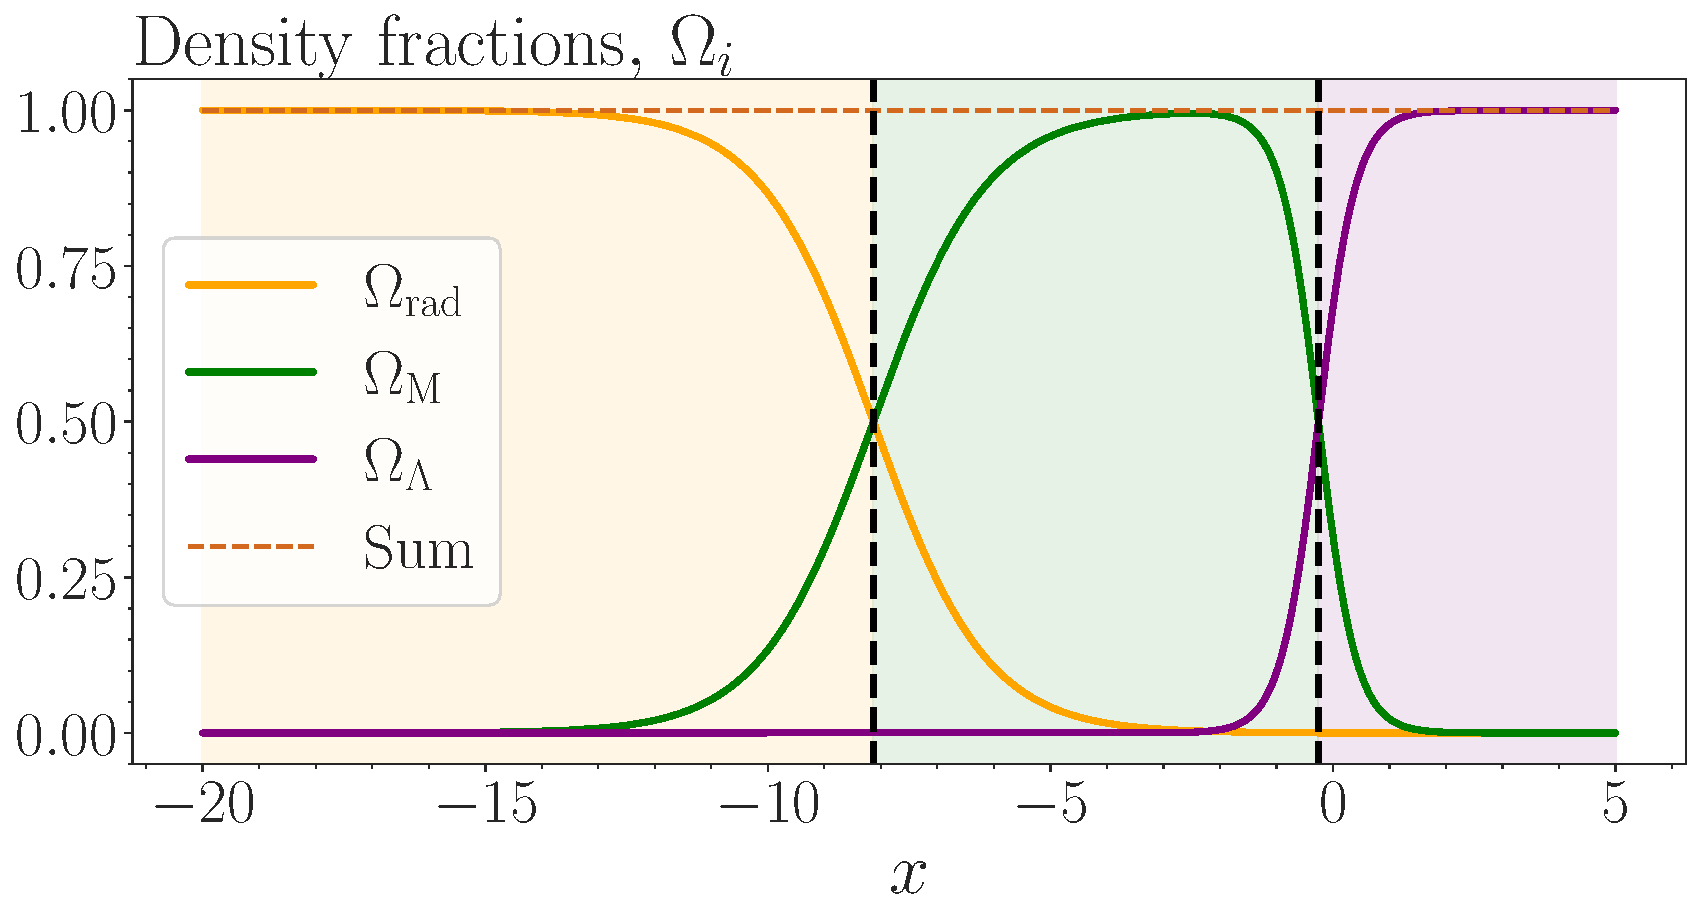
\includegraphics[width=\linewidth]{testing_omegas.pdf}
        \caption{Density fractions $\O_i$ as function of $x$. For low $x$, radiation dominates, before matter dominates and dark energy has just become the dominant energy density today $x=0$, and will continue to dominate into the future. The sum of densities sums to one across all times, as required (white dotted line). The black dotted lines are the radiation-matter equality at $x=-8.13$ and the matter-dark energy equality at $x=-0.26$, both stated in ~\cref{tab:m1:important_values}. The domination of each regime is shown as a shaded background with similar colour as its respective graph. }
        \label{fig:m1:omega_tests}
    \end{figure}
    
    \TODO{fix this}
    As explained in section ~\cref{sec:m1:theory:sanity}, we have analytical solutions for constructions of $\eta$ and $\Hp$ in the different regimes. \cref{fig:m1:eta_tests} is the sanity check for $\eta$, showing $\eta\Hp/c$ converging to finite values in the radiation and matter dominated eras (where $\alpha_{\mathrm{rad}, \mathrm{M}}>0$), and diverging towards $+\infty$ in the dark energy dominated era ($\alpha_\Lambda =-2 <0$). This is in accordance with the analytical solutions. The different regimes are shown in shaded colour. It is also worth noticing that $(\d \eta /\d x)\Hp/c$ is one for all regimes, as expected from equation ~\cref{eq:m1:theory:measures:eta_diffeq}. \TODO{to this}

    \begin{figure}
        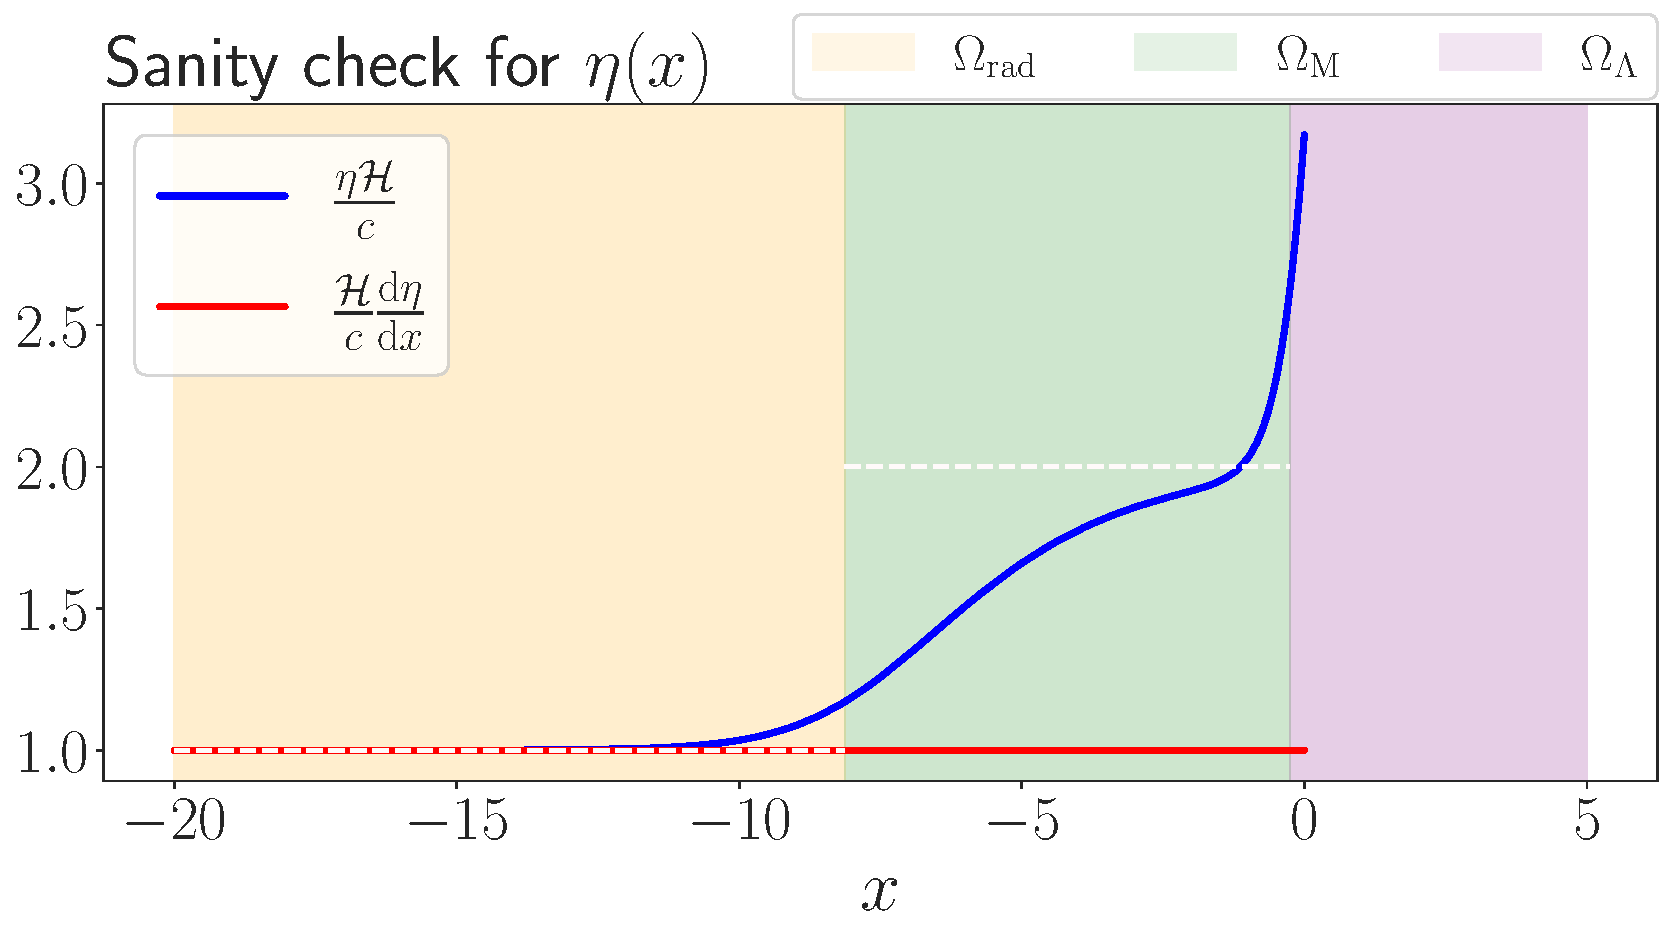
\includegraphics[width=\linewidth]{eta_test.pdf}
        \caption{Sanity check for $\eta$. $\eta\Hp/c$, in blue, is 1 in the radiation regime, 2 in the matter regime and diverging toward $+\infty$ in the dark energy regime, as expected from the analytical approximations in each regime. Remembering that this is strictly correct only in the radiation regime explains the mismatch of the brown doted line in the matter regime. $(\d \eta /\d x)\Hp/c$, in red, is 1 throughout time, as expected from ~\cref{eq:m1:theory:measures:eta_diffeq}.}
        \label{fig:m1:eta_tests}
    \end{figure}

    ~\cref{fig:m1:Hp_tests} is the sanity check confirming that our constructions of $\Hp$ and its derivatives converge to the analytical approximation in the different regimes. The second derivative, as shown in blue, takes the value of 1 in the radiation regime, 1/4 in the matter regime and 1 in the dark energy regime. Similarly, the first derivative, as shown in red, take the value -1 in the radiation regime, -1/2 in the matter regime and 1 in the dark energy regime. This is well in accordance with the analytical approximations put forth in section ~\cref{sec:m1:theory:sanity}. 

    \begin{figure}
        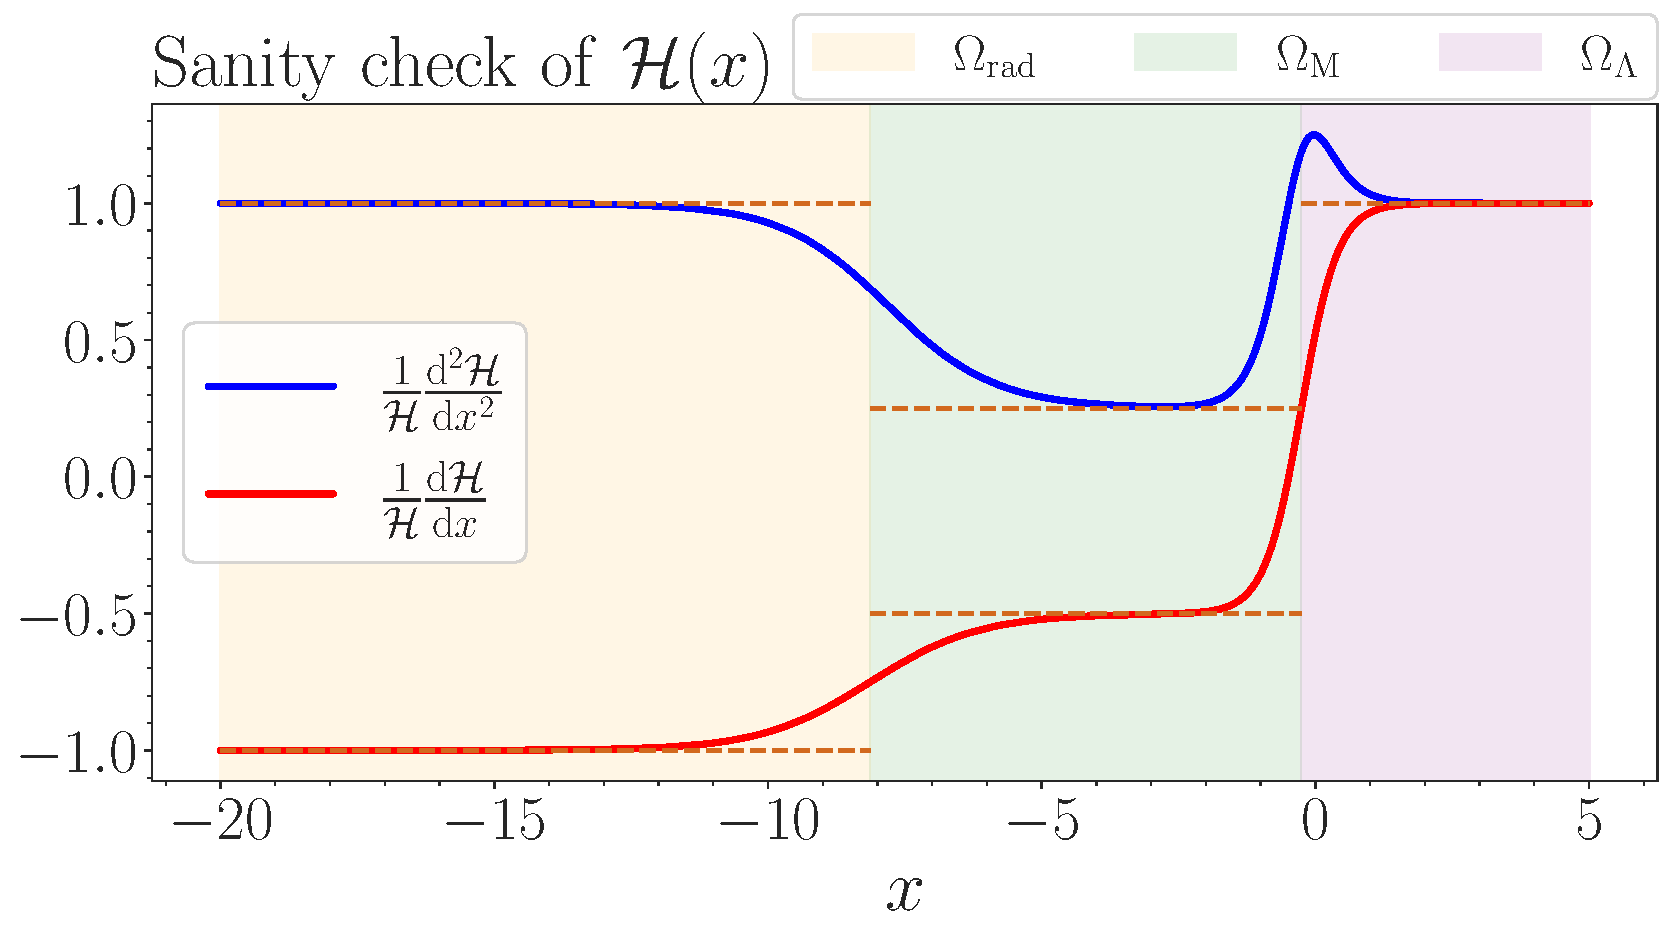
\includegraphics[width=\linewidth]{Hp_test.pdf}
        \caption{Sanity check for $\Hp$, showing that the second derivative (blue) converge to the analytical expressions shown as brown dotted lines in the different regimes. The first derivative (red) converge to its analytical values in the same regimes, which again are shown with a shaded colour.}
        \label{fig:m1:Hp_tests}
    \end{figure}

    These sanity checks are confirmations that the implementations yield the same result as the analytical approximation in the different regimes for various constructions of $\eta$ and $\Hp$ and their derivatives.
    
\subsubsection{Analysis}

    In ~\cref{sec:m1:lambdaCDM} we indicate how we can calculate the radiation-matter equality (RM-equality), matter-dark energy equality (ML-equality), when the acceleration of the universe started, the age of the universe and the conformal time today. The result is shown in ~\cref{tab:m1:important_values}. We note that the equalities is in accordance with the sanity checks, and the age of the universe today (in cosmic time) is about 13.9 Gyr. We also note that the acceleration onset is slightly before the matter-dark energy equality at $x=-0.49$ and $x=-0.26$ respectively. 
    \begin{table}
        \begin{tabular}{lrrrl}
Quantity & x & z & t [Gyr] &  \\
RM-equality  & -8.13 & 3400.33 & 0.000051 &   \\
ML-equality  & -0.26 & 0.29 & 10.378200 &   \\
Accel. start  & -0.26 & 0.29 & 10.378200 &    \\
Age of universe  & 0.00 & 0.00 & 13.857700 &   \\
Conformal time  & 0.00 & 0.00 & 46.318700 &   \\
\end{tabular}

        \caption{Important quantities in the evolution of the universe. RM stands for radiation-matter and ML for matter-dark energy.}
        \label{tab:m1:important_values}
    \end{table}

    The conformal Hubble factor, $\Hp$, is plotted against time, $x$, in ~\cref{fig:m1:conformal_hubble_factor_Hp}. It is decreasing in the radiation and matter regimes and increasing in the dark energy regime, switching signs at the acceleration onset, which is marked with a black dotted line in the figure. 
    \begin{figure}
        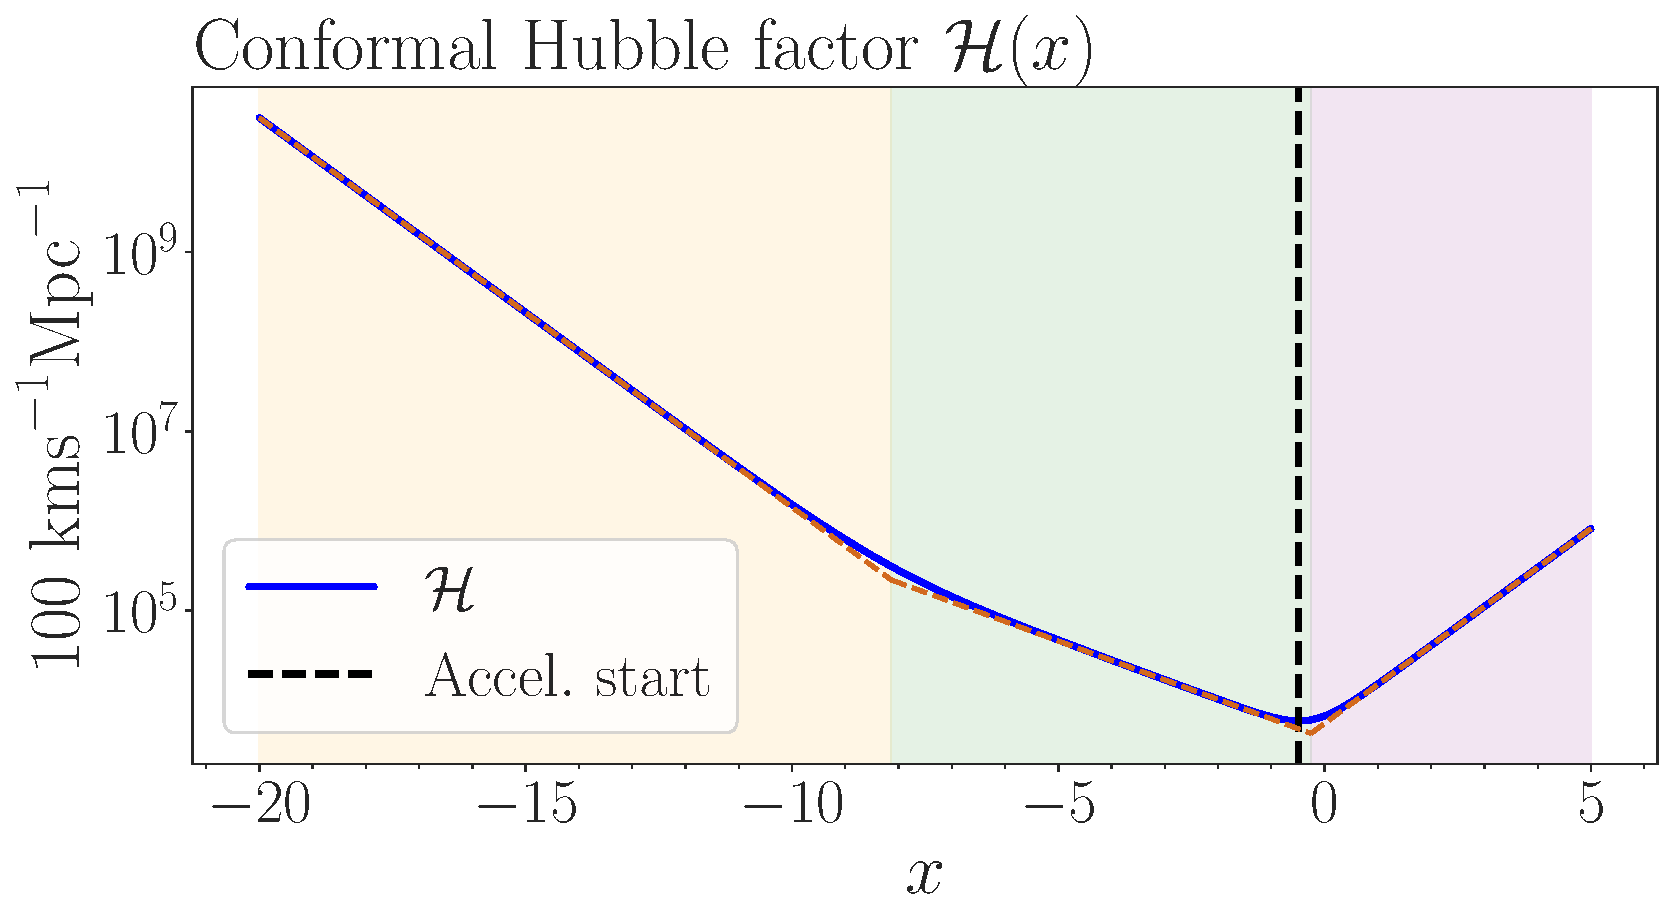
\includegraphics[width=\linewidth]{conformal_hubble_factor.pdf}
        \caption{$\Hp$ as function of $x$. It is decreasing in the radiation and matter regimes, and increasing in the dark energy regime, tightly following its analytical approximation in each regime.}
        \label{fig:m1:conformal_hubble_factor_Hp}
    \end{figure}

    ~\cref{fig:m1:cosmic_conformal_time} show the cosmic time $t$ and the conformal time $\eta/c$. The cosmic time is the age of the universe at any given time/size $x$. The low values for the cosmic time at early times suggest a rapid increase of the size of the Universe in a short cosmic time. This is supported by the conformal Hubble factor in ~\cref{fig:m1:conformal_hubble_factor_Hp} which is large for low $x$. The expansion rate of the universe decelerates until the acceleration onset, from which it accelerates. \TODO{explain $\eta$ and $t$ more}

    \begin{figure}
        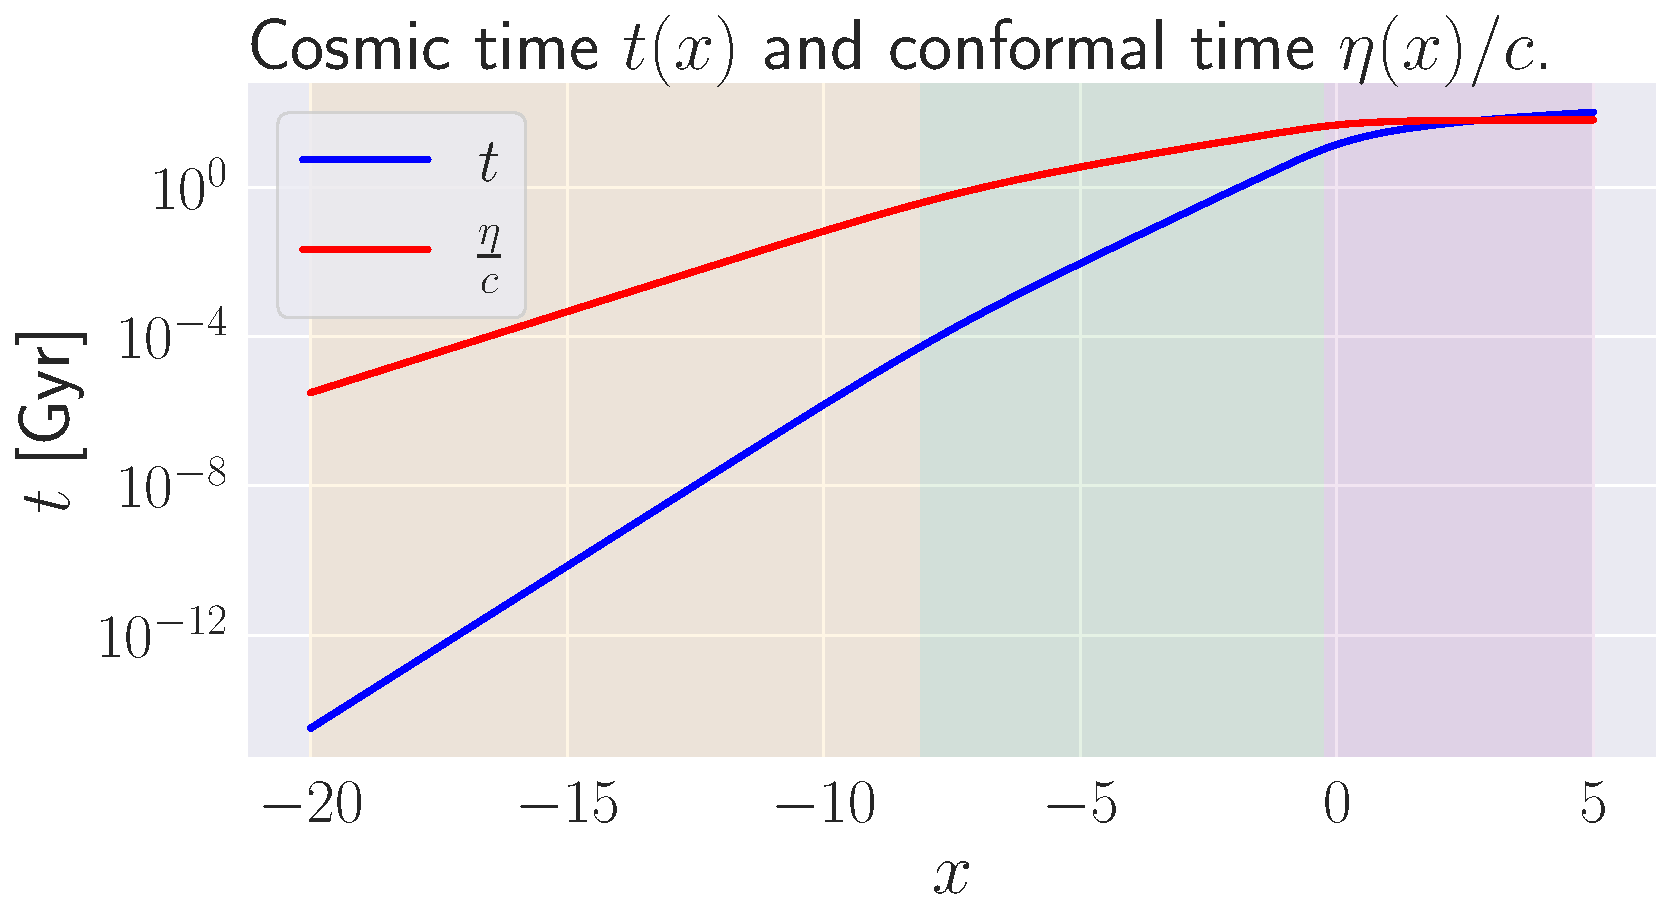
\includegraphics[width=\linewidth]{cosmic_conformal_time.pdf}
        \caption{Cosmic time (in blue) and conformal time (red). \TODO{find meaning behind this plot}.}
        \label{fig:m1:cosmic_conformal_time}
    \end{figure}

    The results of the supernova fitting, outlined in section ~\cref{sec:m1:methods:fit}, is summarised in ~\cref{tab:m1:best_fit_values}. The parameter values that maximises the likelihood (minimising) $\chi^2$ are: $h=0.702$, $\O_\mathrm{M0} = 0.259$ and $\O_{k0} = 0.274$. We also compute the posterior probability distribution function obtained from ~\cref{eq:m1:methods:fit:posterior_prob} which we have assumed to be normally distributed. From this we obtain a mean value, but also a $1\sigma$ confidence interval, which is:
    \begin{equation}\label{eq:m1:results:posterior_results}
        \begin{split}
            h &= 0.701\pm0.006 \\
            \O_\mathrm{M0} &= 0.247\pm0.110 \\
            \O_{k0} &= 0.107 \pm 0.274
        \end{split}
    \end{equation}
    \TODO{cont.}
    \begin{table}
        \begin{tabular}{l|rrr}
      & $h$ & $\O_\mathrm{M0}$ & $\O_{k0}$  \\
    \hline
    Best: $\min{\chi^2}$  & 0.702 & 0.259 & 0.067  \\
    Posterior  & 0.701 & 0.247 & 0.107   \\
    $1\sigma$ confidence  & 0.006 & 0.110 & 0.274 \\ 
    \hline
    \hline
\end{tabular}
        \caption{Best and fitted values. The best fit values are those that actually minimise the $\chi^2$-value, which consequently are the most probable values. The fitted values are obtained as the mean and standard deviations of the posterior pdfs of the parameters respectively. }
        \label{tab:m1:best_fit_values}
    \end{table}

    ~\cref{fig:m1:supernova_data} shows the supernova data as red error bars, with the predictions from the fiducial cosmology plotted above it, alongside the best fit parameter values. The quantity plotted is the luminosity distance divided by redshift, $d_L/z$ for better comparison. We notice the accordance between the two, and also note that the $x$-axis in this plot is the redshift $z$ instead of the logarithm of the scale factor. This means that earlier times are to the right in the plot (high redshift), as opposed to the other plots. 

    \begin{figure}
        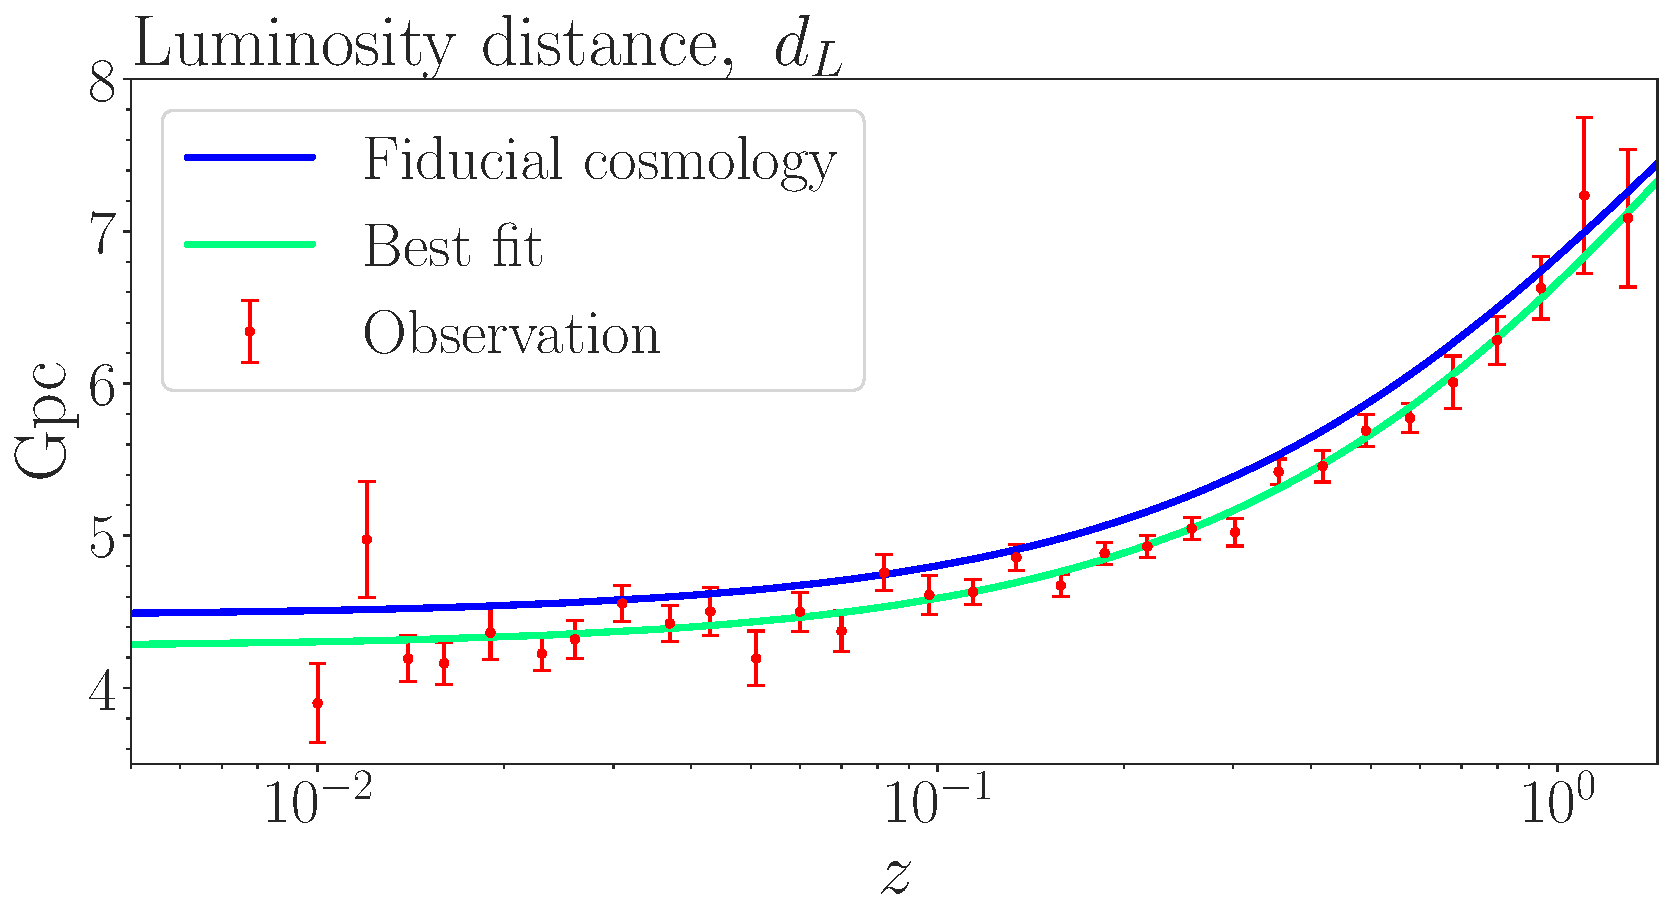
\includegraphics[width=\linewidth]{supernova_data.pdf}
        \caption{The luminosity distance predicted using the fiducial cosmology in blue, against observations of actual supernovas in red (or rather the confidence interval of the observations). The green line is found from computing the luminosity distance using a cosmology of the best fit parameters from the supernova fitting; $h=0.702, \O_\mathrm{b0} = 0.05, \O_\mathrm{CDM0} = 0.209, \O_\mathrm{k}=0.067, N_\mathrm{eff}=3.046, T_\mathrm{CMB}=2.7255 \text{K}$. Notice the $x$-axis is now the redshift $z=e^x-1$.}
        \label{fig:m1:supernova_data}
    \end{figure}

    \begin{figure}
        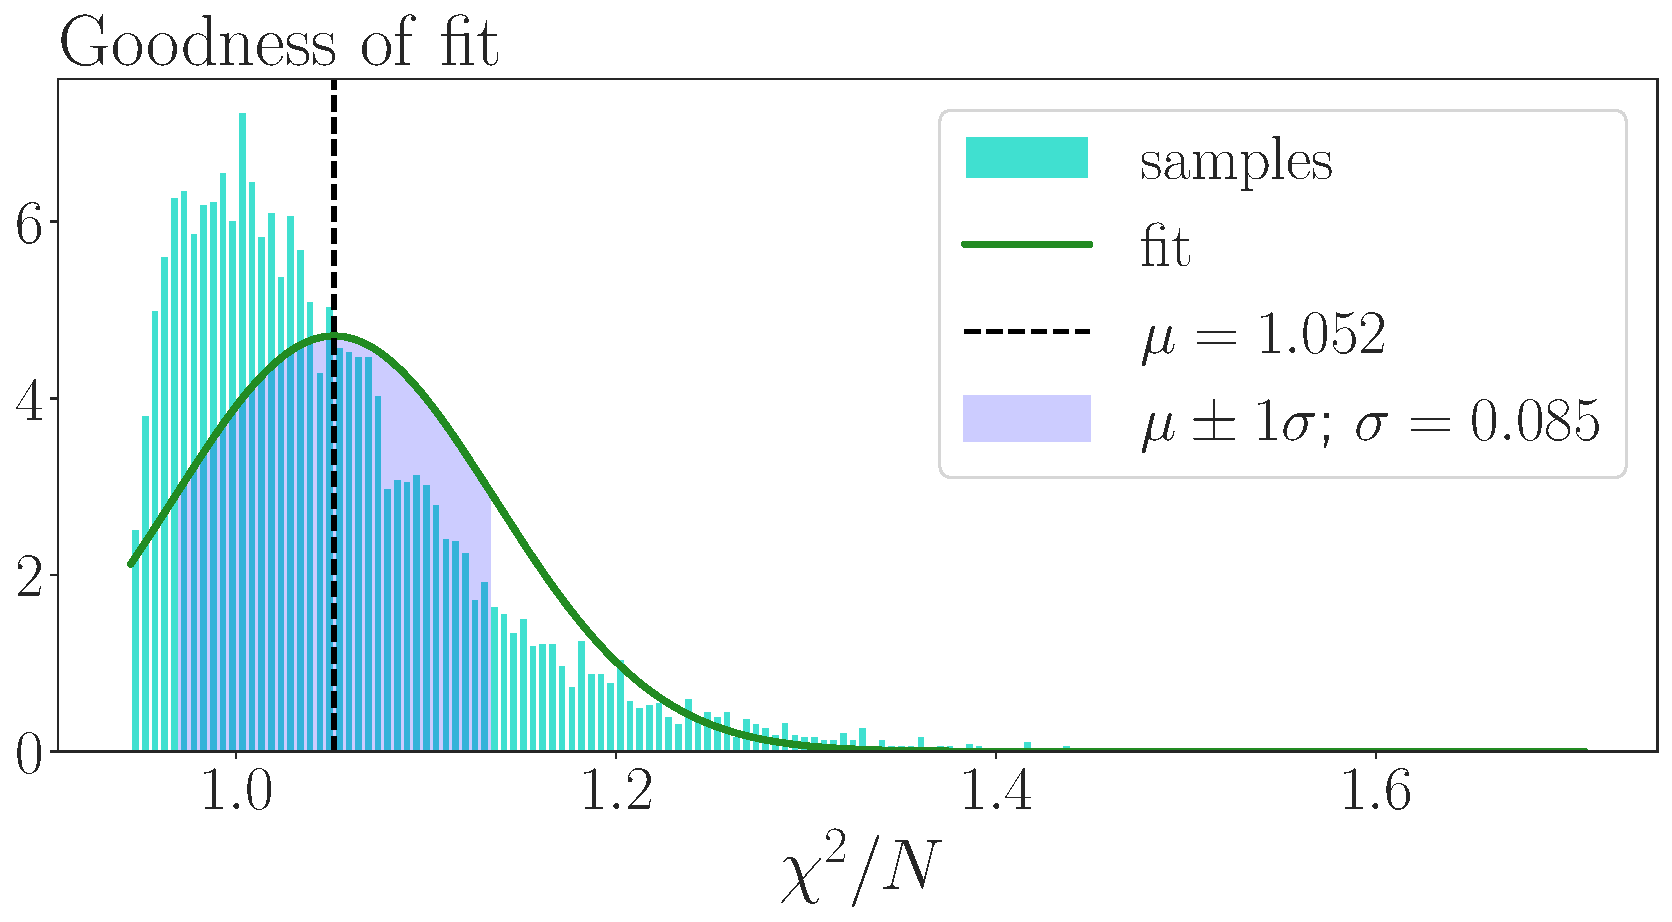
\includegraphics[width=\linewidth]{goodnes_of_fit.pdf}
        \caption{Goodness of fit}
        \label{fig:m1:goodness_of_fit}
    \end{figure}

    \cref{fig:m1:omega_planes} shows the $\chi^2$-values found from \cref{eq:m1:chi2_test_def}, to 1$\sigma$ accuracy. The black dotted line represent a flat universe, where the matter and dark energy are the main constituents of the universe. The supernova data originate in close temporal proximity to us, we thus assume that the contribution from the radiation density is negligible for making constraints on $\O_\mathrm{M}$ and $\O_\Lambda$ today. 

    \begin{figure}
        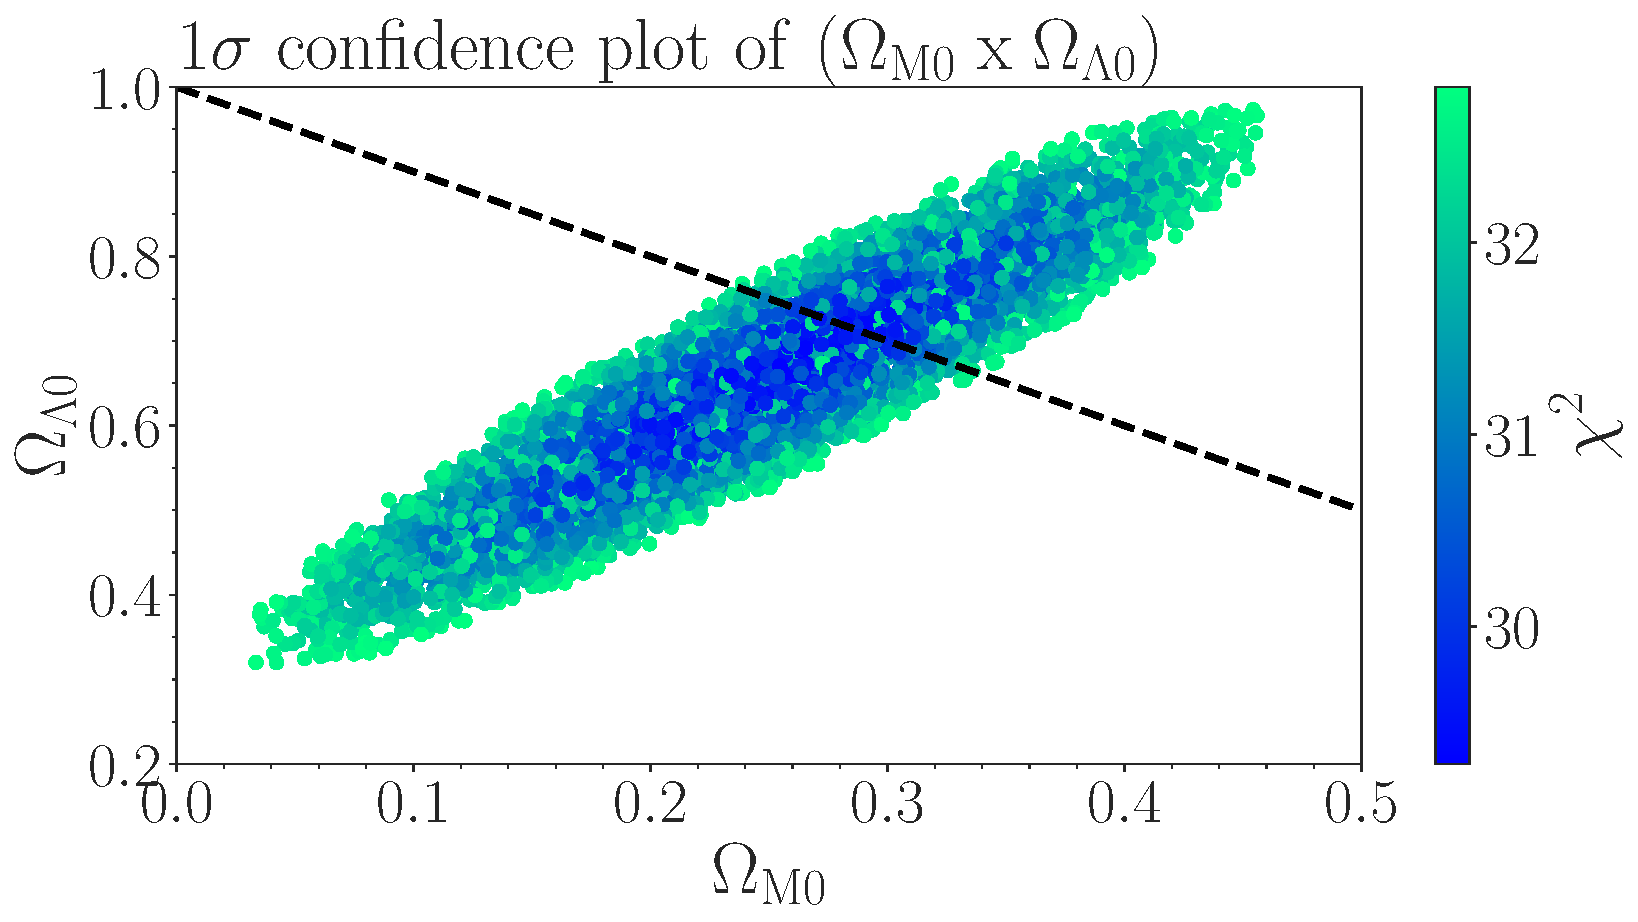
\includegraphics[width=\linewidth]{omega_plane.pdf}
        \caption{Scatter plot showing the $chi^2$-error of the luminosity distance $d_L$ between the observed values and the prediction, as function of $\O_\mathrm{M}$ and $\O_\Lambda$. The data shown is within $1\sigma$ (standard deviation). The black dotted line signifies a flat universe. }
        \label{fig:m1:omega_planes}
    \end{figure}

    The MCMC method allow us to make a posterior probability distribution of the parameters in question. \cref{fig:m1:posterior_pdf_H0} the distribution of the Hubble factor $H_0$ constructed from the sampled values of $h$. The actual samples are shown in green and the corresponding fitted probability distribution in blue. 


    \begin{figure}
        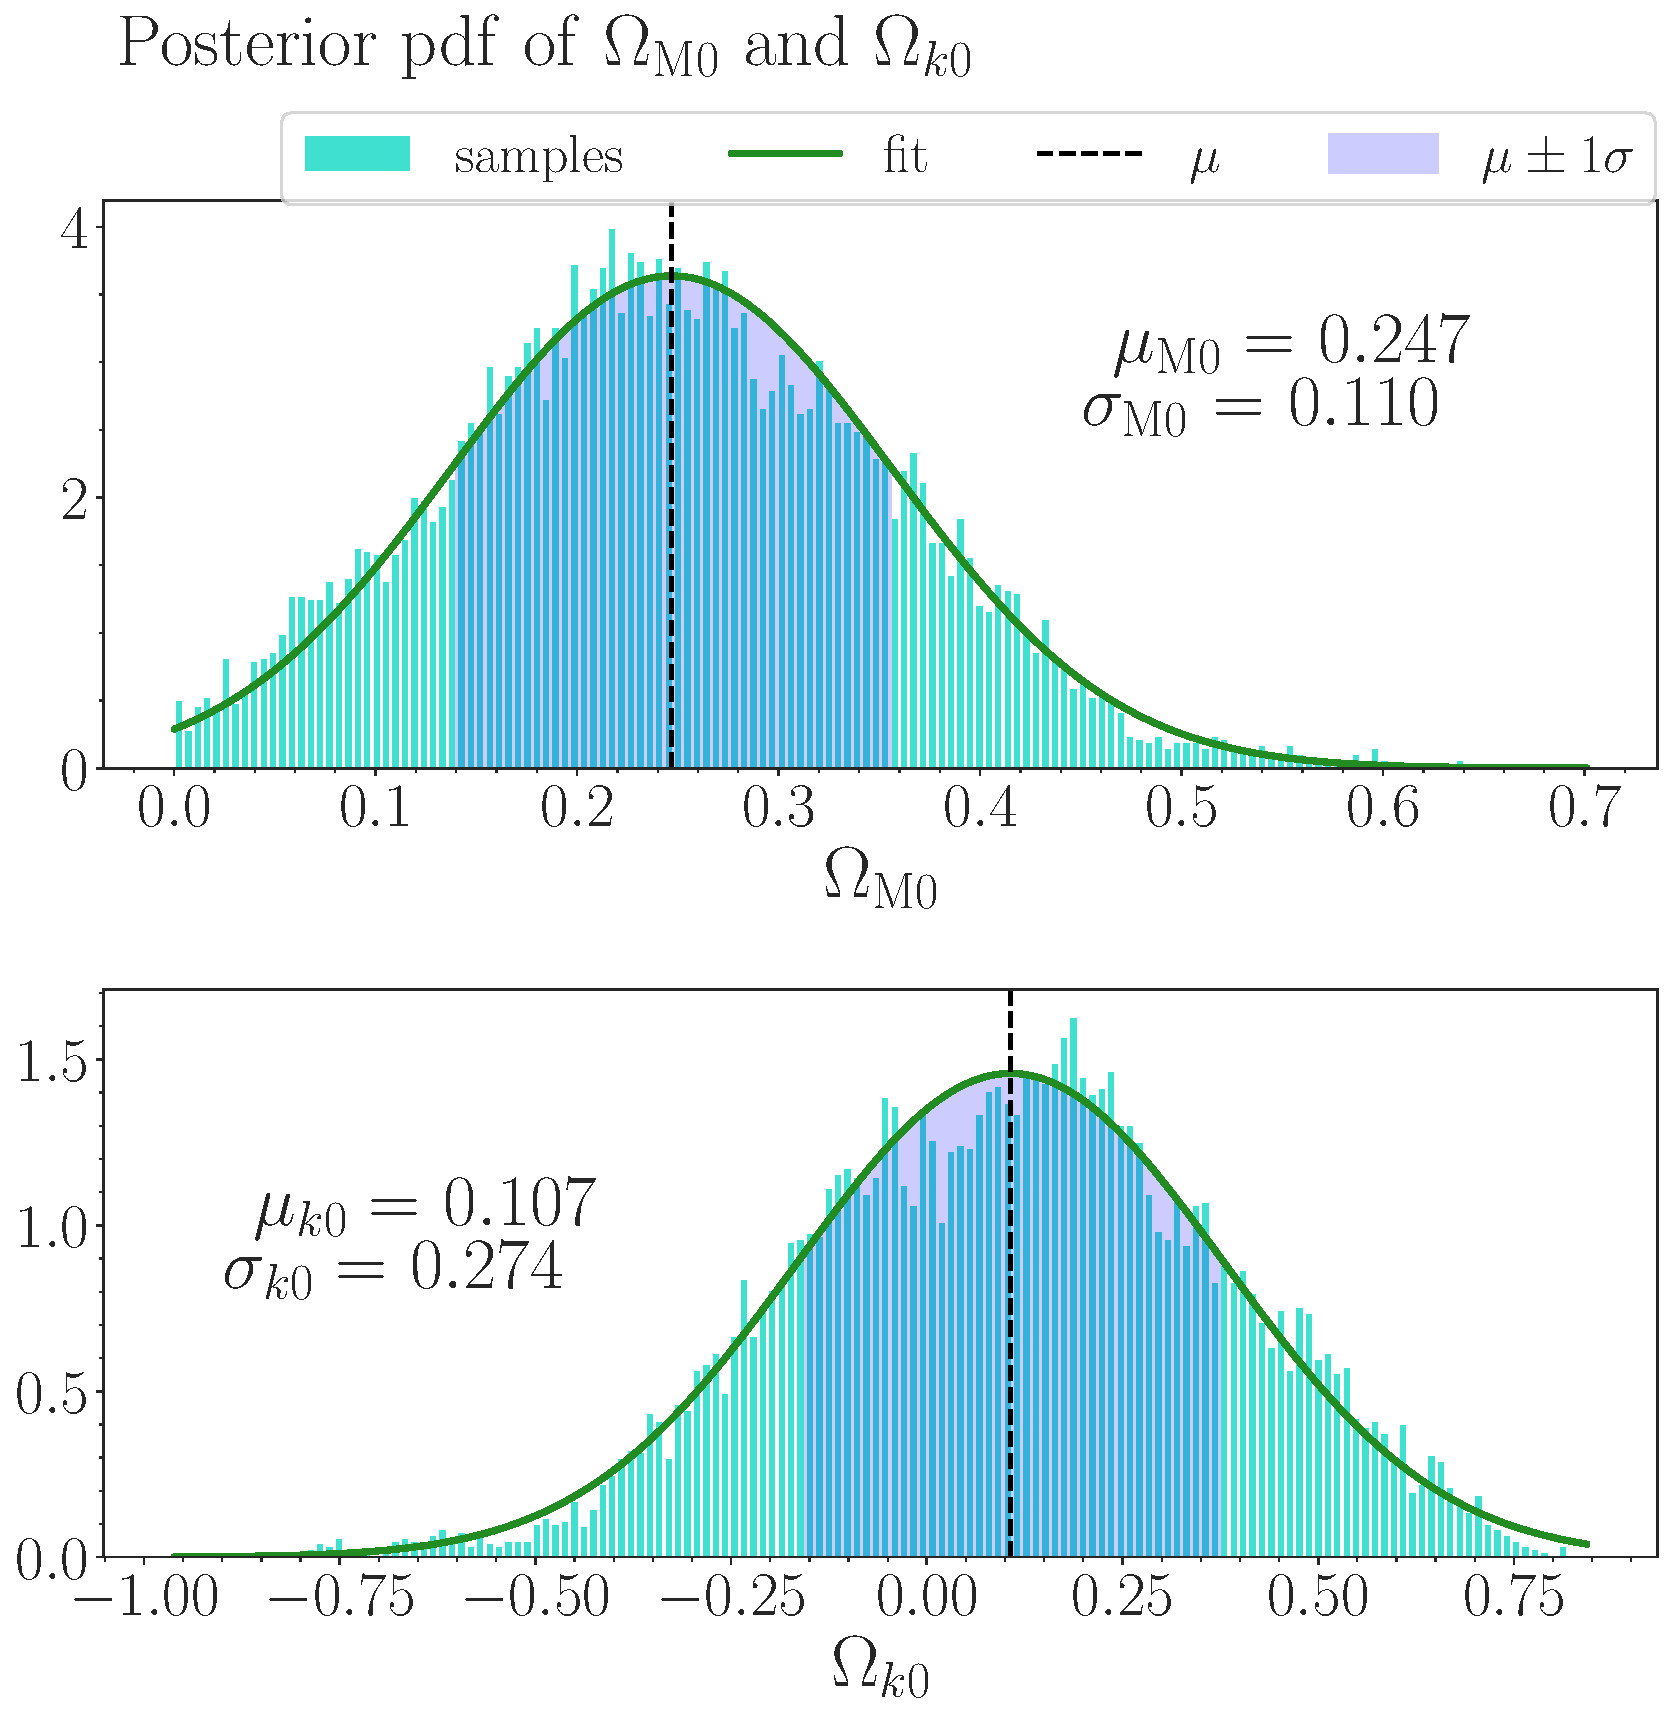
\includegraphics[width=\linewidth]{probs_M_K.pdf}
        \caption{Posterior probability distributions (pdfs) of $\O_mathrm{M}$ and $\O_\mathrm{k}$ as result of the MCMC sampling. The samples as shown in turquoise and the constructed pdfs in green. The mean $\mu$ is shown as a black dotted line, with the $1\sigma$ confidence interval in shaded blue ($\mu\pm 1\sigma$)}
        \label{fig:m1:posterior_pdf_omega_m_k}
    \end{figure}

    \begin{figure}
        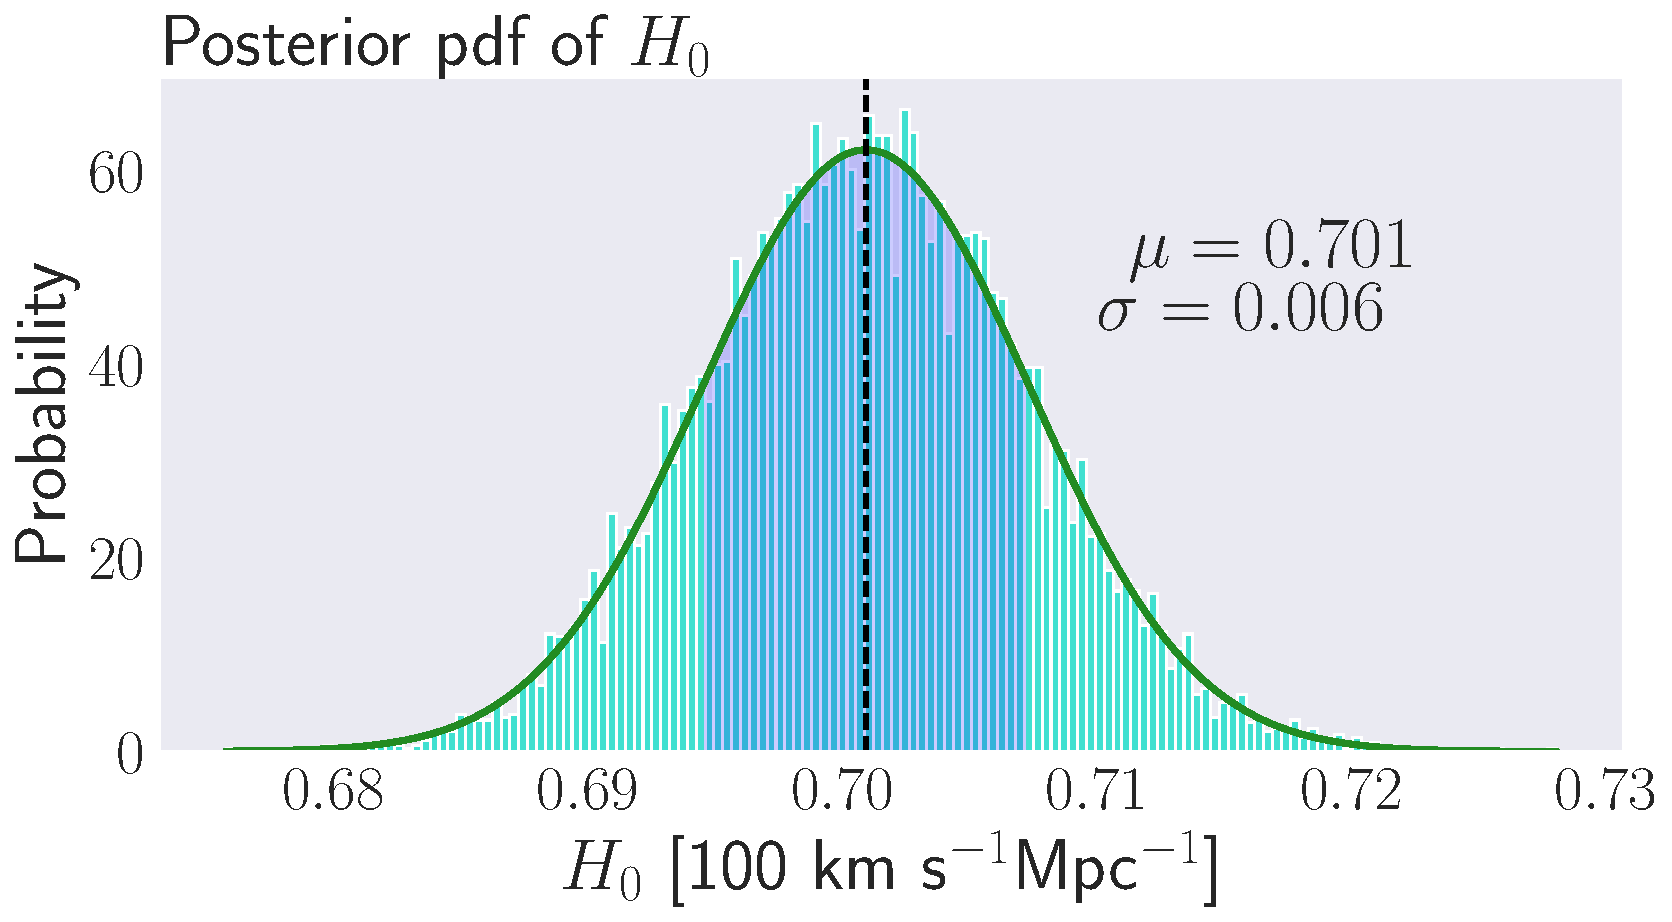
\includegraphics[width=\linewidth]{posterior_pdf.pdf}
        \caption{Posterior probability distribution (pdf) of $H_0$ as result of the MCMC sampling.}
        \label{fig:m1:posterior_pdf_H0}
    \end{figure}


\section{Milestone II}\label{sec:m2}

Some introduction to milestone 2

\subsection{Theory}\label{sec:m2:theory}
    In order to explain the inventory of the universe, we need to understand how the distribution of different species changes over time. This is governed by the \textit{Boltzmann equation},
    \begin{equation}\label{eq:m2:theory:bolzmann_def}
        \dv{f}{t} = C[f],
    \end{equation}
    where $f(\vec{x},\vec{p},t)$\footnote{Given in \textit{phase-space coordinates}: ($x^\mu,P^\mu$)} is the distribution function of a given species. $C[f]$ are the collision terms, which depends on the species through the same distribution function $f$. Due to the function dependencies of $f$ we are able to generally expand it into ~\cite[Eq. 3.33]{dodelson2020modern}:
    \begin{equation}\label{eq:m2:theory:bolzmann_expanded}
        \dv{f}{t} = \pdv{f}{t}+\pdv{f}{x^i}\dv{x^i}{t} + \pdv{f}{p}\dv{p}{t} + \pdv{f}{\hat{p}^i}\dv{\hat{p}^i}{t} = C[f],
    \end{equation}
    where $p=\abs{\vec{p}}$ and $\hat{p}=\vec{p}/p$.

    Before recombination, the equilibrium between protons, electrons and photons is governed by the following interaction, from ~\cite{weinberg2008cosmology}\footnote{Where $H^*$ denotes excited states of hydrogen which will decay into neutral hydrogen.}:
    \begin{equation}\label{eq:m2:theory:equilibrium_interaction}
        e^-+p^+\leftrightharpoons H^* + \gamma,
    \end{equation}
    where a proton and an electron interact to form an excited hydrogen atom, which decays and emits a photon, or a photon excites and split a hydrogen atom into a free electron and a proton through \textit{Compton scattering}.\footnote{Elastic scattering of photons is technically Thomson scattering, but Compton scattering is a more general term and will be used (~\cite{dodelson2020modern}). This is also why we later use the Thomson cross section $\sigma_T$. The reaction is when a photon scatters of an electron, and possibly energises it enough to break out of the hydrogen atom, if already bound: $$\gamma + e^- \leftrightharpoons \gamma+e^-.$$} ~\cref{eq:m2:theory:equilibrium_interaction} is a reaction of the form $1+2\leftrightharpoons 3+4$, and we have from ~\cite{AST5220LectureNotes} that the Boltzmann equation for such a reaction is:
    \begin{equation}\label{eq:m2:theory:boltzmann_eq}
        \frac{1}{n_1e^{3x}}\dv{(n_1e^{3x})}{x} = -\frac{\Gamma}{H}\left(1-\frac{n_3n_4}{n_1n_2}\left(\frac{n_1n_2}{n_3n_4}\right)_\mathrm{eq}\right),
    \end{equation}
    where $n_i$ are the number densities of the reactants, $\Gamma$ is the reaction rate and $H$ the Hubble parameter (expansion rate of the universe). If the reaction rate is much larger than the expansion rate of the universe, $\Gamma \gg H$, then ~\cref{eq:m2:theory:equilibrium_interaction} ensures equilibrium between protons, electron and photons. When $\Gamma$ drops below $H$, then the expansion rate becomes dominant and the reaction rate is unable to sustain equilibrium. This happens when the temperature of the Universe becomes lower than the binding energy of hydrogen, hence stable neutral hydrogen is able to form.\footnote{Well, it is really not as simple, as neutral hydrogen is obtained from excited hydrogen and how this process go about is non-trivial. As we ignore re-ionisation, I will not delve into this. However, both ~\cite[p. 113-129]{weinberg2008cosmology}, ~\cite[p. 95-99]{dodelson2020modern} and ~\cite{AST5220LectureNotes} elaborate further on this.} As a consequence, the photons \textit{decouple} from the protons and electron. When $\Gamma \ll H$, there are practically no interactions and the number density becomes constant for a comoving volume. Massive particles \textit{freeze out} and their abundance become constant. 

\subsubsection{Hydrogen recombination}\label{sec:m2:theory:hydrogen_recombination}
    We express the electron density through the free electron fraction $X_e \equiv n_e/n_\mathrm{H} = n_e/n_b$ where we have assumed that hydrogen make up all the baryons ($n_b=n_\mathrm{H}$). We also ignore the difference between free protons and neutral hydrogen. From ~\cite{https://doi.org/10.48550/arxiv.astro-ph/0606683} we obtain:
    \begin{equation}\label{eq:m2:theory:baryon_number_density}
        n_b = \frac{\rho_b}{m_\mathrm{H}} = \frac{\O_b\rho_c}{m_\mathrm{H}}\expe{-3x},
    \end{equation}
    where $m_\mathrm{H}$ is the mass of the hydrogen atom, and $\rho_c$ the critical density today as defined earlier. Before recombination, no stable neutral hydrogen is formed, thus the electron and baryon density is the same, i.e. there are only free electrons so $X_e \simeq 1$. When in equilibrium, the r.h.s. of ~\cref{eq:m2:theory:boltzmann_eq} reduces to 0, which is called the \textit{Saha approximation}. The solution is in this regime described by the \textit{Saha equation}, which from ~\cite{dodelson2020modern} in physical units is:
    \begin{equation}\label{eq:m2:theory:Saha_equation}
        \frac{X_e^2}{1-X_e} = \frac{1}{n_b}\left(\frac{k_Bm_eT_b}{2\pi\hbar^2}\right)^{3/2}\expe{-\epsilon_0/k_BT_b},
    \end{equation}
    where $\epsilon_0 = 13.6\text{ eV}$ is the ionisation energy of hydrogen. The Saha equation is only a good approximation when $X_e \simeq 1$. Thus for $X_e < (1-\xi)$,\footnote{Where $\xi$ is some small tolerance, which have to be defined in some numerical model for when to abonden the Saha equation and use the more accurate, but computationally more expensive Peebles equation. This is typically $\xi=0.001$} which corresponds to the period during and after recombination, we have to make use of the more accurate \textit{Peebles equation}. From ~\cite{https://doi.org/10.48550/arxiv.astro-ph/0606683}:
    \begin{subequations}\label{eq:m2:theory:peebles_equation}
        \begin{equation}
            \dv{X_e}{x} = \frac{C_r(T_b)}{H}\left[\beta(T_b)(1-X_e)-n_\mathrm{H}\alpha^{(2)}(T_b)X_e^2\right],
            \tag{\ref{eq:m2:theory:peebles_equation}}
        \end{equation}
        where
        \begin{align}
                C_r(T_b) &= \frac{\Lambda_{2s-1s}+\Lambda_\alpha}{\Lambda_{2s-1s} + \Lambda_\alpha+\beta^{(2)}(T_b)},\label{eq:m2:theory:peebles_CR} \\
                \Lambda_{2s-1s} &= 8.227 \unit{s}^{-1}, \label{eq:m2:theory:peebles_lambda}\\
                \Lambda_\alpha &= \frac{1}{(\hbar c)^3}H\frac{(3\epsilon_0)^3}{(8\pi)^2n_{1s}}, \label{eq:m2:theory:peebles_lambda_alpha}\\
                n_{1s} &=(1-X_e)n_\mathrm{H}, \label{eq:m2:theory:peebles_ns}\\
                n_\mathrm{H} &= (1-Y_p)\frac{3H_0^2\O_{b0}}{8\pi Gm_\mathrm{H}}\expe{-3x}, \label{eq:m2:theory:peebles_nH}\\
                \beta^{(2)}(T_b) &= \beta(T_b)\expe{3\epsilon_0/4k_BT_b}, \label{eq:m2:theory:peebles_beta2}\\
                \beta(T_b) &= \alpha^{(2)}(T_b)\left(\frac{k_Bm_eT_b}{2\pi\hbar^2}\right)^{3/2}\expe{-\epsilon_0/k_BT_b}, \label{eq:m2:theory:peebles_beta}\\
                \alpha^{(2)}(T_b) &=\frac{\hbar^2}{c}\frac{64\pi}{\sqrt{27\pi}}\frac{\alpha^2}{m_e^2}\sqrt{\frac{\epsilon_0}{k_BT_b}}\phi_2(T_b), \label{eq:m2:theory:peebles_alpha}\\
                \phi_2(T_b) &= 0.448\ln\left(\frac{\epsilon_0}{k_BT_b}\right). \label{eq:m2:theory:peebles_phi2}
        \end{align}
    \end{subequations}

    The Peebles equation takes into account that the energy (excitation) of hydrogen formed through ~\cref{eq:m2:theory:equilibrium_interaction} vary, and that decays take place until we reach the $n=2$ level (first excited state), denoted by $^{(2)}$ in ~\cref{eq:m2:theory:peebles_CR}-~\cref{eq:m2:theory:peebles_phi2}. Recombination to the ground state is not relevant, as this leads to an ionised photon which immediately ionises a neutral hydrogen atom ~\cite[p. 97]{dodelson2020modern}. The $C_r$ is the probability that singly ionised hydrogen is reionised further, where $\beta^{(2)}$ and $\beta$ are the collisional ionisations from the first ionised state and ground state respectively. $\alpha^{(2)}$ is the recombination rate to excited states. For more detailed description of these terms, see ~\cite{Ma_1995}. \footnote{Because of this non-trivial path into the ground state, and the large photon to baryon number ratio, recombination happens later than when the temperature of the universe correspond to exactly the binding energy of neutral hydrogen (~\cite{https://doi.org/10.48550/arxiv.astro-ph/0606683})}

    We find $X_e$ by solving ~\cref{eq:m2:theory:Saha_equation} for $X_e > (1-\xi)$ and ~\cref{eq:m2:theory:peebles_equation} for $X_e < (1-\xi)$. In theory, it is possible to solve the Peebles equation at very early times, but the equation is very stiff resulting in unstable numerical solutions at early times (high temperatures), hence the Saha approximation.

\subsubsection{Visibility}\label{sec:m2:theory:visibility}
    Visibility is a concept tied to the optical depth and mean free path of a medium. The two latter are inversely proportional to each other. The mean free path is the average distance a photon travels before its direction is changed (often by scattering). Thus, a small mean free path gives results in a lot of collision across short distances, which occurs in optically thick media. The optical depth as a function of conformal time is defined as \cite{AST5220LectureNotes}:
    \begin{equation}\label{eq:m2:theory:optical_depth}
        \tau = \int_\eta^{\eta_0} n_e\sigma_\mathrm{T}\expe{-x}\d\eta',
    \end{equation}
    where $n_e$ is the electron density and $\sigma_\mathrm{T}$ is the Thompson cross-section. In differential form, restoring original units, this is:
    \begin{equation}\label{eq:m2:theory:optical_depth_differential}
        \dv{\tau}{x} = -\frac{cn_e\sigma_Te^x}{\Hp}.    
    \end{equation} 
    From this we define the visibility function, $g$:
    \begin{equation}\label{eq:m2:theory:visibility_function}
        \begin{split}
            g &= -\dv{\tau}{\eta}\expe{-\tau} = -\Hp\dv{\tau}{x}\expe{-\tau}\\
            \tilde{g} &\equiv -\dv{\tau}{x}\expe{-\tau} = \frac{g}{\Hp},
        \end{split}
    \end{equation}
    where $\tilde{g}$ is in terms of the preferred time variable, $x$. Notable thing about the visibility function $\tilde{g}$ is that it is a true probability distribution, describing the probability density of some photon to last have scattered at time $x$. Because of this, we have that $\int_{-\infty}^0\tilde{g}(x)\d x = 1$. We also take note of the derivative of the visibility function:
    \begin{equation}\label{eq:m2:theory:visibility_function_deriv}
        \dv{\tilde{g}}{x} = e^{-\tau}\left[\left(\dv{\tau}{x}\right)^2-\dv[2]{\tau}{x}\right]
    \end{equation}


\subsubsection{Sound horizon}
    Let's take a small step back and consider the situation of the early Universe. Before any decoupling, the photons and electrons are coupled through Thompson scattering, and protons and electrons are coupled through coulomb interactions. Because of this, photons interact with baryons and move alongside with them as one fluid, in which wave propagates with a speed $c_s$, from ~\cite{dodelson2020modern}:
    \begin{equation}\label{eq:m2:theory:sound_speed}
        c_s \equiv c\left[3(1+R)\right]^{-\frac{1}{2}} \quad ; \quad R\equiv\frac{3\O_b}{4\O_\gamma},
    \end{equation}
    where $R$ is the \textit{baryon-to-photon energy ratio}. By the definition of $R$, if the baryon density is negligible compared to the radiation density, $R\sim0$, and we recover the wave propagation speed in a relativistic fluid: $c_s=3^{-1/2}$ (~\cite{dodelson2020modern}). The total distance such a wave would have travelled in a time $t$ (since the beginning of the Universe) is called the \textit{sound horizon}, found by simply integrating $c_s$ through time, accounting for the expansion of space itself by including a factor $e^{-x}$:
    \begin{equation}\label{eq:m2:theory:sound_horizon_def}
        s = \int_0^tc_se^{-x}\d t = \int_{-\infty}^x\frac{c_s}{\Hp}\d x,
    \end{equation}
    where the variables are changed to $x$. On differential form:
    \begin{equation}\label{eq:m2:theory:sound_horizon_differential}
        \dv{s}{x} = \frac{c_s}{\Hp},
    \end{equation}
    which is a straightforward differential equation to solve given some initial conditions. 
\subsection{Methods}\label{sec:m2:methods}

some methods
\subsection{Results and discussion}\label{sec:m2:results} 

    \subsubsection{Times and sound horizon}
    The relevant times for last scattering, recombination and Saha recombination are obtained as explained in ~\cref{sec:m2:methods:analysis}, and presented in ~\cref{tab:m2:recomb_analysis}. These times are given in terms of $x$, the redshift $z$ and the cosmic time $t$ (in Myr). The sound horizon is given in units of megaparsecs (Mpc). Last scattering occurred when $x=-6.9853$, at redshift $z=1079.67$, which is slightly after recombination when $x=-6.9855$ at redshift $z=1079.83$. If the Saha approximation was valid when the electron fraction dropped, recombination would have happened when $x=-7.1404$ at redshift $1260.89$ which is significantly earlier. However, this is not the case since photons drop out of equilibrium with the primordial plasma as soon as hydrogen begin to form, and the free electron fraction is reduced. Thus, this number may only be used for comparison. Another thing worth noting is the validity of these numbers.
    \begin{table}
        \label{tab:m2:recomb_analysis}
        \begin{tabular}{l|rrrr}
\hline
Phenomenon & $x$ & $z$ & $t$ [Myr] & $r_s$ [Gyr] \\
\hline
Last scattering   & -6.99 & 1082.29 & 0.377 & 55394.8 \\
Recombination     & -6.99 & 1079.83 & 0.378 & 55590.6 \\
Saha              & -7.14 & 1260.89 & 0.291 & 43620.6 \\
\hline
\hline
\end{tabular}

        \caption{The times of last scattering and recombination given in terms of $x$, the redshift $z$, the cosmic time $t$ and the sound horizon $r_s$. Also included is the time of recombination found using the Saha approximation only.}
    \end{table}

    \subsubsection{Free electron fraction}
    ~\cref{fig:m2:electron_fraction} shows the free electron fraction $X_e$ as a function of $x$ found using both the Saha and Peebles equation, as explained in ~\cref{sec:m2:methods:electron_fraction}, in blue. Also shown is the results found from the Saha equation only, which tends to zero a lot faster. This is used for comparison only, as we have already stated that the Saha approximation is only valid for $X_e\simeq 1$. The time of recombination is shown for both cases, which for the Saha approximation happens significantly earlier than what is the actual case. The Peebles solution falls off gradually, and converges towards a constant value, which is the present day abundance of free electrons (freeze out abundance). This is found to be $X_e(x=0) = 0.0002$, shown as a brown dashed line in ~\cref{fig:m2:electron_fraction}.

    Since the Peebles equation is a solution of the Boltzmann equation, it takes into account the particle interaction with changing abundance, after the photons decouple from the primordial plasma. It is thus expected that this will result in a much more gradual fall off of the free electron fraction, just as we observe in ~\cref{fig:m2:electron_fraction}.
    \begin{figure}
        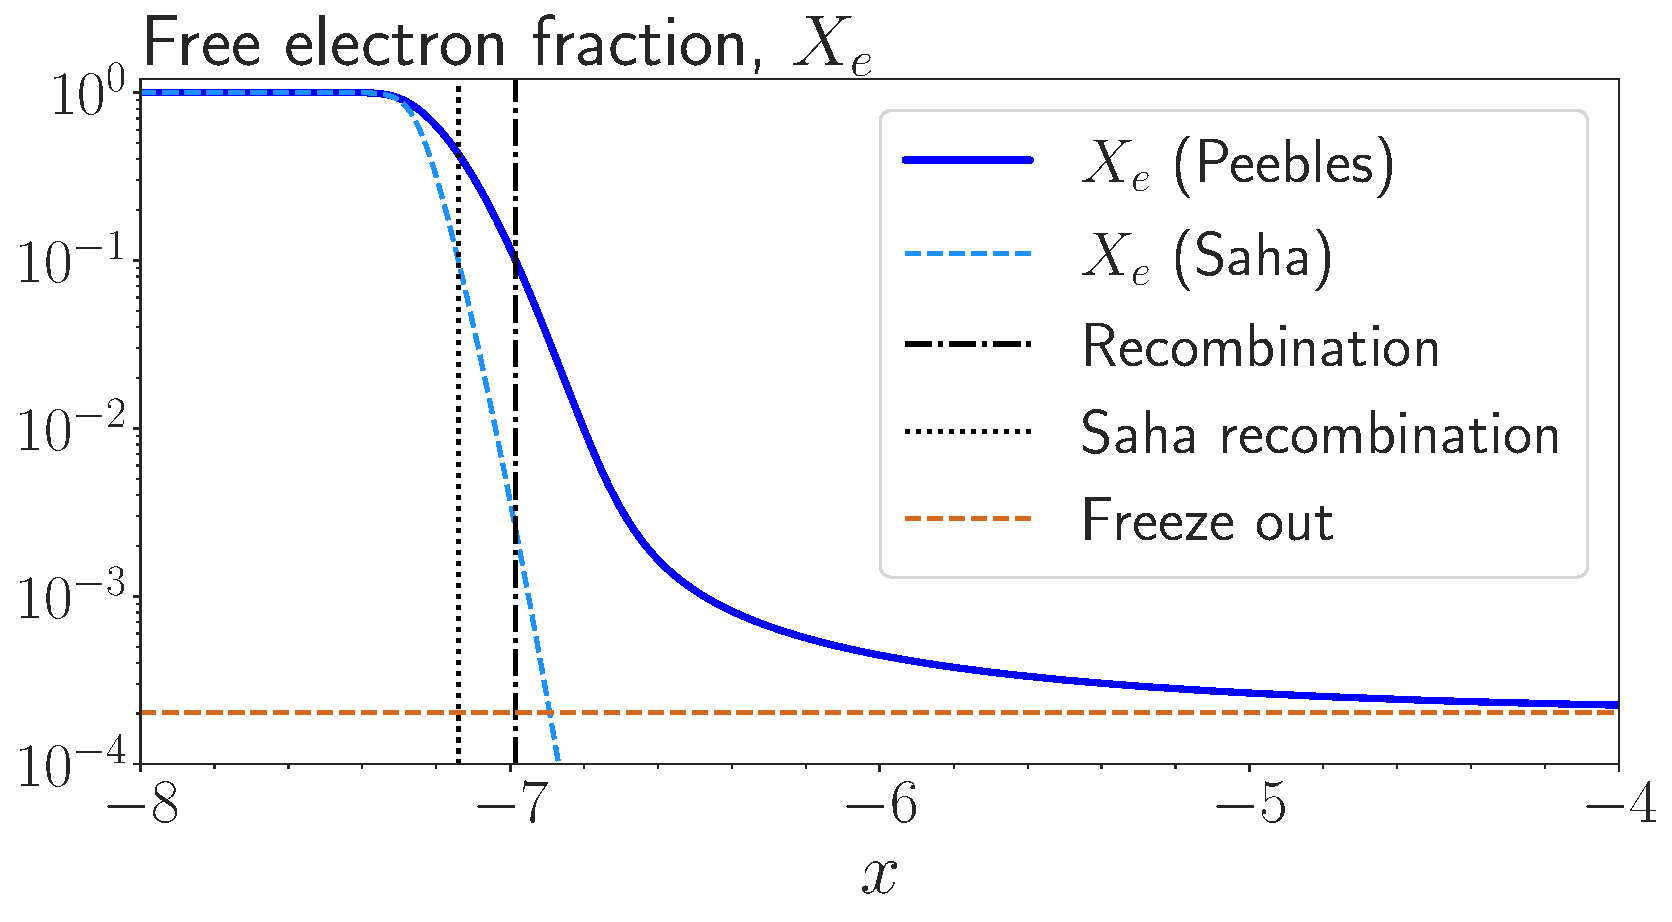
\includegraphics[width=\linewidth]{Xe_plot.pdf}
        \caption{The free electron fraction $X_e$ as function of $x$, found from the Saha and Peebles equation (blue). The result using only the Saha equation is shown in dashed light blue. The time of recombination is shown as a dashed black line. Likewise, recombination in the Saha approximation is shown as a dotted black line, appearing earlier. The freeze out abundance of hydrogen (the present value) is shown as a brown dashed line.}
        \label{fig:m2:electron_fraction}
    \end{figure}

    \subsubsection{Visibility}

    ~\cref{fig:m2:optical_depth} shows the optical depth and its first two derivatives as functions of $x$. This is a function of the time $x$, and thus the optical depth at some value is the integral of ~\cref{eq:m2:theory:optical_depth} from that time until today; it is cumulative. The surface of last scattering is shown with a black dashed line, before which the primordial plasma is optically thick, meaning the photons have a short mean free path. The decrease of the optical depth means that the photons gradually travel longer distances before interacting with free electrons. There are two processes going on here; the expansion of space itself, and the formation of neutral hydrogen. Both of which contribute to the increased mean free path of the photons. The contribution from the expansion of space is slow compared to the seemingly rapid change in the free electron fraction once neutral hydrogen is able to form. Thus, the rapid decrease of free electrons, as seen is ~\cref{fig:m2:electron_fraction} makes the mean free paths of photon to increase beyond the horizon. This effectively enable them to travel through space without interacting with matter, and this is what we observe as the CMB today - the Universe becomes transparent. This sudden decrease of optical depth is clearly seen in ~\cref{fig:m2:optical_depth}, both in $\tau$ itself, but also in its derivatives.
    \begin{figure}
        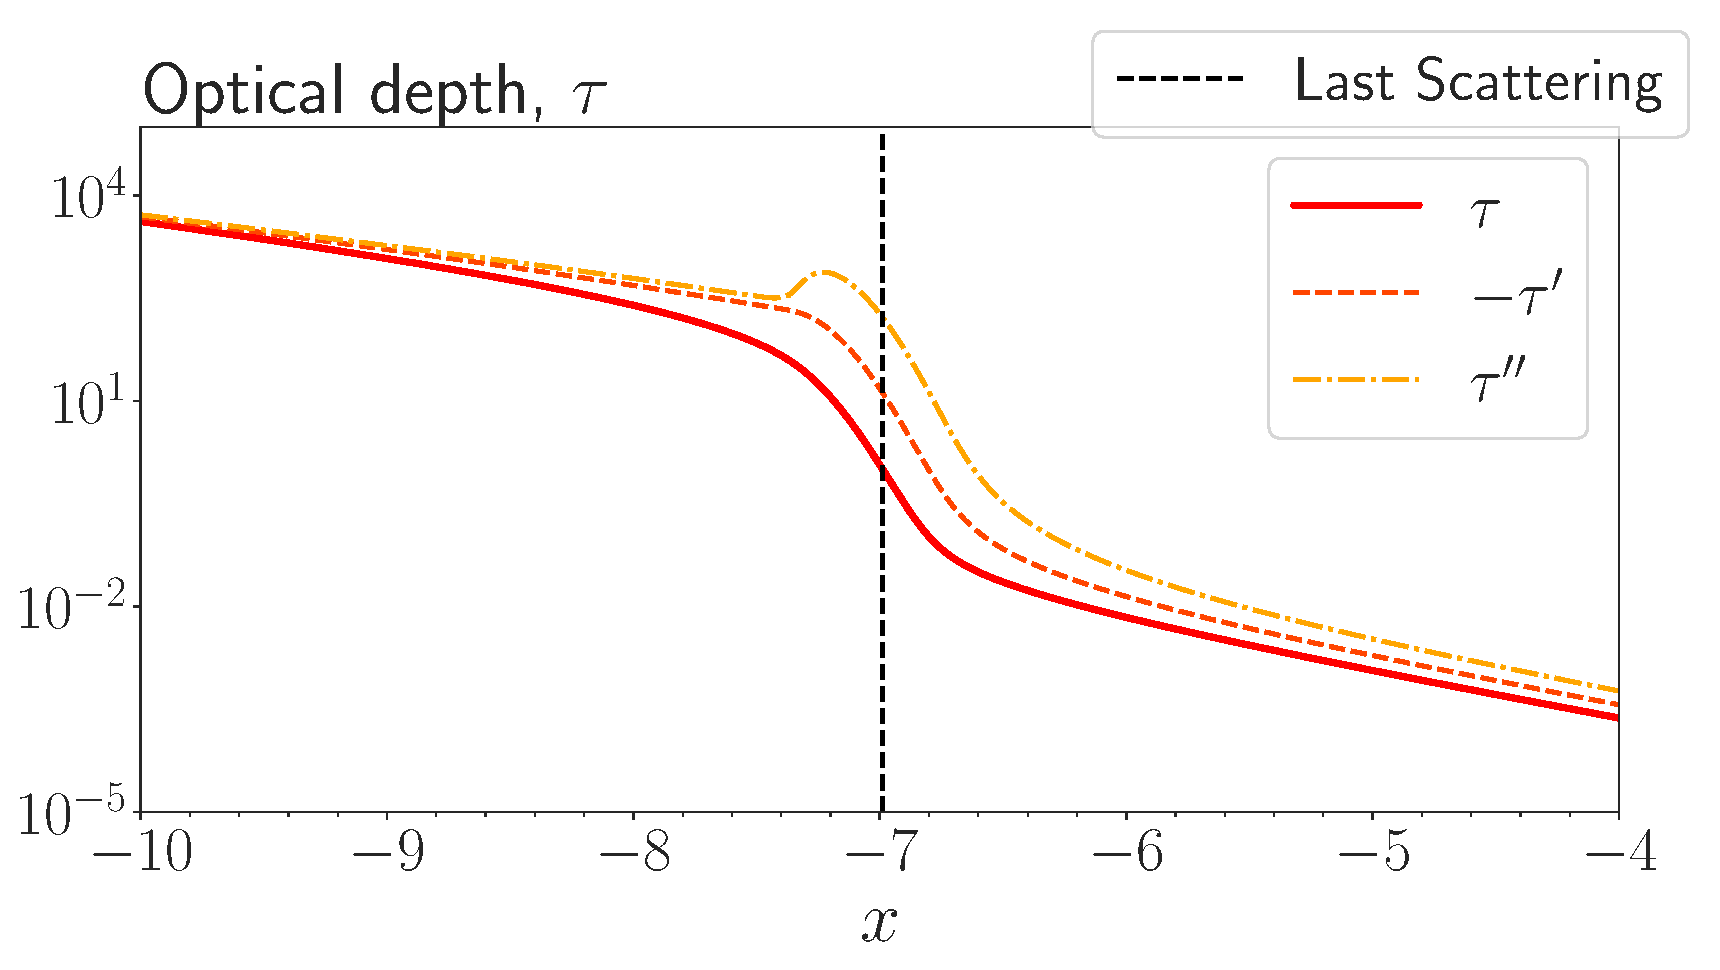
\includegraphics[width=\linewidth]{optical_depth.pdf}
        \caption{The optical depth $\tau$ and its first and second derivatives as functions of $x$. The time of last scattering is shown as a dashed black line, before which the Universe was optically thick.}
        \label{fig:m2:optical_depth}
    \end{figure}

    Another way of arriving at similar conclusions is by considering the visibility function in ~\cref{fig:m2:visibility_function}. Here, $\tilde{g}$ is shown in green along with its derivatives. The scaling follow that of ~\cite{https://doi.org/10.48550/arxiv.astro-ph/0606683}, in order to fit the graphs into the same figure. $\tilde{g}$ describes the probability that a photon reaching us today scattered at time $x$. The peak of this function indicates the time were \textit{the most} photons scattered for the last time, and is thus used as a definition of the last scattering surface. The visibility function is skewed forward in time.
    \begin{figure}
        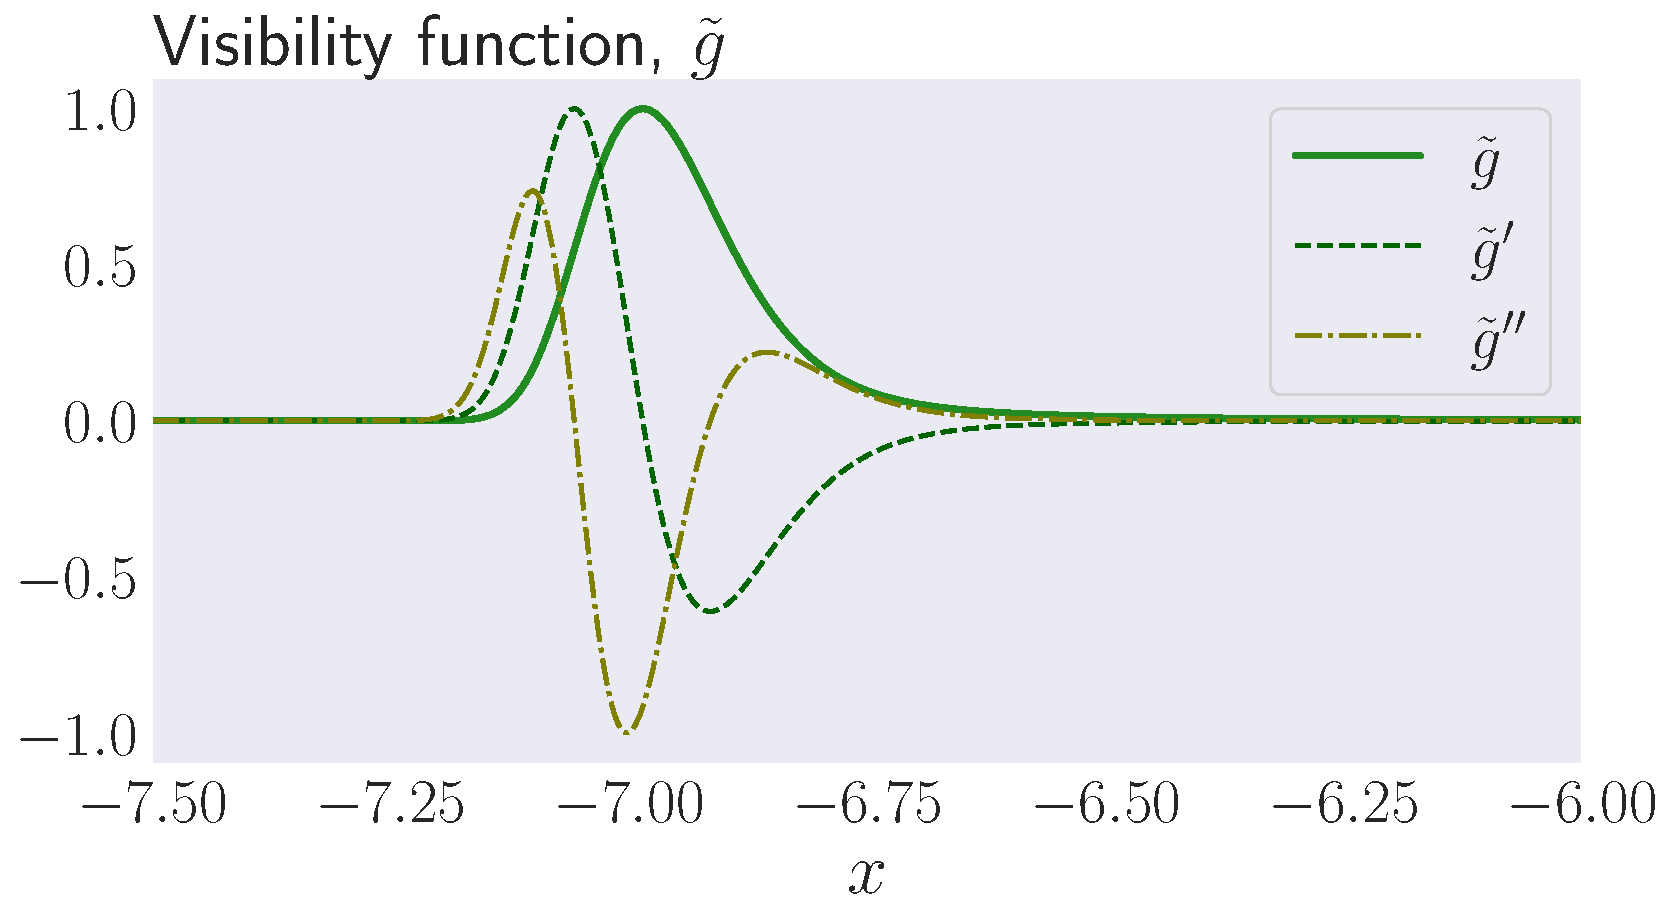
\includegraphics[width=\linewidth]{visibility_function.pdf}
        \caption{The visibility function $\tilde{g}$ and its first and second derivatives as functions of $x$. The time of last scattering is shown as a dashed black line, which by definition coincides with the peak of the visibility function.}
        \label{fig:m2:visibility_function}
    \end{figure}

    \subsubsection{General discussion}
    One key thing to keep in mind is that recombination did not happen instantaneously, but rather over a relatively short period in which neutral hydrogen formed rapidly. This caused a rapid decrease of the free electron fraction, which again caused the optical depth to decrease by several magnitudes. In the same period, we see a that the visibility function is non-zero, meaning the probability of last scattering is (relatively) very high in this period. The times quoted in ~\cref{tab:m2:recomb_analysis} are times that arise from our quite rigid, but fair definition of last scattering and recombination. However, these times do not encapsulate the duration of the abovementioned period.  One could also define the last scattering surface as the time when $\tau=1$ which is the transition between optically thick and optically thin media (when the photon travels exactly one mean free path before scattering). However, the visibility function is arguably a better choice since this is a proper probability distribution, so its peak represents the \textit{actual} time when the probability of last scattering was the highest. Nevertheless, if we change these definitions we ought to expect different times as a result.




\section{Milestone III}\label{sec:m3}

Some introduction to milestone 3

\subsection{Theory}\label{sec:m3:theory}

\subsubsection{Metric perturbations}
    The perturbed metric in the conformal-Newtonian gauge is given in ~\cite{https://doi.org/10.48550/arxiv.astro-ph/0606683} as:
    \begin{equation}\label{eq:m3:theory:perturbed_metric}
        g_\munu = \begin{pmatrix}
            -(1+2\Psi) & 0 \\
            0 & e^{2x}\delta_{ij}(1+2\Phi)
        \end{pmatrix}
    \end{equation}

\subsubsection{Fourier space and multipole expansion}
    Consider a function $f(\vec{x},t)$. Its Fourier transform $\FF$ and inverse $\FF^{-1}$ are defined as:
    \begin{equation}\label{eq:m3:theory:fourier_def}
            \FF[f(\vec{x},t)]  \equiv \frac{1}{(2\pi)^{3/2}}\int e^{-i\vec{k}\cdot\vec{x}}f(\vec{x},t)\d^3 x = \tilde{f}(\vec{k},t),
    \end{equation}
    \begin{equation}\label{eq:m3:theory:fourier_inv_def}
        \FF^{-1}[\tilde{f}(\vec{k},t)] \equiv \frac{1}{(2\pi)^{3/2}}\int e^{i\vec{k}\cdot\vec{x}}\tilde{f}(\vec{k},t)\d^3 k = f(\vec{x},t).
    \end{equation}
    It becomes apparent from these definitions that taking the spatial derivative with respect to $\vec{x}$ in real space, is the same as multiplying the function with $i\vec{k}$ in Fourier space. This leads to the following property: $\FF[\nabla f(\vec{x},t)] = i\vec{k}\FF[f(\vec{x},t)]$. This is of major significance when working with partial differential equations (PDEs), where:
    \begin{equation}\label{eq:m3:theory:fourier_pde_tricks}
        \begin{split}
            \FF[\nabla^2f(\vec{x},t)] &= i^2\vec{k}\cdot\vec{k}\FF[f(\vec{x},t)] = -k^2\FF[f(\vec{x},t)]\\
            \FF\left[\dv[n]{f(\vec{x},t)}{t}\right] &= \dv[n]{t}\FF[f(\vec{x},t)].
        \end{split}
    \end{equation} 
    The two equations in ~\cref{eq:m3:theory:fourier_pde_tricks} have the ability of reducing PDEs down to a set of decoupled ODEs. This means that we are able to solve for each mode $k=\abs{\vec{k}}$ independently, which will be of great impact for the equations to come. 

    We will also work with multipole expansions, which are series written as sums of \textit{Legendre polynomials} expanded in $\mu=\cos{\theta}\in[-1,1]$ as:
    \begin{equation}\label{eq:m3:theory:legendre_expansion}
        f(\mu) = \sum_{l=0}^{\infty}f_l\mathcal{P}_l(\mu),
    \end{equation}
    where $\mathcal{P}_l$ is the $l$-th Legendre polynomial. These are orthogonal in such a way that they form a complete basis, enabling us to express any $f(\mu)$ as in ~\cref{eq:m3:theory:legendre_expansion}. The coefficients $f_l$ are the \textit{Legendre multipoles}:
    \begin{equation}\label{eq:m3:theory:legendre_coeff}
        f_l = \frac{2l+1}{2}\int_{-1}^1f(\mu)\mathcal{P}_l(\mu)\d\mu.
    \end{equation}




\subsubsection{Einstein-Boltzmann equations}
    We now solve the Boltzmann equation for the different species, starting with photons
    
    Photon temperature multipoles
    \begin{subequations}\label{eq:m3:theory:photon_temp_multipoles}
        \begin{align}
            \T_0' &= -\frac{ck}{\Hp}\T_1-\Phi',\label{eq:m3:theory:photon_monopole}\\
            \T_1' &= \frac{ck}{3\Hp}\T_0 - \frac{2ck}{3\Hp}\T_2 +\frac{ck}{3\Hp}\Psi+\tau'\left[\T_1+\frac{1}{3}v_b\right],\label{eq:m3:theory:photon_dipole}\\
            \T_l &= \begin{cases}
                \frac{lck\T_{l-1}}{(2l+1)\Hp} -\frac{(l+1)ck\T_{l+1}}{(2l+1)\Hp} +\tau'\left[\T_l-\frac{\T_2}{10}\delta_{l,2}\right] , \quad &l\geq2\\
                \\
                \frac{ck\T_{l-1}}{\Hp} - c\frac{(l+1)\T_l}{\Hp\eta}+\tau'\T_l, &l=l_\mathrm{max}
            \end{cases}\label{eq:m3:theory:photon_multipole}
        \end{align}
    \end{subequations}


    
    Cold dark matter and baryons
    \begin{subequations}\label{eq:m3:theory:cdm_baryon_diffeqs}
        \begin{align}
            \delta'_\cdm &= \frac{ck}{\Hp}v_\cdm-3\Phi', \label{eq:m3:theory:delta_cdm}\\
            v'_\cdm &= -v_\cdm-\frac{ck}{\Hp}\Psi, \label{eq:m3:theory:v_cdm}\\
            \delta'_b &= \frac{ck}{\Hp}v_b - 3\Phi', \label{eq:m3:theory:delta_b}\\
            v'_b &= -v_b - \frac{ck}{\Hp} + \tau'R^{-1}(3\T_1+v_b) \label{eq:m3:theory:v_b}
        \end{align}
    \end{subequations}
    where $R$ is defined in ~\cref{eq:m2:theory:sound_speed}


    Metric perturbations

    \begin{subequations}\label{eq:m3:theory:metric_perturbations_final}
        \begin{align}
            \Phi' &= \Psi - \frac{c^2k^2}{3\Hp^2}\Phi + \frac{H_0^2}{2\Hp^2}\mathcal{Y}, \label{eq:m3:theory:phi_perturbation}\\
            \Psi &= -\Phi - \frac{12H_0^2}{c^2k^2}\O_\gamma\T_2. \label{eq:m3:theory:psi_perturbation}
        \end{align}
    \end{subequations}
    where $\mathcal{Y} = \O_\cdm\delta_\cdm+\O_b\delta_b+4\O_\gamma\T_0$

\subsubsection{Tight coupling regime}

\subsubsection{Inflation}
\subsubsection{Initial conditions}

\subsection{Methods}\label{sec:m3:methods}

some methods
\subsection{Results and discussion}\label{sec:m3:results}
    We present the results of the numerical solutions of the Einstein-Boltzmann equations and discuss them in due order starting with the potentials, then the multipoles and finally the matter perturbations. The main focus is on the evolution of these perturbations, leaving the discussion of the initial conditions for the next section. 

\subsubsection{Potentials}
    ~\cref{fig:m3:potentials} shows the metric perturbation potentials $\Phi$ and $\Psi$ as functions of time $x$ for the $k$-modes under investigation. The time of matter-radiation equality and recombination is marked in the plot as black dash-dotted and a shaded grey area respectively. Let's first consider the top panel, showing only $\Phi$. At early times, it is constant across all $k$-modes. \footnote{When referring to ``all $k$-modes'' it is implicit that we only mean the three modes considered here, but the qualitative discussions should be valid across all $k$-modes.} This is expected since at early times, the horizon is small and most modes are larger than this. Thus, they will be unaffected by causal physics and stay constant at their initial value. As time proceeds, the smaller $k$-modes will enter the horizon and are suddenly subjected to causal physics. We see from the top panel that if this happens in the radiation dominated regime (before radiation-matter equality), the potential will decline as $e^{-2x}$. This can be seen from ~\cref{eq:m3:theory:phi_perturbation}. In addition, the damped oscillations predicted by ~\cref{eq:m3:theory:analytical_small_scales_radiation_domination} are clearly seen for these scales. The smaller the scale, the earlier it crosses the horizon, and the more suppression, oscillation and damping it experiences. In order to explain the physics behind this we must consider the primordial baryon-photon plasma which exert a radiation pressure, which is the dominant component of the universe at this time (hence radiation domination). This pressure counteracts gravitational forces and will prevent overdensities of the photon-baryon fluid from growing, effectively making the potential decay as a result of an expanding universe. The main source of the potential in the radiation era is thus the dark energy, of which we have a constant amount that does not couple to photons nor baryons. Therefore, if the universe expands as $\sim a^2=e^{2x}$,\footnote{Valid in the radiation dominated era since $a(t) \propto t^{1/2}$ in this regime.} the potential must decay as the inverse. As this decay happen, the potential will experience oscillations due to the interplay between accretion of baryons in gravitational wells, and the counter-acting radiation pressure.  
    
    However, for large scale modes, like the blue graph, where horizon crossing happens in the matter dominated regimes, then we expect the potential to change with a factor $9/10$ as it transitions from radiation domination to matter domination, from ~\cref{eq:m3:theory:analytical_large_scale_super_horizon}. If modes cross the horizon during matter domination then the potential stays constant. This is because the expansion factor of the universe during matter domination balances the accretion of matter in overdense regions. This is further emphasised after recombination when baryons decouple from photons and evolve with dark matter instead, not being subjected to the radiation pressure. 
    
    The sum of the potentials in the bottom panel of ~\cref{fig:m3:potentials} goes as $\Psi+\Phi \sim e^{-2x}/k^2\T_2$, so it will closely follow the quadrupole term, but being suppressed by an exponential factor. Also, the $k^2$ term suggested larger value for small $k$-s (large scale). We save the discussion of the quadrupole, but the latter can clearly be seen as the large and intermediate scale modes show sinusoidal behaviour, with the large scale mode having a larger amplitude. Both are exponentially suppressed. These effects happen when the tight coupling epoch is over, since all multipoles except the monopole and dipole are suppressed during tight coupling. 
    \begin{figure}
        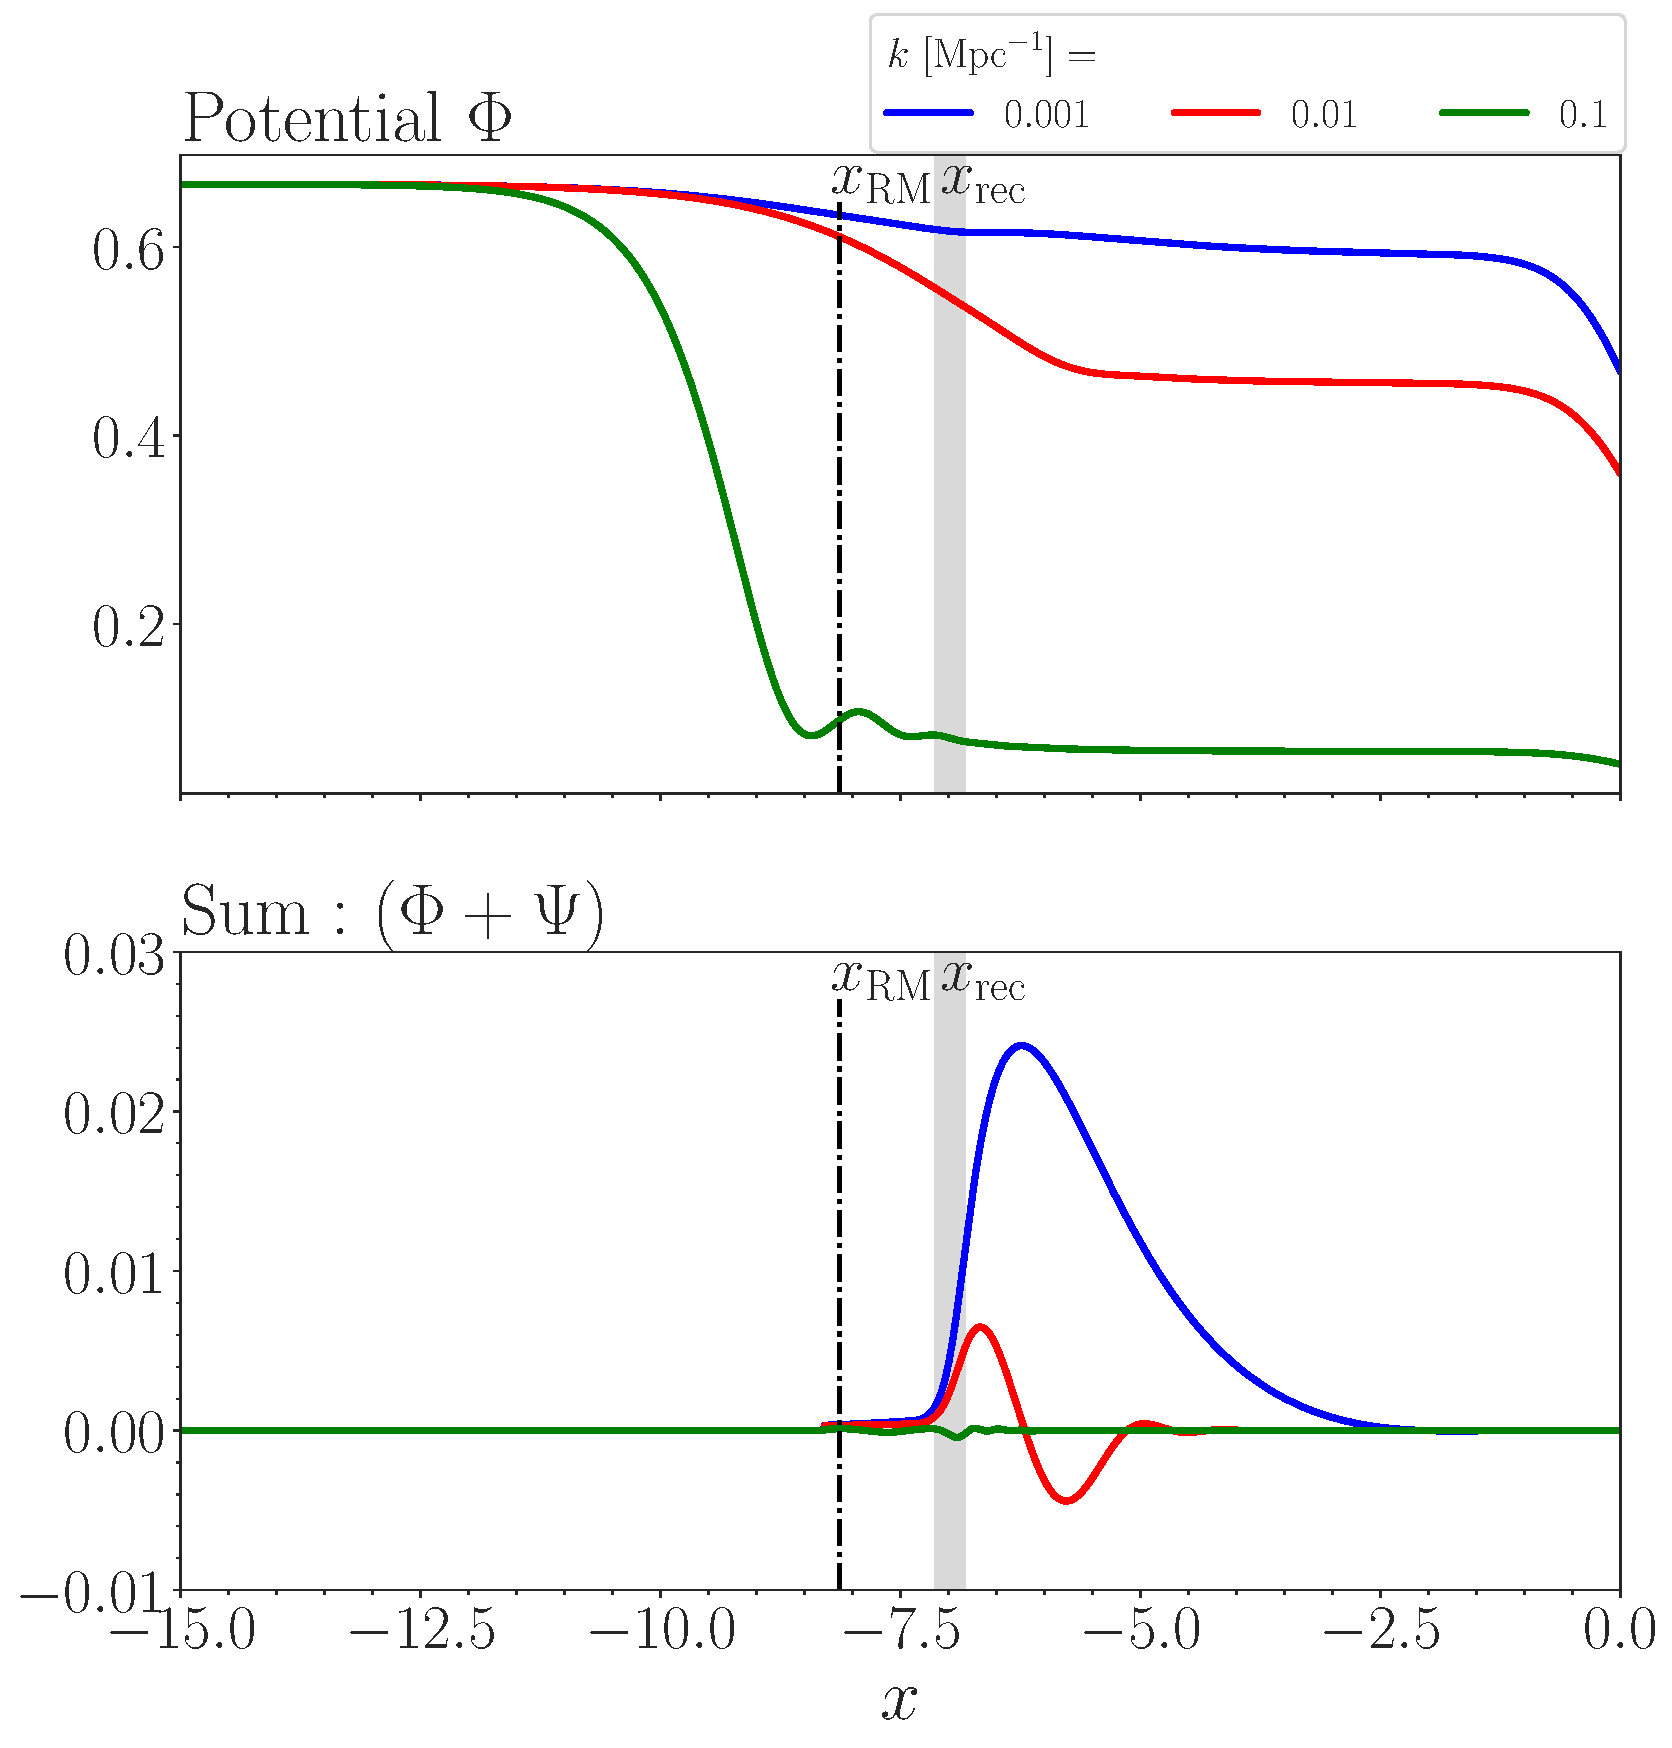
\includegraphics[width=\linewidth]{potentials.pdf}
        \caption{The metric perturbation potentials, $\Psi$ representing the Newtonian potential, and $\Phi$ representing the spatial curvature perturbation. Both panels show the evolution as function of the time $x$, for the three different $k$-modes outlined in ~\cref{sec:m3:methods}. The top panel shows $\Phi$ alone, while the bottom shows the sum of the two. The grey shaded are represent the time of recombinaiton as found in ~\cref{sec:m2}, highlighting the fact that it did not occur in an instant, and the dash-dotted black line is the time of radiation-matter equality as found in ~\cref{sec:m1}.}
        \label{fig:m3:potentials}
    \end{figure}

\subsubsection{Multipoles}
    We now focus our attention on the multipoles, starting with the monopole term expressed through the photon overdensity $\delta_\gamma = 4\T_0$. Mathematically, this relation can be seen  from either the parenthesis in ~\cref{eq:m3:theory:time_evolution_of_Phi} or the definition of $\mathcal{Y}$ in ~\cref{eq:m3:theory:metric_perturbations_final} following somewhat diffuse symmetry arguments. Physically it also makes sense since the photon monopole is some measure of the average photon temperature which intuitively can be though of as a photon overdensity. It can be seen for the various $k$-modes in ~\cref{fig:m3:monopole}, where we clearly see that the small scale perturbation undergoes horizon crossing first, and become subject to causal physics. This is manifest in the oscillation of the green curve in the figure. Metric perturbations and pressure will generate acoustic oscillations within causally connected regions. When the horizon increase, these oscillations will affect a spatially large area, affecting $k$-modes on larger and larger scales. This is also manifest in ~\cref{fig:m3:monopole} as the intermediate $k$-mode starts to oscillate later, and finally the large scale mode. 

    What are the monopole fluctuations really? The different modes represent the average temperature at different physical length scales. At early times, when the horizon is small, most modes are outside it, leaving their average temperature and thus monopole constant. As modes enter the horizon, they become subject to causal physics, like the gravitational potential. Since photons and baryons are coupled at early times, photons must continuously climb in and out of the gravitational potential wells set up by matter, gaining and loosing energy in the process. It is worth noticing that this manifest itself as oscillations in Fourier space, but can be interpreted as propagating acoustic waves in real space. Before recombination, for modes having entered the horizon, these are waves in the baryon-photon fluid, propagating with the speed of sound. The origin of these oscillations in the radiation era is the decay of the gravitational potentials (discussed in the previous section), an effect called \textit{radiation driving}. The oscillations are also asymmetric about its equilibrium position. This is due to \textit{baryon loading} where the potentials change slightly because of the oscillating baryons, whereas the radiation pressure is left unchanged. The fact that the baryons and photons move together affects the sound speed which also causes some asymmetry to the oscillations. After recombination, photons decouple from baryons and stream freely throughout the Universe. During this decoupling process the interaction rate between photons and baryons decreases, but does not become zero. There as still interactions, causing energy to be transported and, temperature fluctuations on small scales to become washed out. This is known as diffusion damping, and smooths out the small scale perturbation for both radiation and matter. This is manifest for the small scale mode in green in ~\cref{fig:m3:monopole} as its amplitude decays after recombination. This phenomenon is not present for the modes entering the horizon after decoupling, in the matter regime. 

    Thus, the photon monopole perturbation behaves somewhat according to ~\cref{eq:m3:theory:analytical_monopole_eom}, where the oscillations are sourced by some force term which is a function of the potentials. This is true before decoupling for modes having entered the horizon. Super-horizon modes hardly evolve at all, due to the lack of causal physics.
    \begin{figure}
        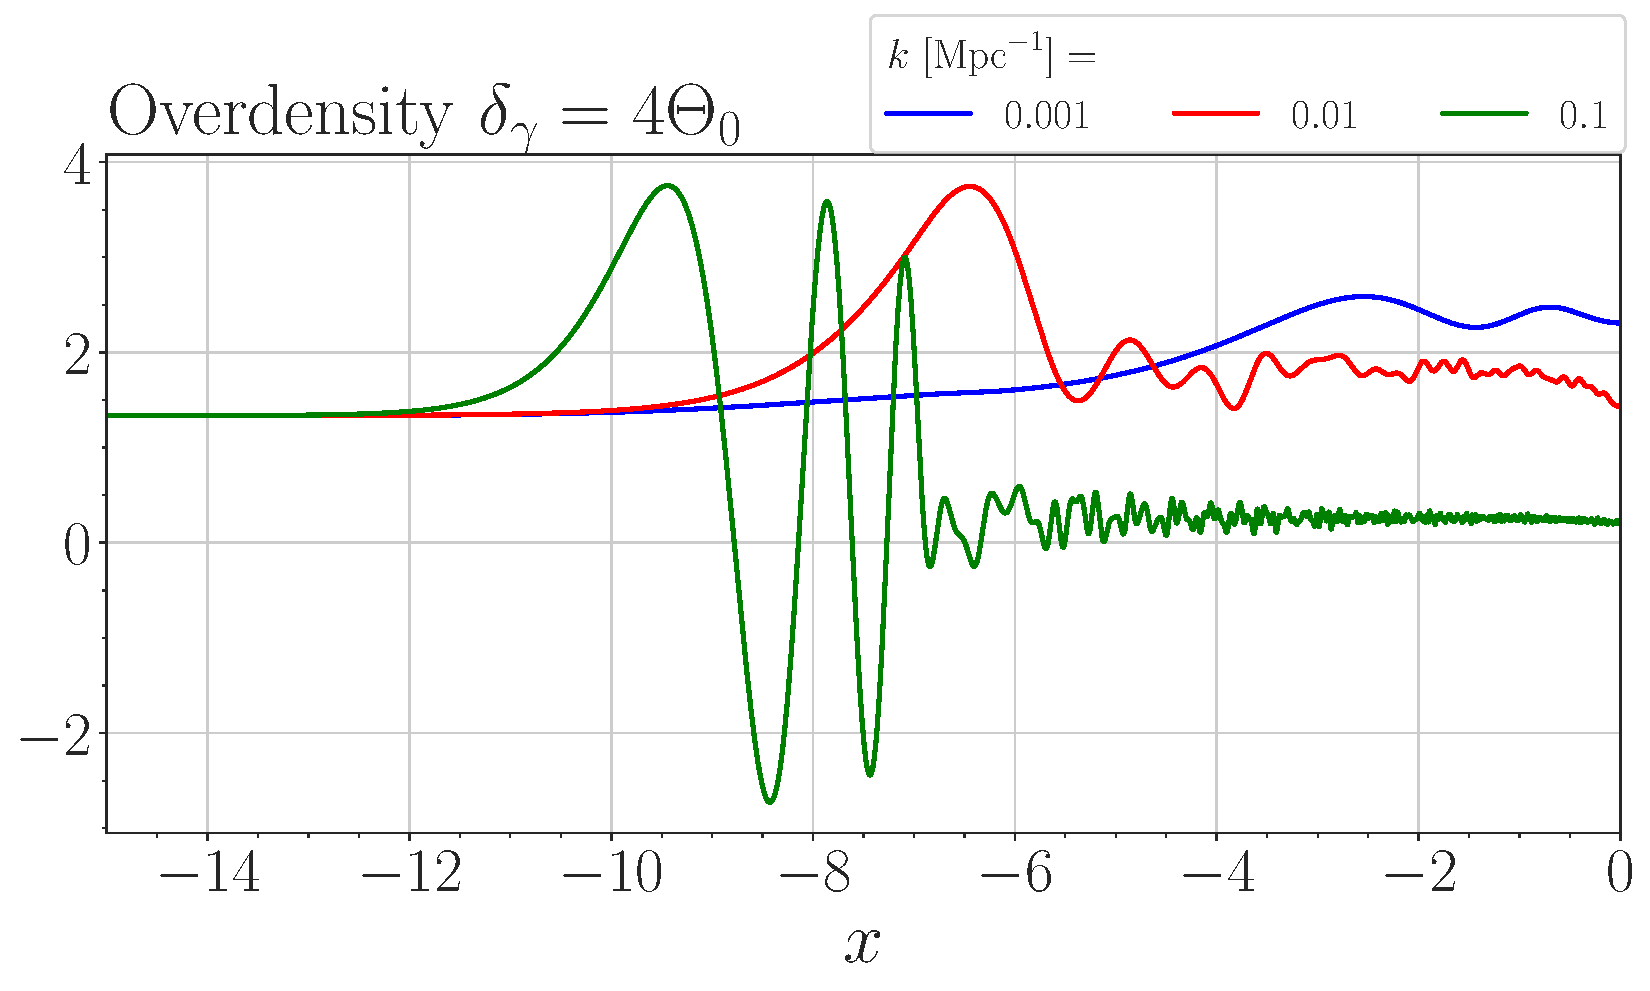
\includegraphics[width=\linewidth]{monopole.pdf}
        \caption{Photon overdensity represented by the photon monopole for the various $k$-modes. Recombination is marked as a shaded grey area. The time of radiation-matter equality is marked with a dashed black line.}
        \label{fig:m3:monopole}
    \end{figure}

    A similar discussion to the one above can be applied on the photon velocity $v_\gamma = -3\T_1$, as shown in ~\cref{fig:m3:dipole}. Similarly to the monopole, small scale modes enter the horizon first and starts to oscillate followed by larger scale modes. Modes entering the horizon before recombination experience diffusion damping, effectively smoothing the average velocity of the photons. Worth noticing in this plot is that for similar modes, the oscillatory behaviour of the photon velocity is starting slightly before the overdensity. This makes sense, since we need something to be moving in the first place for overdensities to occur. 

    \begin{figure}
        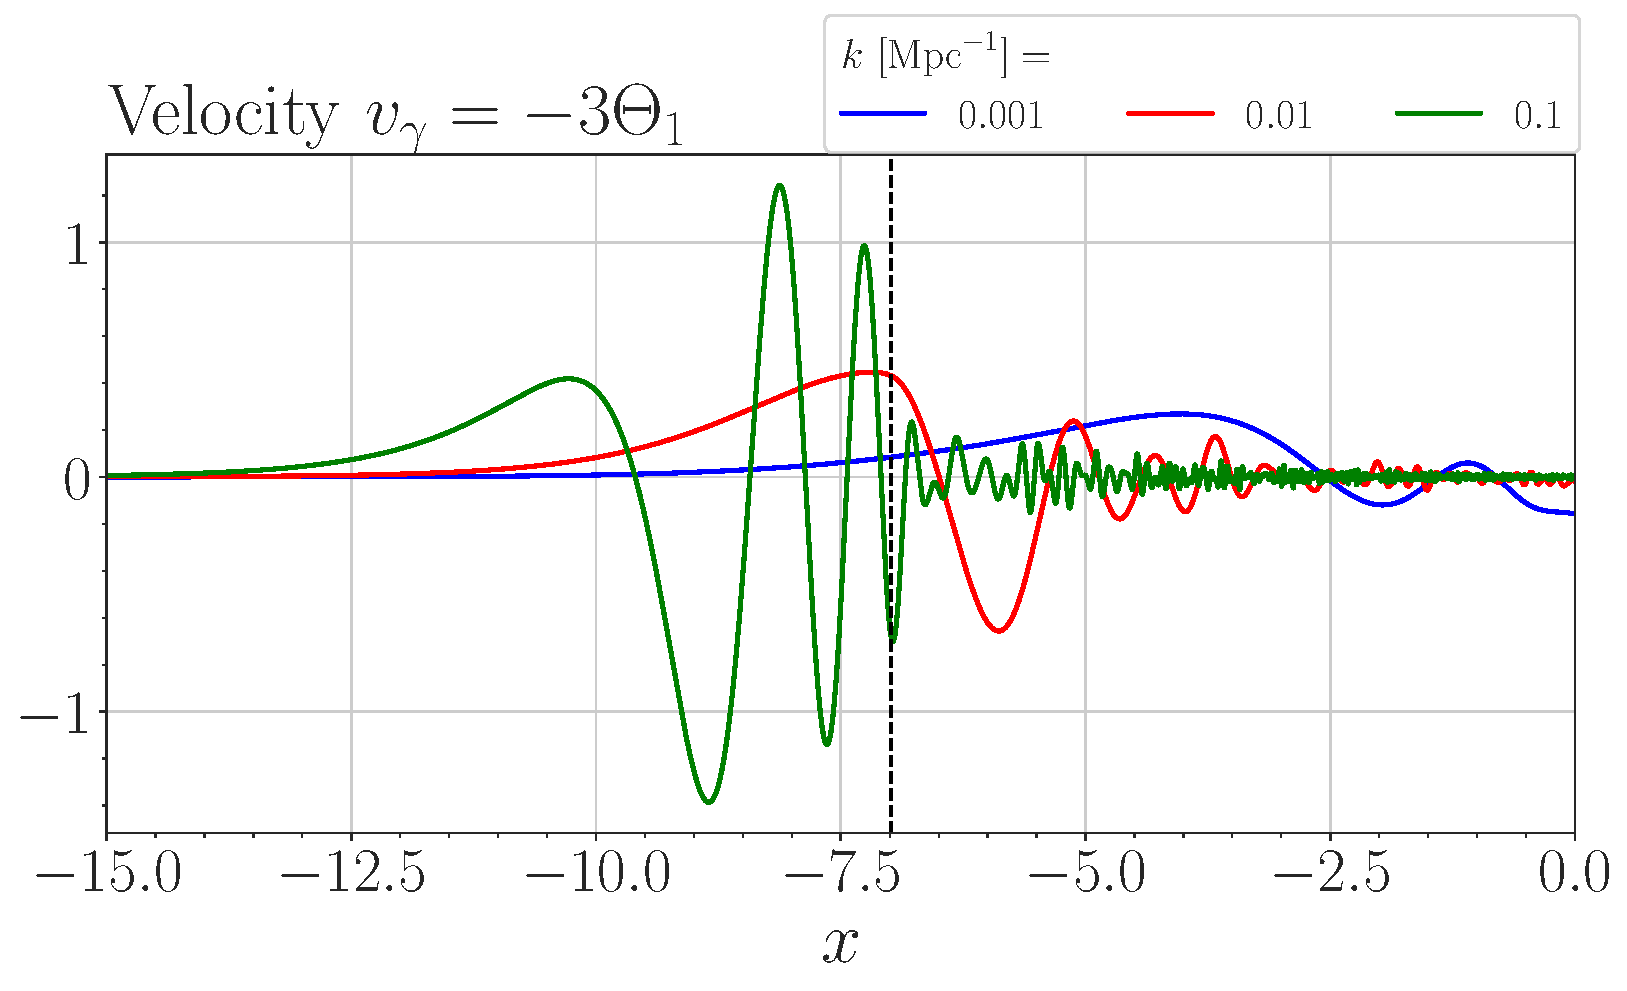
\includegraphics[width=\linewidth]{dipole.pdf}
        \caption{Photon velocity represented by the photon dipole for the various $k$-mdoes. Recombination is marked as a shaded grey area. The time of radiation-matter equality is marked with a dashed black line.}
        \label{fig:m3:dipole}
    \end{figure}

    The same is the case for the quadrupole in ~\cref{fig:m3:quadrapole}. However, as previously assumed, the quadrupole term is strongly suppressed during tight coupling, but behave similarly to the lower order multipoles after tight coupling. This is because during tight coupling, the photon-baryon plasma behaved very much like a fluid, only described by some average temperature and a velocity. Hence, there were no significant quadrupole (or any higher order multipole) moment(s) in this regime. Considering the large and intermediate scale modes (blue and red curve) we are able to close the discussion of the sum of potential in ~\cref{fig:m3:potentials}, where the quadrupole was the main contributor to the sinusoidal frequency, and $k$ to the amplitude. The small scales modes of the quadrupole experience the same diffusion damping as the lower multipoles. 

    \begin{figure}
        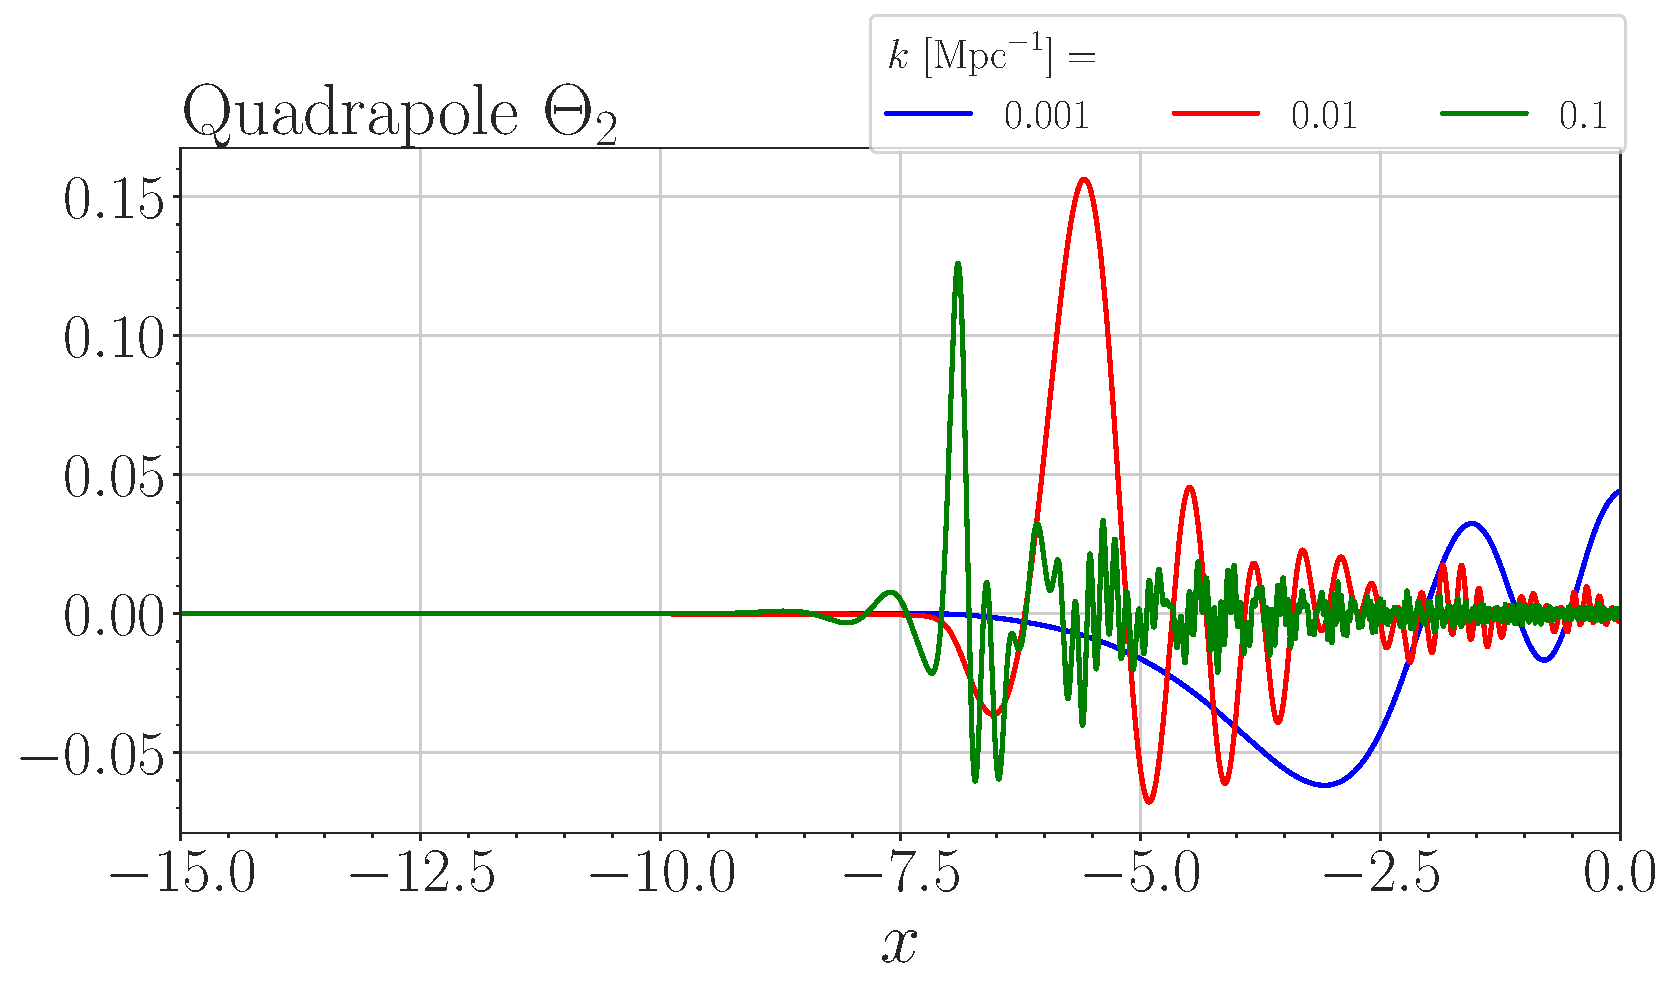
\includegraphics[width=\linewidth]{quadrapole.pdf}
        \caption{Quadrapole term of the photon perturbation. This term only becomes relevant after tight coupling. Recombination is marked as a shaded grey area. The time of radiation-matter equality is marked with a dashed black line.}
        \label{fig:m3:quadrapole}
    \end{figure}

\subsubsection{Matter perturbations}

    ~\cref{fig:m3:delta} show the overdensities of cold dark matter and baryons as function of time $x$, for the various $k$-modes. The small scale mode (green) enter the horizon during radiation domination, and immediately begins to cluster in overdense regions. The cold dark matter is not coupled to anything so its overdensity evolves on its own, only restricted by the growth of the Universe itself. During radiation domination, the rapid expansion of the universe makes the evolution of the cold dark matter logarithmic. Baryons, on the other hand, are coupled to photons and experiences photon radiation pressure which prevent their overdensities from growing. Instead, the interplay between radiation pressure and gravitation propagates acoustic sound waves in the plasma, manifest as oscillations in Fourier space. These are seen in the plot (green dashed line). These oscillations will continue as long as photons and baryons are coupled. As we transition from radiation to matter dominated, the evolution of the dark matter overdensity change from a logarithmic relationship to a power law scaling with the scale factor $a$. This is because the expansion rate of the Universe change alongside its dominant constituent, and when matter becomes dominant, the expansion rate decreases. This enables larger perturbations in the dark matter. The behaviour of the baryons change once they decouple from the photons. Now they do not feel the same radiation pressure as before, so they start to gather in the potential already in existence due to dark matter. This happens slightly after decoupling. There is a small delay due to compton drag, photons diffuse and scatter of baryons, and the baryons already have some velocity from the oscillation. \footnote{The width of the grey shaded area showing recombination cannot be taken literally as it is there just to showcase the fact that recombination and decoupling are not instantaneous processes.} From now on, the baryons fall into the gravitational wells, and all matter evolve together deep in matter domination. Close to $x=0$, when dark energy become the dominant constituent, the acceleration of the universe increases and the matter overdensities grow slower because of this.

    The intermediate scale mode enters the horizon around the time of radiation matter equality, so the baryons deviate slightly from the dark matter evolution. However, there is not any oscillatory behaviour since this mode did not enter the horizon early enough to capture the oscillations of the plasma. During matter dominating, all matter evolves similarly; growing as a power law w.r.t. the scale factor. The blue line representing large scale modes show this, entering the horizon deep in matter domination and immediately starts to grow according to this power law. 
    


    % For the matter perturbations, we start with the overdensities for cold dark matter and baryons, shown in ~\cref{fig:m3:delta}. Intuitively, we would expect small fluctuations in density to occur at very small scales early on, and then at larger scales gradually as the horizon increase. During the radiation dominated regime, expect the matter densities to be relatively homogenous on large scales, but noticeable on small scaler. In the matter dominated regime we expect overdense regions to attract more and more matter, increasing the overdensities. These effect should be noticeable on larger scales even, i.e. the modes that undergo horizon crossing during matter dominatin. When inspecting ~\cref{fig:m3:delta} this is indeed what we observe. The overdensity of the small scale mode in green starts to increase during radiation domination, large scale mode in blue during matter domination and the intermediate scale mode in red somewhere in between. All modes increase during matter domination which is what we expected. During dark energy domination we would expect the acceleration of the Universe to start to break up some structures and decrease the horizon, which would also decrease the matter overdensities. Lastly, we take note of the oscillations in the baryon density right before and after matter-radiation equality, but save the discussion for later. 

    \begin{figure}
        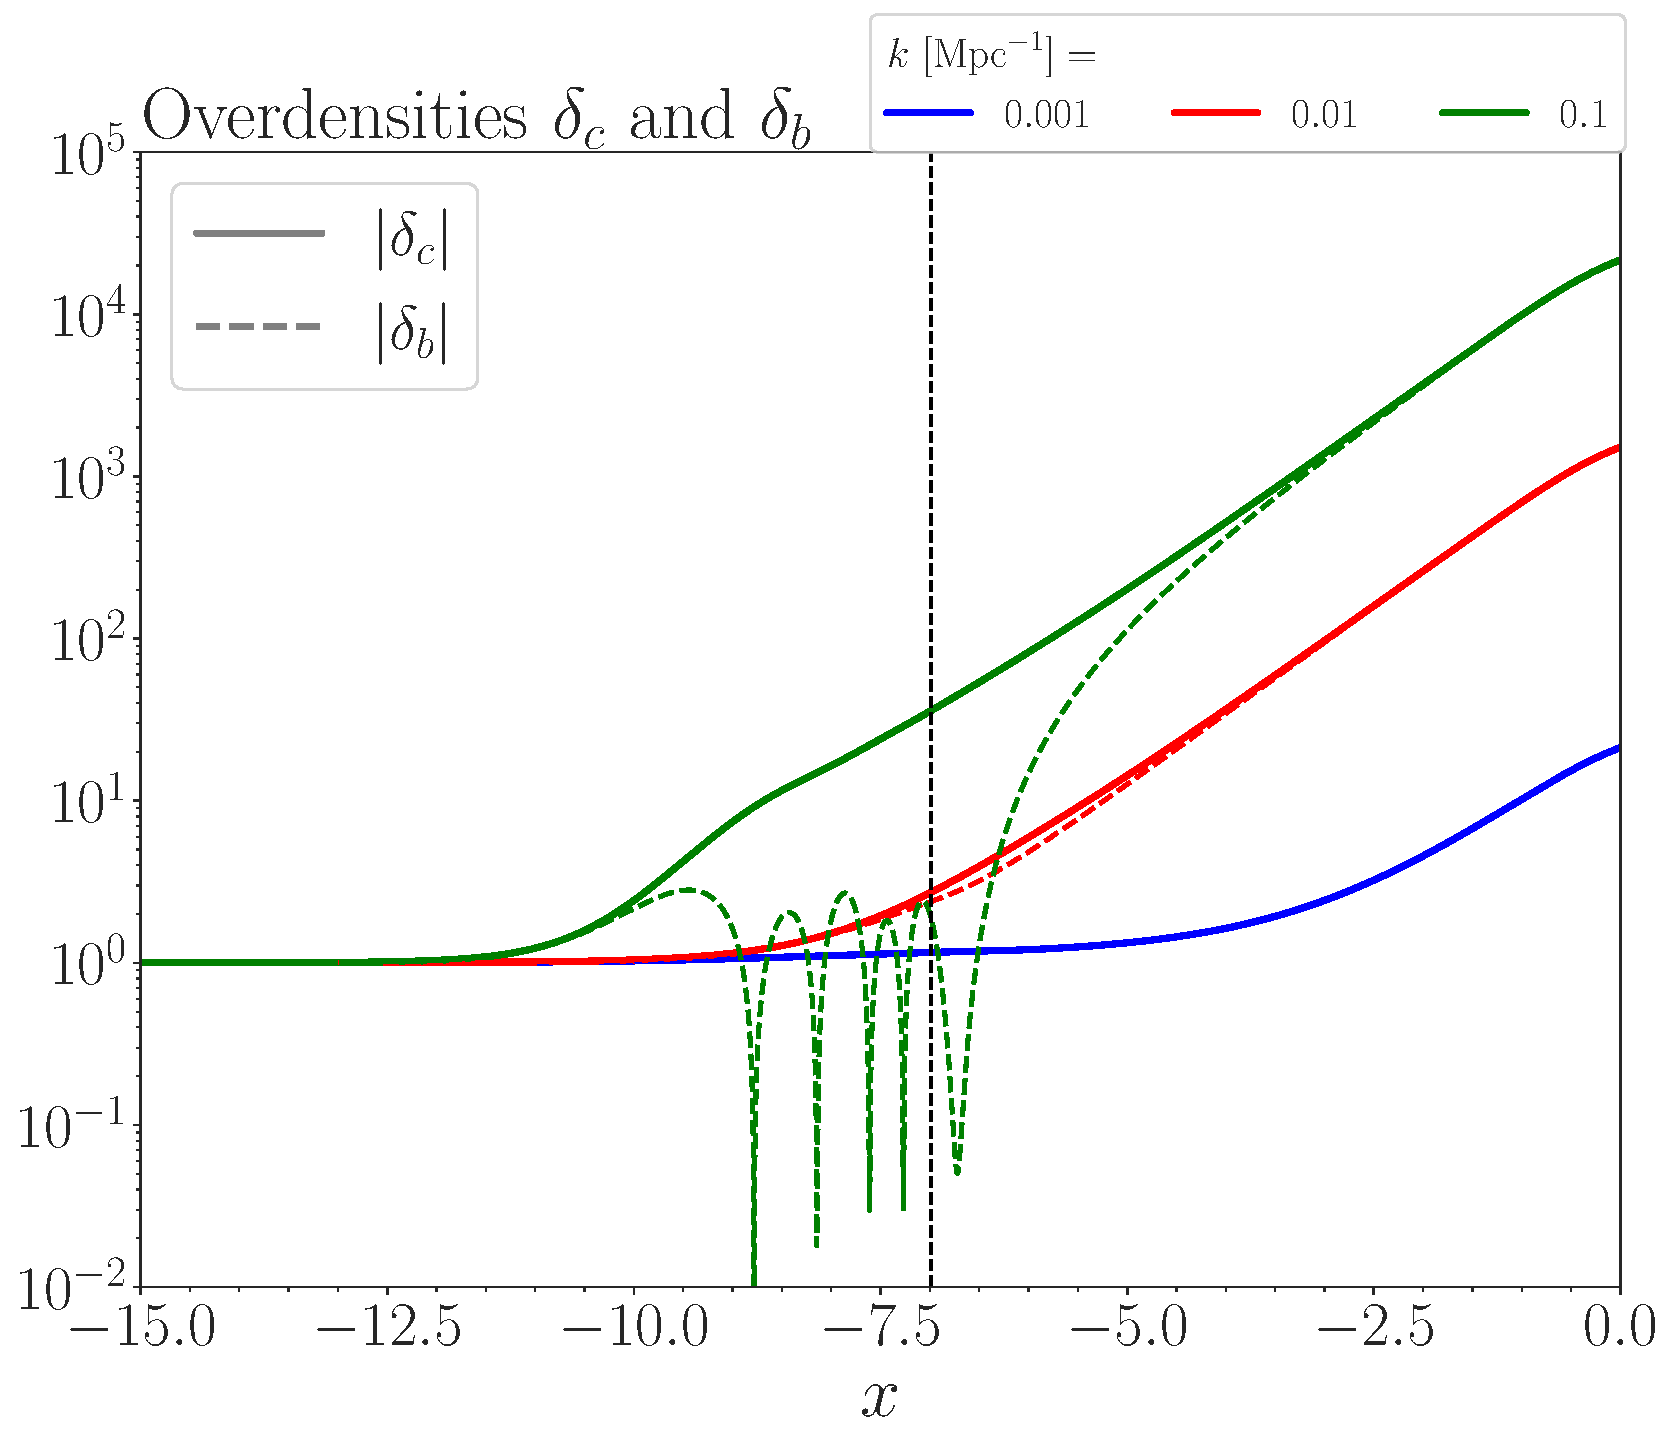
\includegraphics[width=\linewidth]{delta.pdf}
        \caption{The overdensities of cold dark matter and baryons for the various $k$-modes. Recombination is marked as a shaded grey area. The time of radiation-matter equality is marked with a dashed black line.}
        \label{fig:m3:delta}
    \end{figure}
    
    We emphasise the above discussion by considering only the small scale mode, and including the photon overdensity as well. This is shown in ~\cref{fig:m3:delta_comparison}. We recognise the dark matter and baryon overdensities, and we also clearly see the coupling between baryons and photons at early times, before recombination. After this, the baryon evolves as the dark matter, and the photons diffuse, reducing the amplitude of their oscillations, effectively smoothing their overdensitites. This diffusion drags out the time it takes for the baryons to fall in to the potentials (to keep up with dark matter). This is the effect of Compton drag, as diffusion is effectively photons interacting with electrons through Compton scattering, with an increased mean free path between each interaction. 

    \begin{figure}
        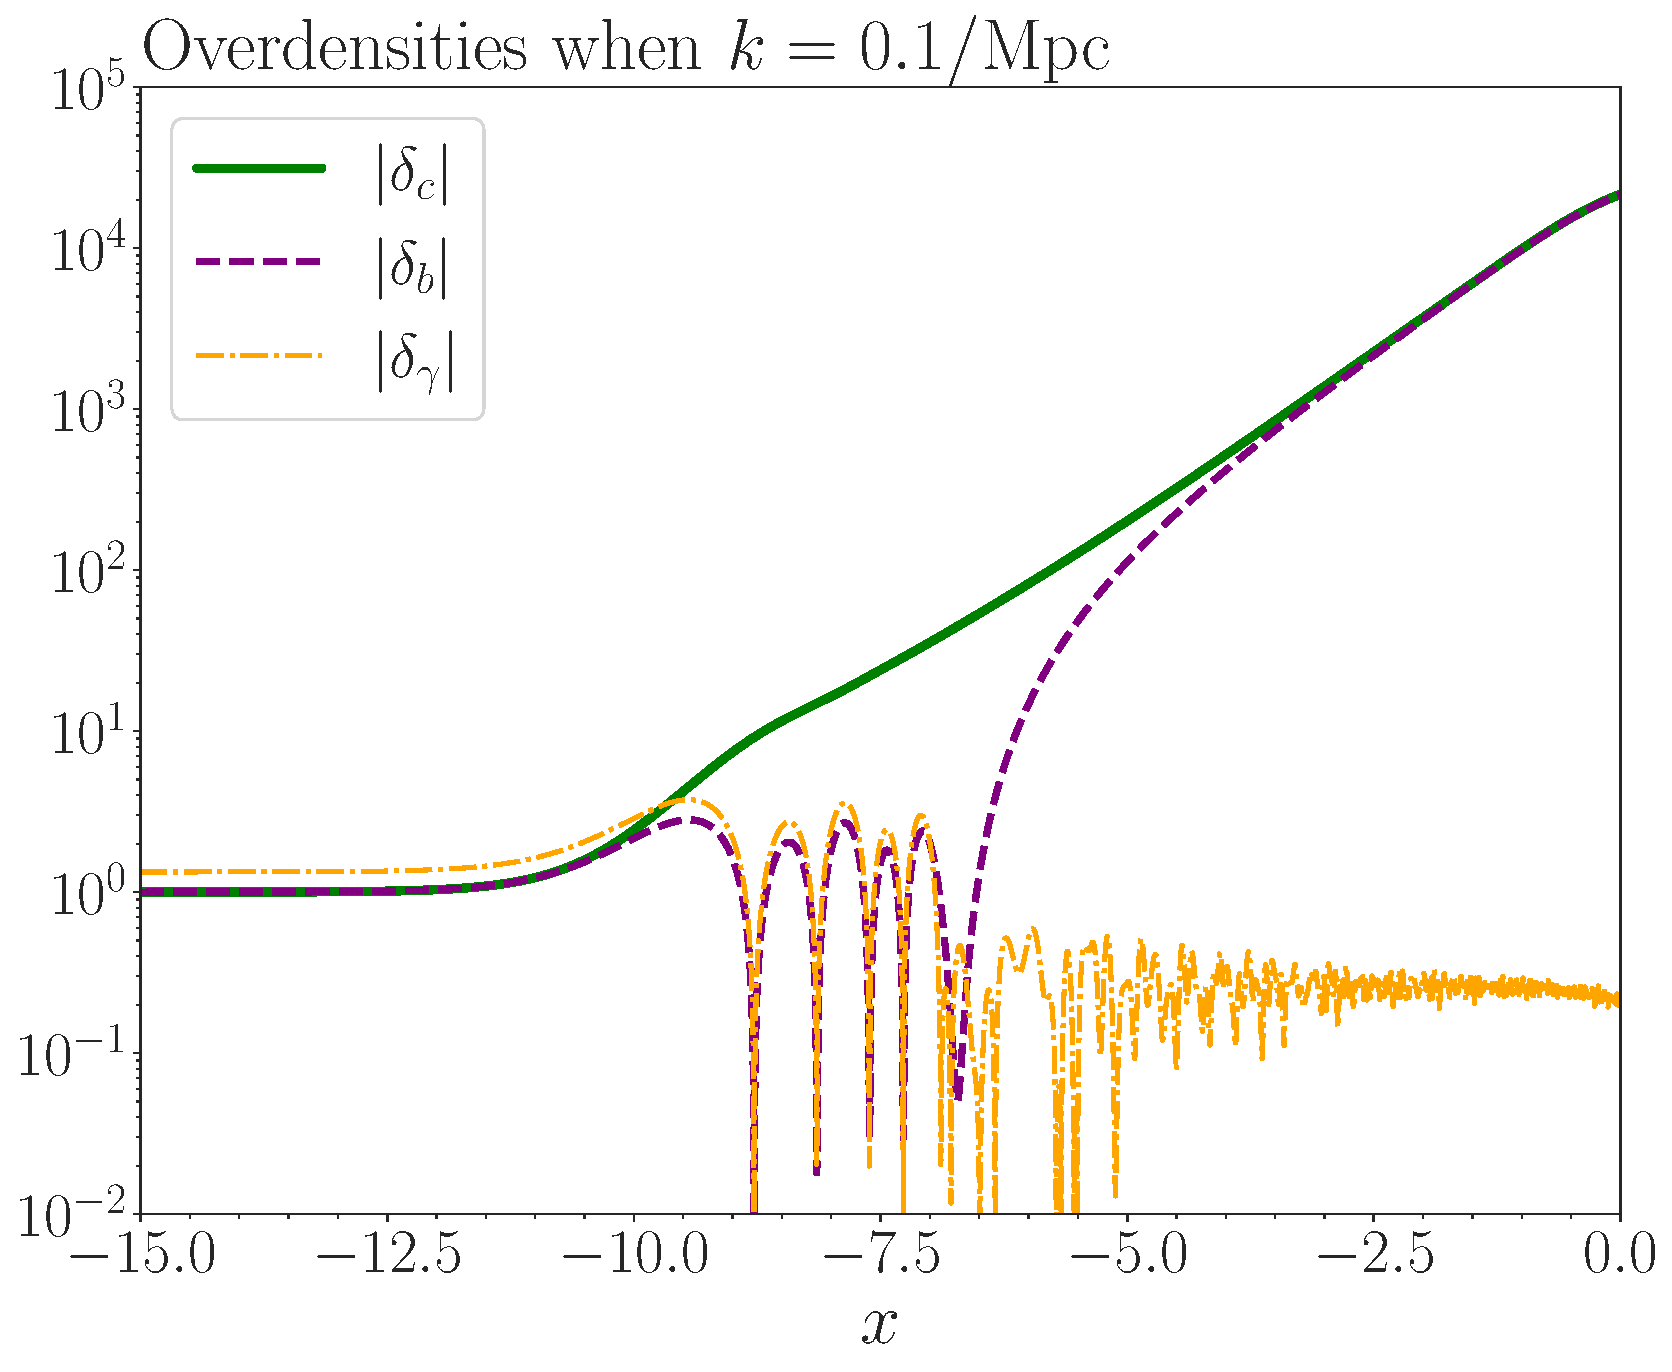
\includegraphics[width=\linewidth]{delta_comparison.pdf}
        \caption{Comparison of the overdensities of cold dark matter, baryons and photons for a small scale mode. We clearly see the decoupling of photons from baryons during recombination, which is marked as a shaded grey area. The time of radiation-matter equality is marked with a dashed black line. }
        \label{fig:m3:delta_comparison}
    \end{figure}
    
    
    % The remaining question to answer now is why does the baryon overdensity and velocity oscillate for the modes entering the horizon during radiation domination? In order to answer this question we consider the largest mode among the three; $k=0.1$/Mpc, and plot the velocities and overdensities of the cold dark matter, baryons and photons in the same plot. The result is seen in ~\cref{fig:m3:velocity_comparison} for the velocities and in ~\cref{fig:m3:delta_comparison} for the overdensities. We have already made statements about the oscillation of the photon velocity from ~\cref{fig:m3:dipole}, and photon overdensity from ~\cref{fig:m3:monopole}. The most important time in ~\cref{fig:m3:velocity_comparison} and ~\cref{fig:m3:delta_comparison} is the time of recombination (dashed line), which is closely related to the time of decoupling and last scattering, when the photons decouple from the baryons. Before this, baryons and photons are tightly coupled so we expect them to evolve similarly. It therefore makes sense that we have oscillations in the baryon velocity and overdensity before recombinations, as the baryons were tightly coupled to the photons. After decoupling, the baryon velocity and overdensity show similar behaviour to those of cold dark matter. At the same time, the oscillations of the photon monopole and dipole causes the photon velocity and overdensity to gradually decrease and converge as the photons free stream through the Universe. 

    ~\cref{fig:m3:velocity} show the velocities (bulk velocity of the fluid motion) of the cold dark matter and baryons. We start by noticing that for super-horizon scales (to the left of the plot), the velocities are the same for baryons and cold dark matter, and it follows the expansion of the Universe. It must be so, because no physics can affect the velocity which must be comoving as the Universe expands. For scales entering the horizon at late times it is always like this (blue line); the velocity follows the expansion of the Universe since the physical overdensity is in the same comoving location (for large scales). For baryons entering the horizon during radiation domination (small scales) it is a different story as this is an acoustic wave travelling outwards with some velocity. This is captured as oscillations in ~\cref{fig:m3:velocity}. The cold dark matter overdensities for small scales will also have a bulk velocity relative to the comoving coordinate system as these overdensities are subjected to the changing potentials. ~\cref{fig:m3:velocity_comparison} compares the bulk velocities of cold dark matter, baryons and photons for a small scale mode. Once again we notice the decoupling of the photons after recombinations. This plots tells pretty much a similar story as ~\cref{fig:m3:delta_comparison}.

    \begin{figure}
        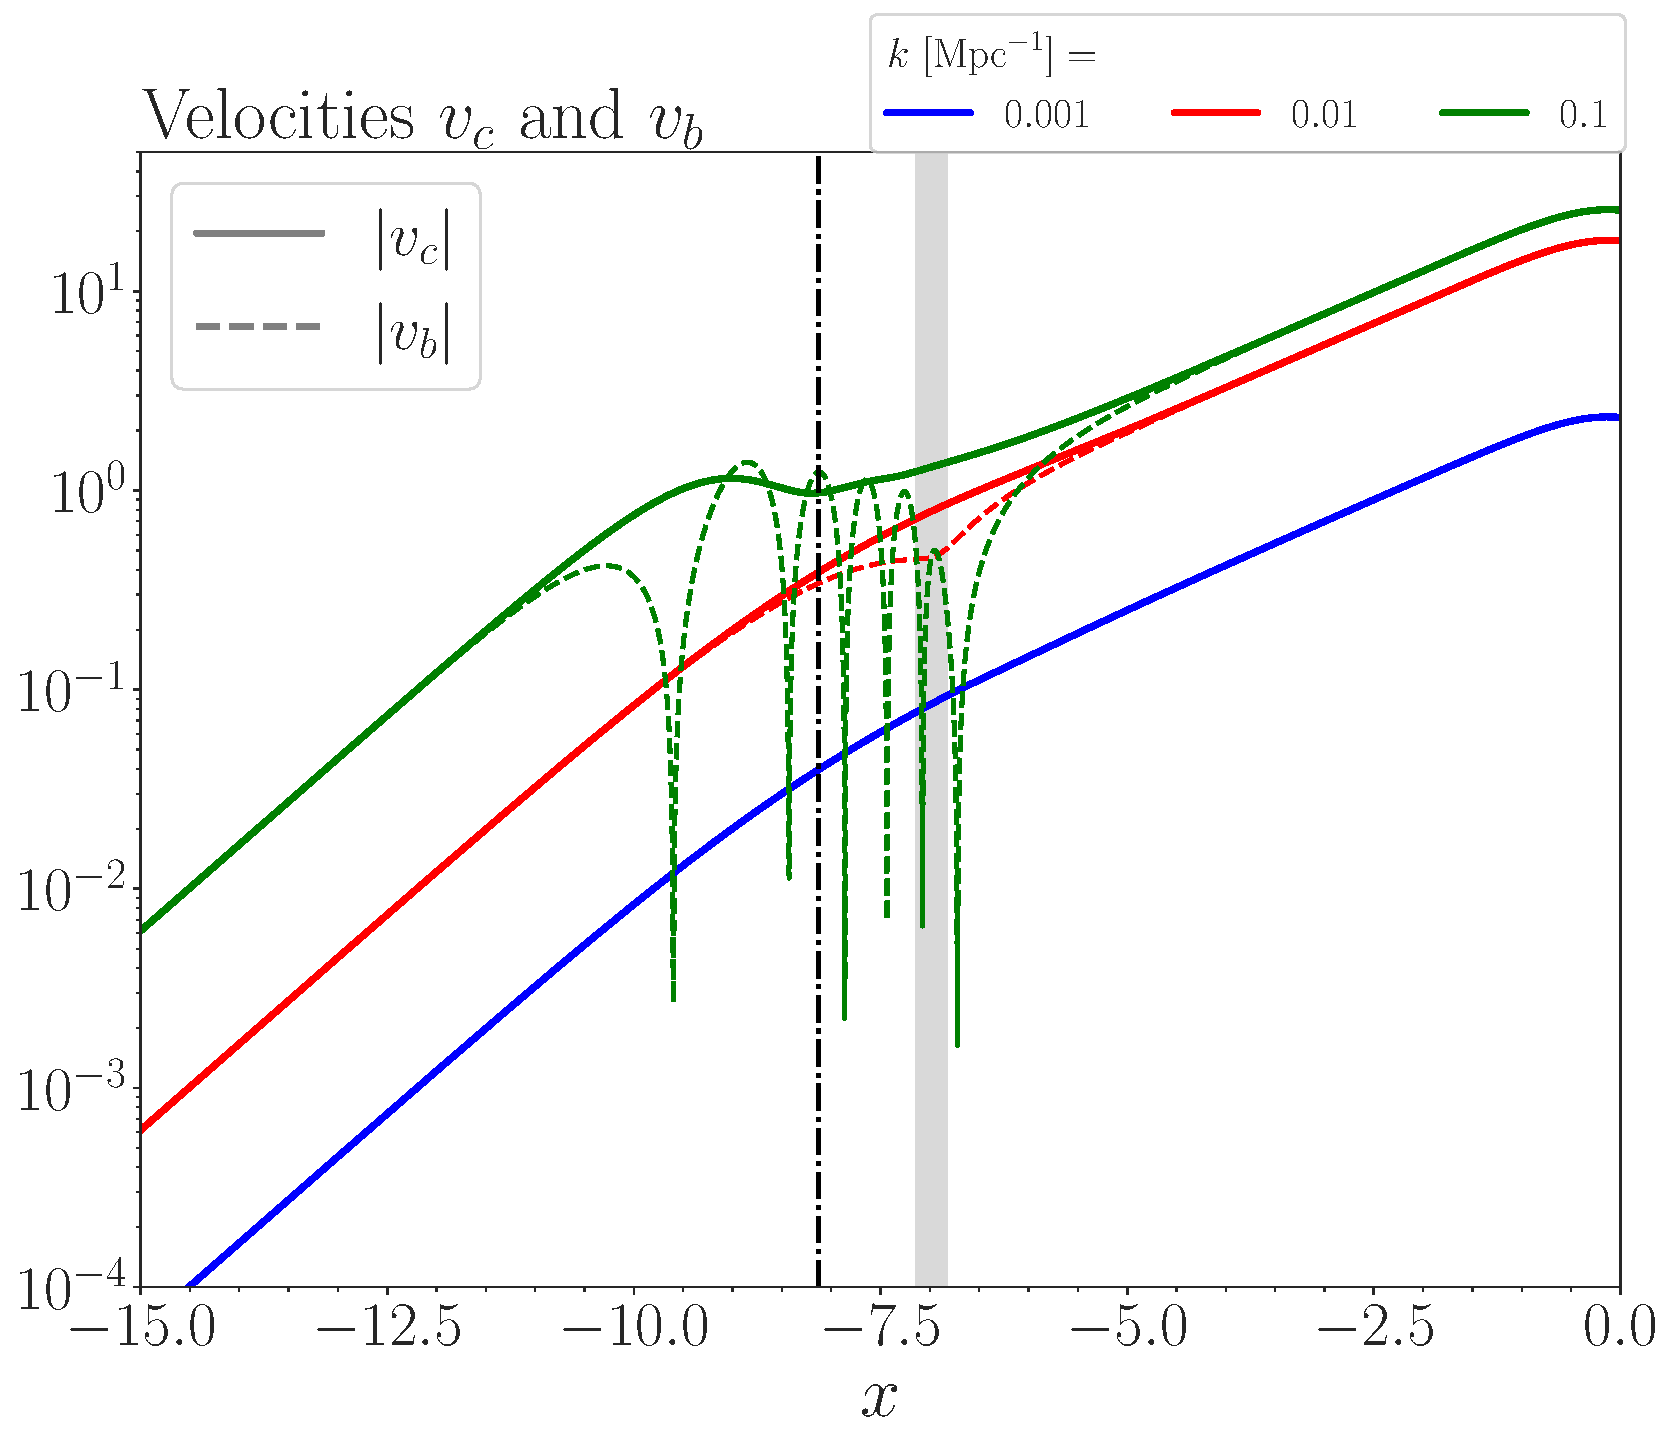
\includegraphics[width=\linewidth]{velocity.pdf}
        \caption{The bulk velocities of cold dark matter and baryons for the various $k$-modes. Recombination is marked as a shaded grey area. The time of radiation-matter equality is marked with a dashed black line.}
        \label{fig:m3:velocity}
    \end{figure}
    
    \begin{figure}
        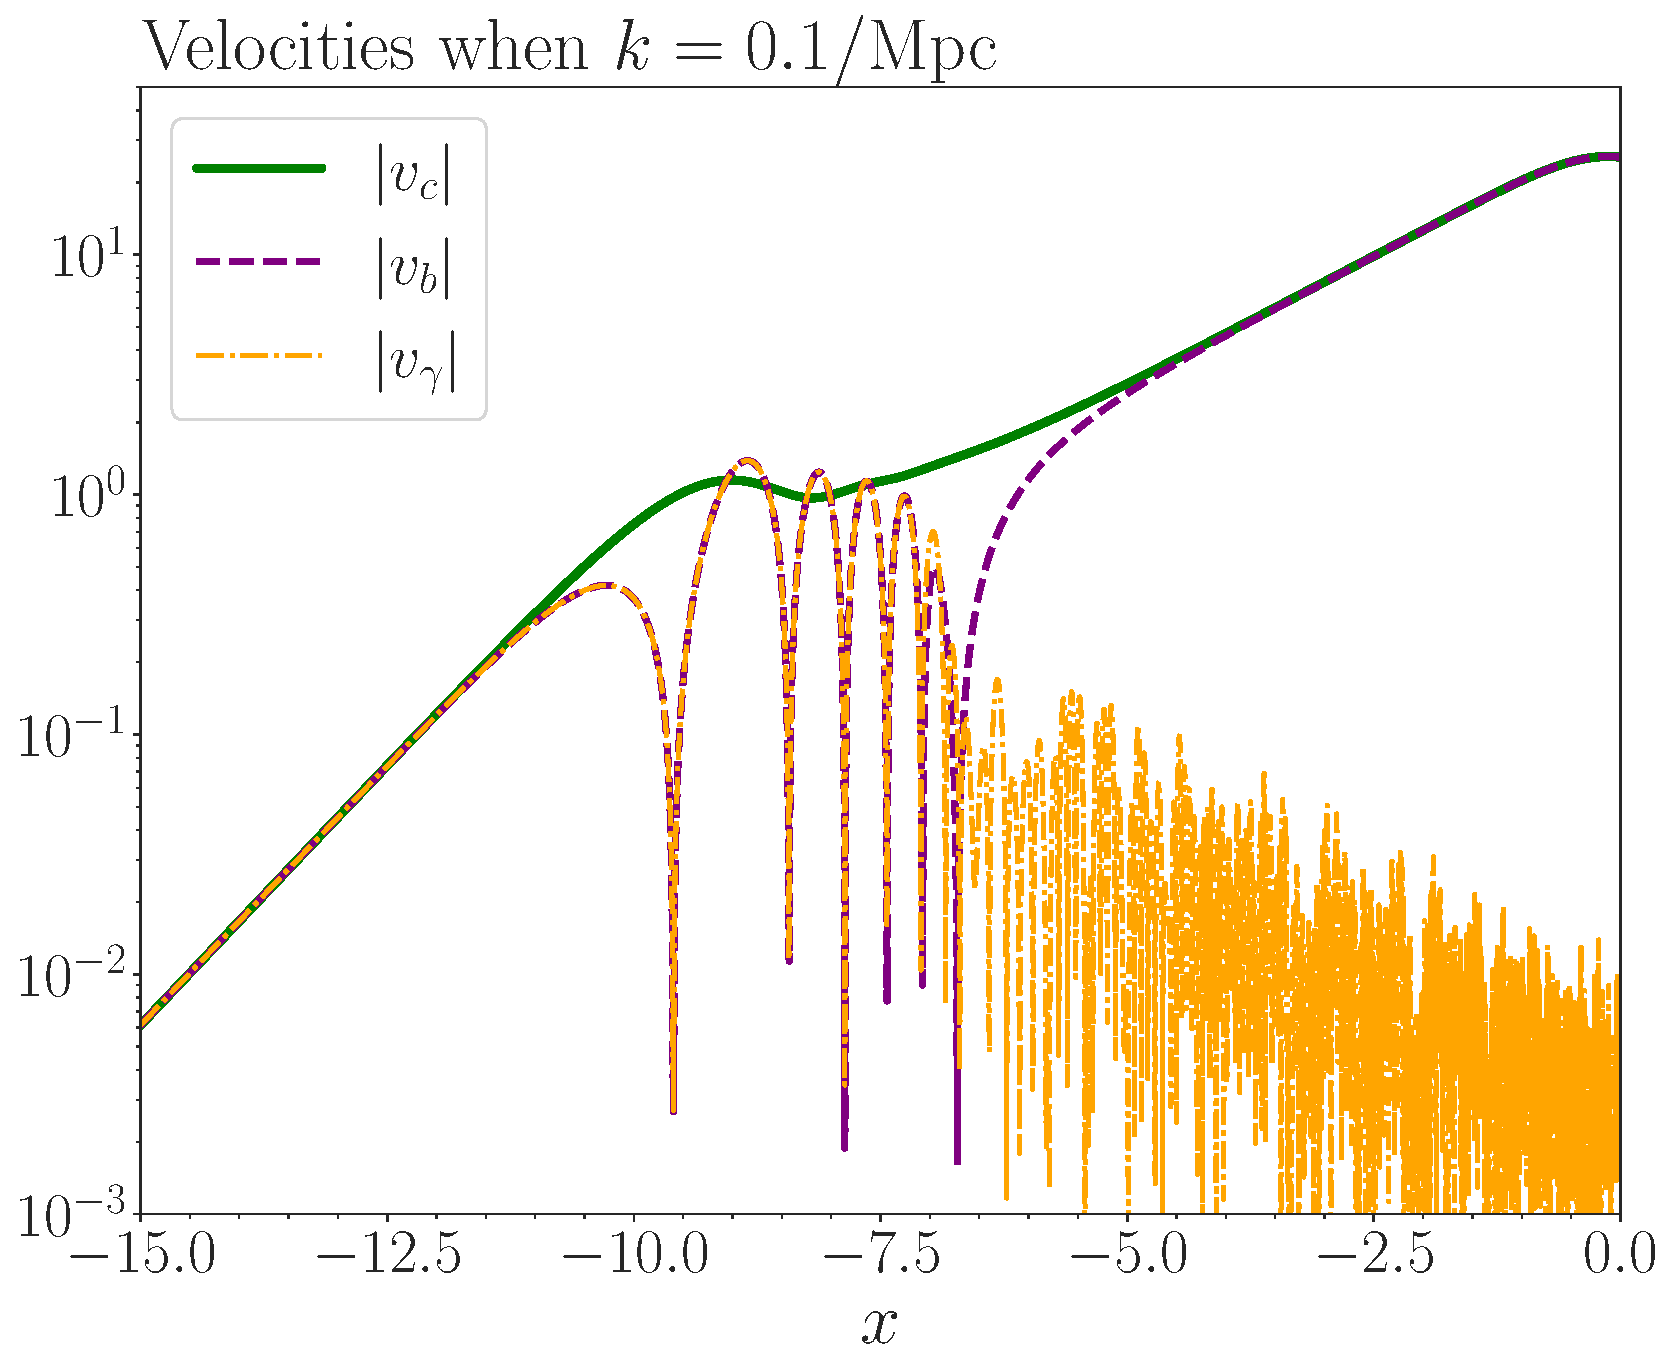
\includegraphics[width=\linewidth]{velocity_comparison.pdf}
        \caption{Comparison of the bulk velocities of cold dark matter, baryons and photons for a small scale mode. We clearly see the decoupling of photons from baryons during recombination, which is marked as a shaded grey area. The time of radiation-matter equality is marked with a dashed black line.}
        \label{fig:m3:velocity_comparison}
    \end{figure}
    


\section{Power spectrums}\label{sec:m4}

In this section we will construct the angular power spectrum and the matter power spectrum in order to compare our theoretical predictions with actual observables.

\subsection{Theory}\label{sec:m4:theory}
    Before delving into the theory of power spectrum we must make one distinction clear: When we studied the evolution of the temperature perturbation $\T$ in ~\cref{sec:m3:theory} we divided the evolution into two stages, namely the initial value of the perturbation, set up by inflation, and the evolution in time. We are able to treat them separately since we only consider perturbations to first order. We had that the initial perturbations were caused by the curvature perturbation $\mathcal{R}$. The evolution from initial perturbations to observable anisotropies is called the \textit{transfer function} and is the quantity, $\T$, for which we have already developed equations of motion, and will be solved for in our code. When solving we simply put $\mathcal{R}=1$,\footnote{This works as a normalisation, and can only be factored out if we work with linear perturbation theory. For any higher order, the initial perturbations must be including before evolving the system in time.} but if we want to compare our results to actual observables we need to include the initial perturbations. Thus:
    \begin{equation}
        \To_l(\vec{k},t) = \T_l(k,t)\mathcal{R}(\vec{k}) \iff \T_l(k,t)=\frac{\To_l(\vec{k},t)}{\mathcal{R}(\vec{k})}.
    \end{equation}
    $\T$ is referred to as $\mathcal{T}$ (transfer function) in ~\cite{dodelson2020modern}.
    \subsubsection{Physical observables}
        In order to measure the CMB we measure the temperature fluctuations as function of direction on the sky. In order to connect theory to these observations, we consider the temperature perturbation from ~\cref{eq:m3:theory:temperature_perturbation}, which is what we measure in experiments, and realise that this may be expanded in spherical harmonics (now in real space):
        \begin{equation}\label{eq:m4:theory:spherical_harmonic_expansion}
            \To(\vec{x}, \hat{\vec{p}}, t) = \sum_{l=1}^\infty\sum_{m=-l}^l a_{lm}(\vec{x}, t)Y_{lm}(\hat{\vec{p}}),
        \end{equation}
        where the angular dependency is taken care of by the \textit{spherical harmonic functions}: $Y_{lm}(\hat{\vec{p}})$. From orthogonality of spherical harmonics,\footnote{Orthogonality of spherical harmonics:$$\int\d\O_{\hat{\vec{p}}}Y_{lm}(\hat{\vec{p}})Y^*_{l'm'}(\hat{\vec{p}}) = \delta_{ll'}\delta_{mm'}$$} we may express the coefficient $a_{lm}(\vec{x},t)$ as:
        \begin{equation}\label{eq:m4:theory:alm_coefficients}
            a_{lm}(\vec{x},t) = \int\d\O_{\hat{\vec{p}}}Y^*_{lm}(\hat{\vec{p}})\To(\vec{x}, \hat{\vec{p}},t).
        \end{equation}
        It is important to note that ~\cref{eq:m4:theory:spherical_harmonic_expansion} allows us to divide the temperature perturbations into a set of weighted basis functions, these being the spherical harmonics. These functions are eigenfunctions of the Laplace operator on a sphere, and describe how a function varies with direction (on a sphere). The $l$-subscript indicates the scale on which these variations occur (these are inversely proportional). Thus, the interpretation of the $a_{lm}$ coefficient is the amplitude of temperature fluctuations across different scales, $l$. Since inflation predicts initial perturbations like $\T$ to be Gaussian random fields it follows that the $a_{lm}$-s are also Gaussian random fields with mean 0 and variance $C_l$ which is given by: 
        \begin{equation}\label{eq:m4:theory:alm_coeff_variance}
            \langle a_{lm}a^*_{l'm'}\rangle = \delta_{ll'}\delta_{mm'}C_l.
        \end{equation}
        Because of the Gaussian nature of $C_l$, it contains all the statistical information about $\T$, and this is what we refer to as the \textit{angular power spectrum} (or just power spectrum). Thus, when making observations of the CMB, the $a_{lm}$-s are measured and the corresponding power spectrum is constructed as ~\cite{AST5220LectureNotes}:
        \begin{equation}\label{eq:m4:theory:C_l_estimate}
            \hat{C}_l = \frac{1}{2l+1}\sum_{m=-l}^l\abs{a_{lm}}^2,
        \end{equation}
        where $\hat{C}_l$ is an estimator of the full power spectrum $C_l$, based on one realisation of the initial Gaussian random field, namely the realisation that is our observable Universe. For each $l$, we have $2l+1$ $m$ values from which we infer the estimate in ~\cref{eq:m4:theory:C_l_estimate}. Since we only have one universe to make measurements in, the statistical uncertainties of $\hat{C}_l$ is highly dependent on $l$, since for low $l$ there are very few components to measure. This gives rise to an intrinsic uncertainty in $C_l$ known as \textit{cosmic variance} which is governed by ~\cite{dodelson2020modern}:
        \begin{equation}\label{eq:m4:theory:cosmic_variance}
            \left(\frac{\Delta C_l}{C_l}\right) = \sqrt{\frac{2}{2l+1}}
        \end{equation}

    \subsubsection{Constructing the angular power spectrum}
        When constructing an equation for $C_l$ we start from ~\cref{eq:m4:theory:alm_coefficients} and expand this in it Fourier series:
        \begin{equation}\label{eq:m4:theory:alm_fourier}
            a_{lm} = \int\d\O_\hv{p}Y_{lm}^*(\hv{p})\int\frac{\d^3\vec{k}}{\pifac}e^{i\vec{k}\cdot{\vec{x}}}\To(\vec{k}, \hv{p},t),
        \end{equation}
        which we further expand into multipoles
        \begin{equation}\label{eq:m4:theory:alm_multipole_expansion}
            a_{lm} = \int\d\O_\hv{p}Y_{lm}^*(\hv{p})\int\frac{\d^3\vec{k}}{\pifac}e^{i\vec{k}\cdot{\vec{x}}} \sum_{l=1}^\infty(2l+1)(-i)^l\mathcal{P}_l(\mu)\To_l(\kv,t),
        \end{equation}
        where $\mu=\hv{p}\cdot\hv{k}$. Next, we multiply with the complex conjugate $a_{lm}^*$ in order to obtain:
        \begin{equation}\label{eq:m4:theory:almalm*}
            \begin{split}
                a_{l_1m_1}a_{l_2m_2}^* &= \sum_{l_1=1}^\infty\sum_{l_2=1}^\infty(2l_1+1)(2l_2+1)(-i)^{l_1-l_2} \\
                &\cross\int\frac{\d^3\kv_1}{\pifac}\int\frac{\d^3\kv_2}{\pifac}e^{i(k_1-k_2)}\\
                &\cross\int\d\O_{\hv{p}_1}\mathcal{P}_{l_1}(\mu_1)Y_{l_1m_1}^*(\hv{p}_1)\To_{l_1}(\kv,t) \\
                &\cross\int\d\O_{\hv{p}_2}\mathcal{P}_{l_2}(\mu_2)Y_{l_2m_2}(\hv{p}_2)\To_{l_2}(\kv,t),
            \end{split}
        \end{equation}
        which is a rather undelicate expression. Thankfully, there are a number of ways to make this simpler. Firstly, we note that 
        \begin{equation}\label{eq:m4:theory:alm_averaging_dependency}
            \begin{split}
                \langle a_{l_1m_1}a_{l_2m_2}^*\rangle &\sim \langle\To_{l_1}(\kv_1,t)\To_{l_2}(\kv_2,t)\rangle \\
                &= \T_{l_1}(k_1,t)\T_{l_2}(k_2,t)\langle\mathcal{R}(\kv_1)\mathcal{R}(\kv_2)\rangle,
            \end{split}
        \end{equation}
        where it follows from our Fourier normalisation convention that $\langle\mathcal{R}(\kv_1)\mathcal{R}(\kv_2)\rangle = \delta^{(3)}(\kv_1-\kv_2)P_\mathrm{prim}(k)$, where $P_\mathrm{prim}(k)$ is the \textit{primordial power spectrum}. This delta function will simplify the $k$-integrals by demanding $\kv=\kv_1=\kv_2$. 

        Further, there is a very useful identity of spherical harmonics, which read ~\cite{dodelson2020modern}:
        \begin{equation}\label{eq:m4:theory:spherical_harmonic_identity}
            \int\d\O_\hv{p}Y^*_{l_2m_1}(\hv{p})\mathcal{P}_{l_1}(\mu_1) = \delta_{l_1l_2}\frac{4\pi}{2l_1+1}Y_{l_1m_1}^*(\hv{k}).
        \end{equation}
        From ~\cref{eq:m4:theory:spherical_harmonic_identity} we pick up a factor $\delta_{ll_1}\delta_{ll_2}$, which will remove the two infinite sums in ~\cref{eq:m4:theory:almalm*}. We also rewrite the differential $\d^3\kv = k^2\d k\d\O_\hv{k}$. Ultimately, averaging over all ensembles of ~\cref{eq:m4:theory:almalm*} yield:
        \begin{equation}\label{eq:m4:theory:getting_to_the C_l}
            \begin{split}
                \langle a_{l_1m_1}a_{l_2m_2}^*\rangle &= \frac{(4\pi)^2}{(2\pi)^3}\delta_{l_1l_2}\int k^2\d k\T_{l_1}(k,t)\T_{l_2}(k,t) \\
                &\cross \int\d\O_\hv{k}Y_{l_1m_1}^*(\hv{k})Y_{l_2m_2}(\hv{k})\cross P_\mathrm{prim}(k)\\
                &= \frac{2}{\pi}\int k^2\d k\abs{\T_l(k,t)}^2P_\mathrm{prim}(k)\delta_{l_1l_2}\delta_{m_1m_2},
            \end{split}
        \end{equation}
        where we used orthogonality of the spherical harmonic in the last step. Comparing this to ~\cref{eq:m4:theory:alm_coeff_variance} yield the desired equation for the angular power spectrum:
        \begin{equation}\label{eq:m4:theory:Cl_integral_intermediate}
            C_l = \frac{2}{\pi}\int k^2 P_\mathrm{prim}(k)\abs{\T_l(k)}^2\d k,
        \end{equation}
        where we have made it implicit that we evaluate today: $\T_l(k) = \T_l(k,t_0)$. In order to simply this even more we take into account that most inflationary models predict the primordial power spectrum to be of the form ~\cite{dodelson2020modern}: \footnote{In the special case that $n_s=1$, the primordial power spectrum is called a \textit{Harrison-Zel'dovich} power spectrum.}
        \begin{equation}\label{eq:m4:theory:primordial_power_spectrum}
            P_\mathrm{prim}(k) = \frac{2\pi^2}{k^3}A_s\left(\frac{k}{k_\mathrm{pivot}}\right)^{n_s-1},
        \end{equation}
        which is characterised by its amplitude $A_s$ and spectral index $n_s$. Armed with this, the power spectrum then becomes:
        \begin{equation}\label{eq:m4:theory:power_spectrum_logk}
            C_l = 4\pi\int_0^\infty A_s\left(\frac{k}{k_\mathrm{pivot}}\right)^{n_s-1}\abs{\T_l}^2\frac{\d k}{k},
        \end{equation}
        where we now integrate across the logarithm of $k$. It is worth noting that the quantity found theoretically from ~\cref{eq:m4:theory:power_spectrum_logk} is fundamentally different from the power spectrum we measure and construct using ~\cref{eq:m4:theory:C_l_estimate}. This is because when evaluating ~\cref{eq:m4:theory:getting_to_the C_l} we average across the whole ensemble of possible realisations of the primordial Gaussian random field. Thus, the quantity we arrive at theoretically is the \textit{ensemble averaged power spectrum}, while we are only able to observe the power spectrum for the one realisation that is our universe. However, when observing for large $l$-s we average across a large number of modes, which according to the \textit{ergothic assumption} will be the same as the ensemble average ~\cite{AST5220LectureNotes}. Thus, we are able to accurately estimate $C_l$ for sufficiently large $l$-s, but should run into cosmic variance for small $l$-s. 

        On last point to consider is that for a scale-invariant spectrum ($n_s=1$), the contributions from the Sachs-Wolfe terms yields ~\cite[Eq. 9.80]{dodelson2020modern}:
        \begin{equation}
            l(l+1)C_l^\mathrm{SW} = \frac{8}{25} A_s,
        \end{equation}
        which is constants. Thus, it is conventional to consider the quantity $\sim l(l+1)C_l$ and consider any deviations away from a constant horisontal line. 

    \subsubsection{Matter power spectrum}
        The matter power spectrum described the distribution of fluctuations in the matter density field in terms of scale. Evaluating it today yield information about the matter density at different physical scales, as we observe it today. It is given as ~\cite{AST5220LectureNotes}:
        \begin{equation}\label{eq:m4:theory:matter_power_spectrum}
            P(k,x) = \abs{\Delta_\mathrm{M}(k,x)}^2P_\mathrm{Prim}(k),
        \end{equation}
        where $\Delta_\mathrm{M}(k,x)$ is known as the \textit{growth factor} or \textit{matter overdensity field}, and describe how the fluctuations in the matter density have evolved from some initial state until today. This initial state is again given by the primordial power spectrum, $P_\mathrm{prim}(k)$ as defined in ~\cref{eq:m4:theory:primordial_power_spectrum}, while $\Delta_\mathrm{M}(k,x)$ is given as:
        \begin{equation}\label{eq:m4:theory:growth_factor}
            \Delta_\mathrm{M}(k,x) = \frac{2c^2k^2\Phi(k,x)}{3\O_\mathrm{M}\Hp^2}.
        \end{equation}
        We further define $k_\mathrm{eq}$ as:
        \begin{equation}\label{eq:m4:theory:mps_keq}
            k_\mathrm{eq} = \frac{\Hp(x_\mathrm{eq})}{c},
        \end{equation}
        which is the equality scale, evaluated at $x_\mathrm{eq}$ which is the time of matter-radiation equality. This scale corresponds to the wavenumber that entered the horizon at this time. 

\subsection{Methods}\label{sec:m4:methods}
    First things first, we are going to calculate a lot of spherical Bessel functions, since we need to integrate these across $x$ in finding the transfers function (for every $k$). Thus, it is computationally wise to spline them in advance. Further, we need to calculate the line of sight integral across all the $x$-values in order to obtain the transfer function. We may choose to compute the transfer function direction when integrating the power spectrum, or we may precompute it and then spline the result. We will choose the latter. Lastly, we integrate and compute $C_l$ as functions of $l$. We expect this to be relatively smooth function, so we choose a small finite number of $l$-s for which we perform the integral. 
    The $l$-s we are going to use are the following:

    $l\in$ [2,    3,    4,    5,    6,    7,    8,    10,   12,   15,   
    20,   25,   30,   40,   50,   60,   70,   80,   90,   100,  
    120,  140,  160,  180,  200,  225,  250,  275,  300 \dots 2000],
    where the dots represent increments of 50. 
    \subsubsection{Making Bessel splines}
        We may precompute and spline the spherical Bessel function since we know the minimal and maximum value of its argument. This is, we need to compute for values of $z\equiv k(\eta_0-\eta(x))$ where $\eta_0$ is the current value. From ~\cref{fig:m1:cosmic_conformal_time} we have that $\eta(x) \leq \eta_0$ for $x\leq0$,\footnote{The line of sight integration is from early times until today, so we do not need to think about future value, hence $x\leq0$.} so it becomes apparent that we need to precompute values for $z\in[0, \eta_0k_\mathrm{max}]$ for every $l$. Since the spherical Bessel functions oscillate with a period of approximately $2\pi$, we need to take enough samples in order to account for all effects. If we want $n$ samples per oscillation we need to sample with a rate:
        \begin{equation}\label{eq:m4:methods:bessel_sampling}
            \Delta z = \frac{2\pi}{n_\mathrm{bessel}}.
        \end{equation}
        We will use $n_\mathrm{bessel}=25$ and the result may be seen in ~\cref{fig:m4:bessel}, from which we clearly see that we sample with enough accuracy. The first peaks occur at around the value of the order of the function. 
        \begin{figure}
            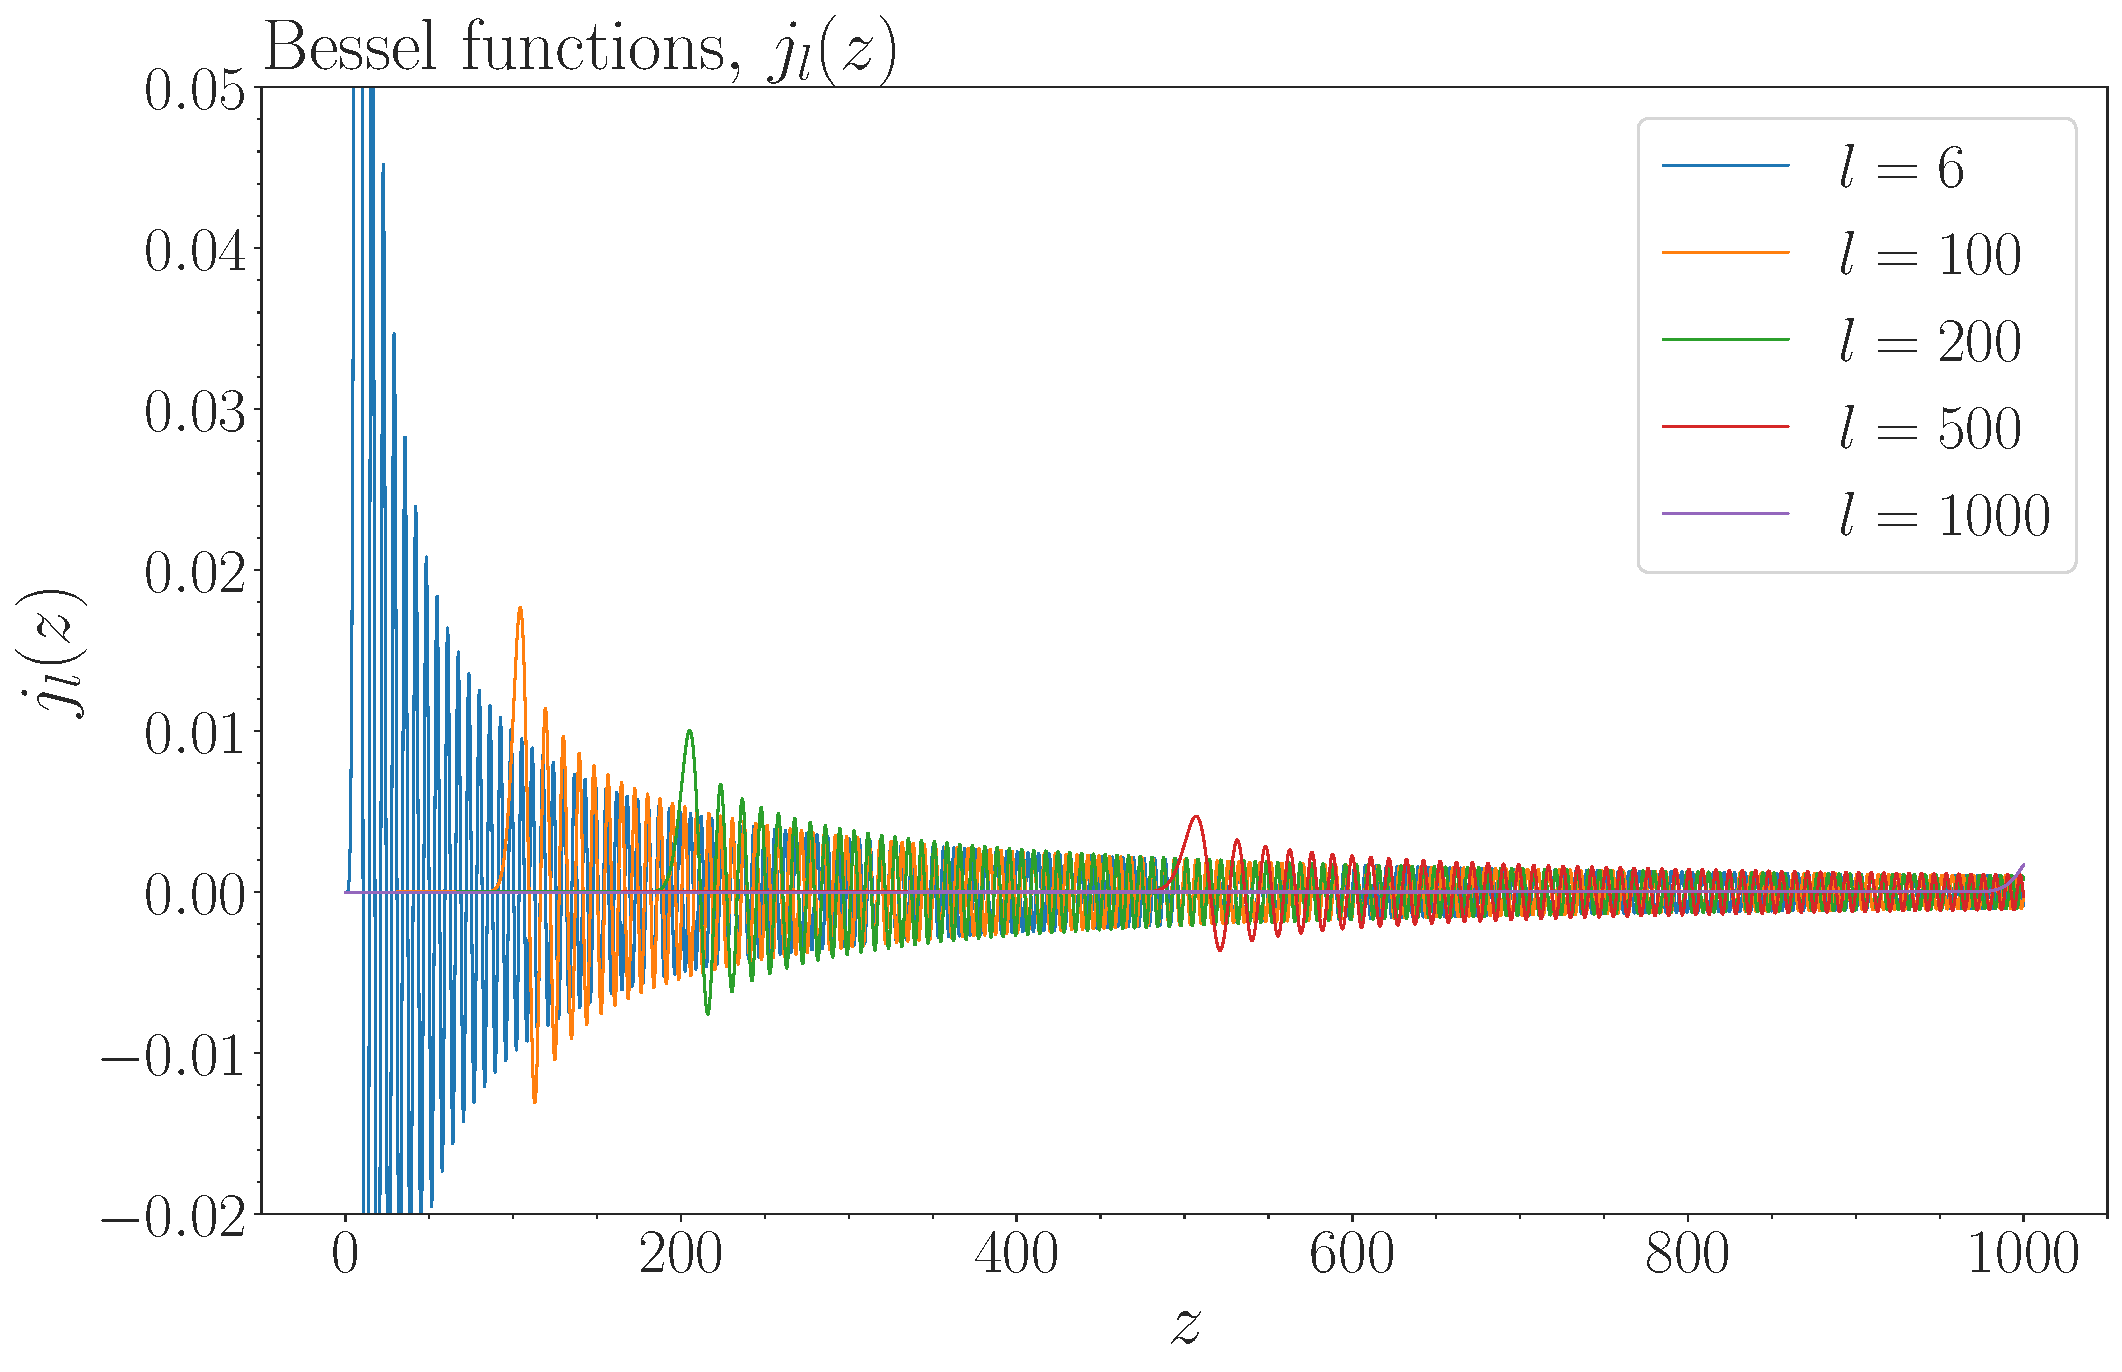
\includegraphics[width=\linewidth]{bessel.pdf}
            \caption{The spherical Bessel function for selected $l$-values.}
            \label{fig:m4:bessel}
        \end{figure}
        One ending note is that if the argument $z$ of the spherical Bessel functions are too large, some functions for finding it may break down, so proceed with caution. 

    \subsubsection{Line of sight integration}
        We are now ready to perform the actual line of sight integration from ~\cref{eq:m3:theory:line_of_sight_integral_definition}. We are supposed to integrate from $-\infty$ until today, but by investigating the integrand we may simplify this. ~\cref{fig:m4:LOS_integrand} show the integrand for a selected number of $l$-s. From the discussion of the source function in ~\cref{sec:m3:theory:line_of_sight}, we would expect most of its contribution to be around the time of recombination. This is emphasized in the plot, and we also see some effects at later times, up until today. These are the correction effects to the source function, which we need to take into account. The take home message is that there is very limited contribution from the time before recombination, so we choose some time right before recombination from which we start the integration. We must also here pay close attention to the sampling of the integrand because of the oscillations, and because it is a function of both $x$ and $k$. We sample w.r.t. $x$ as follows:
        \begin{equation}
            \Delta x = \frac{2\pi}{n_\mathrm{LOS}^{(x)}},
        \end{equation}
        and w.r.t. $k$ as:
        \begin{equation}
            \eta_0\Delta k = \frac{2\pi}{n_\mathrm{LOS}^{(k)}},
        \end{equation}
        where we use $n_\mathrm{LOS}^{(x)}=350$, and $n_\mathrm{LOS}^{(k)}=32$, since the integrand is a lot smoother in $k$ than $x$, we thus need a rather high resolution in $x$. 

        \begin{figure}
            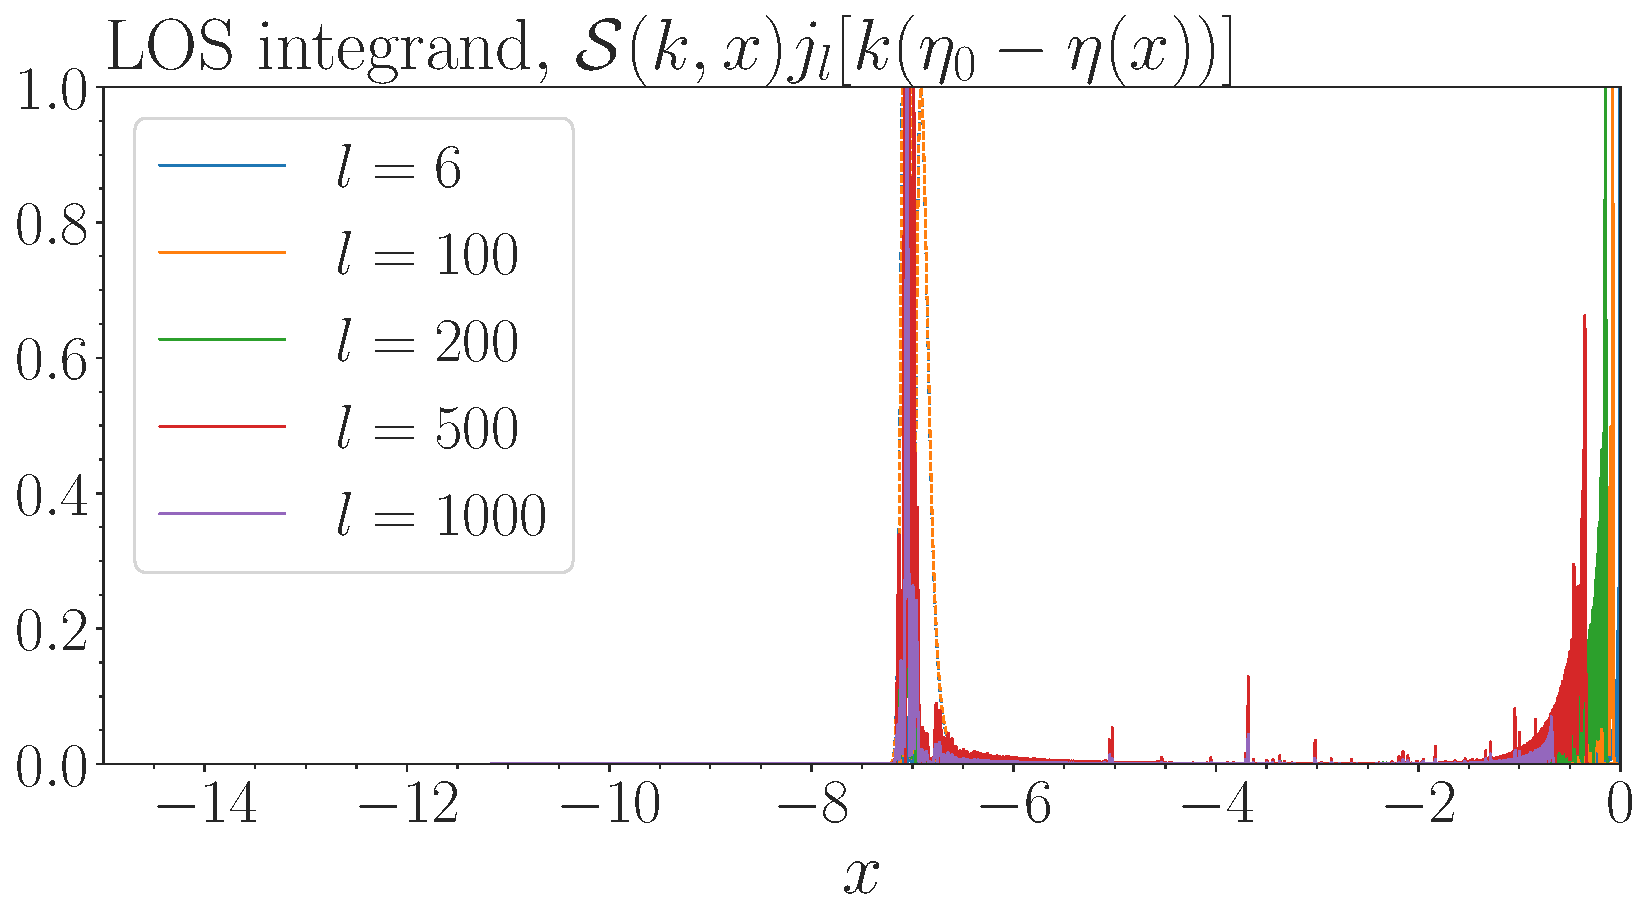
\includegraphics[width=\linewidth]{LOS_integrand.pdf}
            \caption{Integrand of LOS integral, mostly governed by the source function. The contribution is very limited before, but peaked during recombination. We have some contribution between recombination and today due to the corrections to the source function. The plot shows (but indistinguishable) values for $k=k_\mathrm{min}$ and $k=k_\mathrm{max}$ in order to highlight the extreme effects.}
            \label{fig:m4:LOS_integrand}
        \end{figure}

        The result of the line of sight integral is the transfer function $\T_l(k, \eta=\eta_0)$, and can be seen for the same selected values of $l$ in ~\cref{fig:m4:transfer_function}. It appears that our sampling was successful as we have captured the oscillations. This is by far the most time-consuming part of the integration, and the result is thus splined for easy access later on. 
        \begin{figure}
            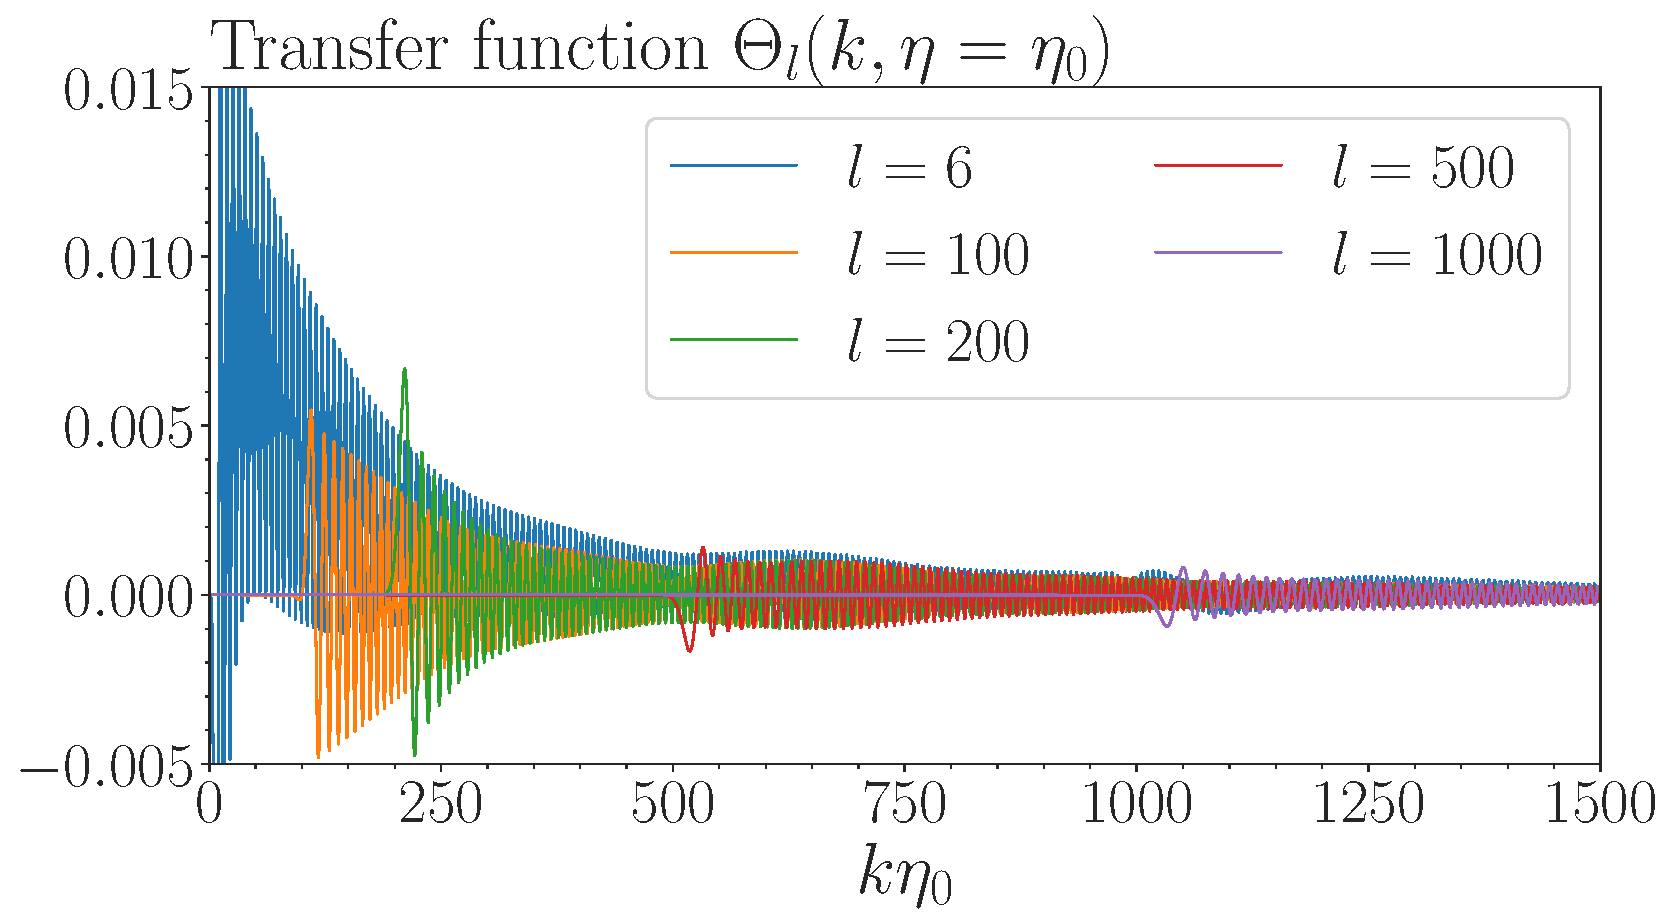
\includegraphics[width=\linewidth]{transfer_function.pdf}
            \caption{Transfer function after performing line of sight integration for a selected number of $l$-s, as function of $k$. }
            \label{fig:m4:transfer_function}
        \end{figure}
    \subsubsection{Integrate across $k$}
        When integating across $k$ in order to obtain the power spectrum $C_l$ the main dependence on $k$ is through the transfer function, so we use the same resolution as earlier for $k$. It is worth noting that integrating with respect to $\d k/k$ is equivalent to integrating with respect to $\d(\log{k})$, as long as we use the correct limits. It is thus straightforward to compute the angular power spectrum in ~\cref{eq:m4:theory:power_spectrum_logk}, and it is not very time-consuming since we have precomputed the transfer function already. ~\cref{fig:m4:C_l_integrand} shows the integrand of the angular power spectrum integral, which is just the transfer function weighted by $k$ (the primordial power spectrum is not included). 
        \begin{figure}
            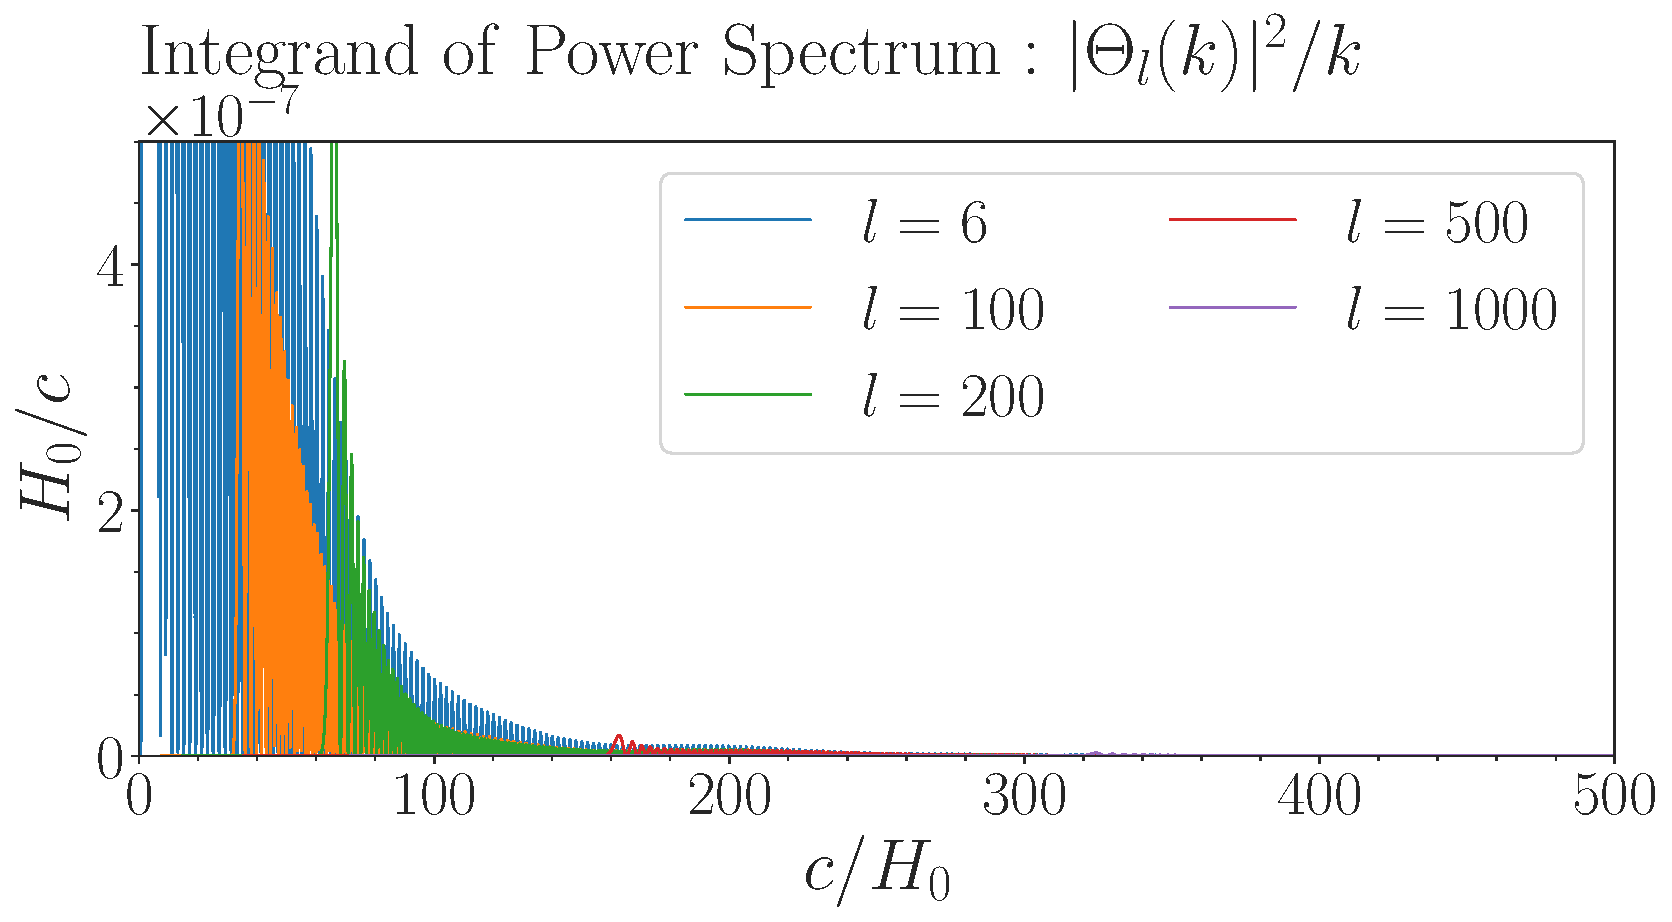
\includegraphics[width=\linewidth]{C_l_integrand.pdf}
            \caption{Integrand of the power spectrum integral as function of $k$, given for a selected number of $l$-s.}
            \label{fig:m4:C_l_integrand}
        \end{figure}


    \subsubsection{Numerical integration}
        Due to the large sampling rate when the functions are not smooth, there is no point in wasting computational resources on a more accurate numerical integrator than the \textit{trapezoidal method}. Since we specify samplings as constant spacing, we end up with a uniformly spaced domain, where we have $N$ discretised spaces and $N\Delta x= b-a$ where $b$ is the maximum value of the domain and $a$ the minimum. We approximate the finite integral as follows:
        \begin{equation}
            \int_a^bf(x)\d x \approx \left[ \sum_{i=1}^{N-1}f(x_i) + \frac{f(x_a)+f(x_b)}{2} \right]\Delta x.
        \end{equation}
        This method is used both when integrating across $x$ and $k$. 



\subsection{Results}\label{sec:m4:results}
    ~\cref{fig:m4:angular_power_spectrum} shows the angular power spectrum as function of photon multipole $l$. The blue drawn line is the main power spectrum, while the dotted lines are the four constituents of the power spectrum that arise from the source function in ~\cref{eq:m3:theory:source_function}. The red lines are observations taken from ~\cite{Planck2020}, and the turquoise shade shows the theoretical cosmic variance as given in ~\cref{eq:m4:theory:cosmic_variance}. As expected, since we ignore both polarisation and neutrinos there is a discrepancy between the observed values and the theoretical prediction. This is most prominent for larger $l$-s where the observational constraints are low due to high statistical accuracy. In discussing this results, we will focus on the three main parts of the plots, namely the \textit{Sachs-Wolfe plateau} for low $l$-s, the \textit{acoustic oscillations} for intermediate $l$-s and the \textit{diffusion damping} for high $l$-s. Lastly we discuss the matter power spectrum in, where we have obtained the observational data from ~\cite{Chabanier_2019} and ~\cite{Hlozek_2012}.
    \begin{figure}
        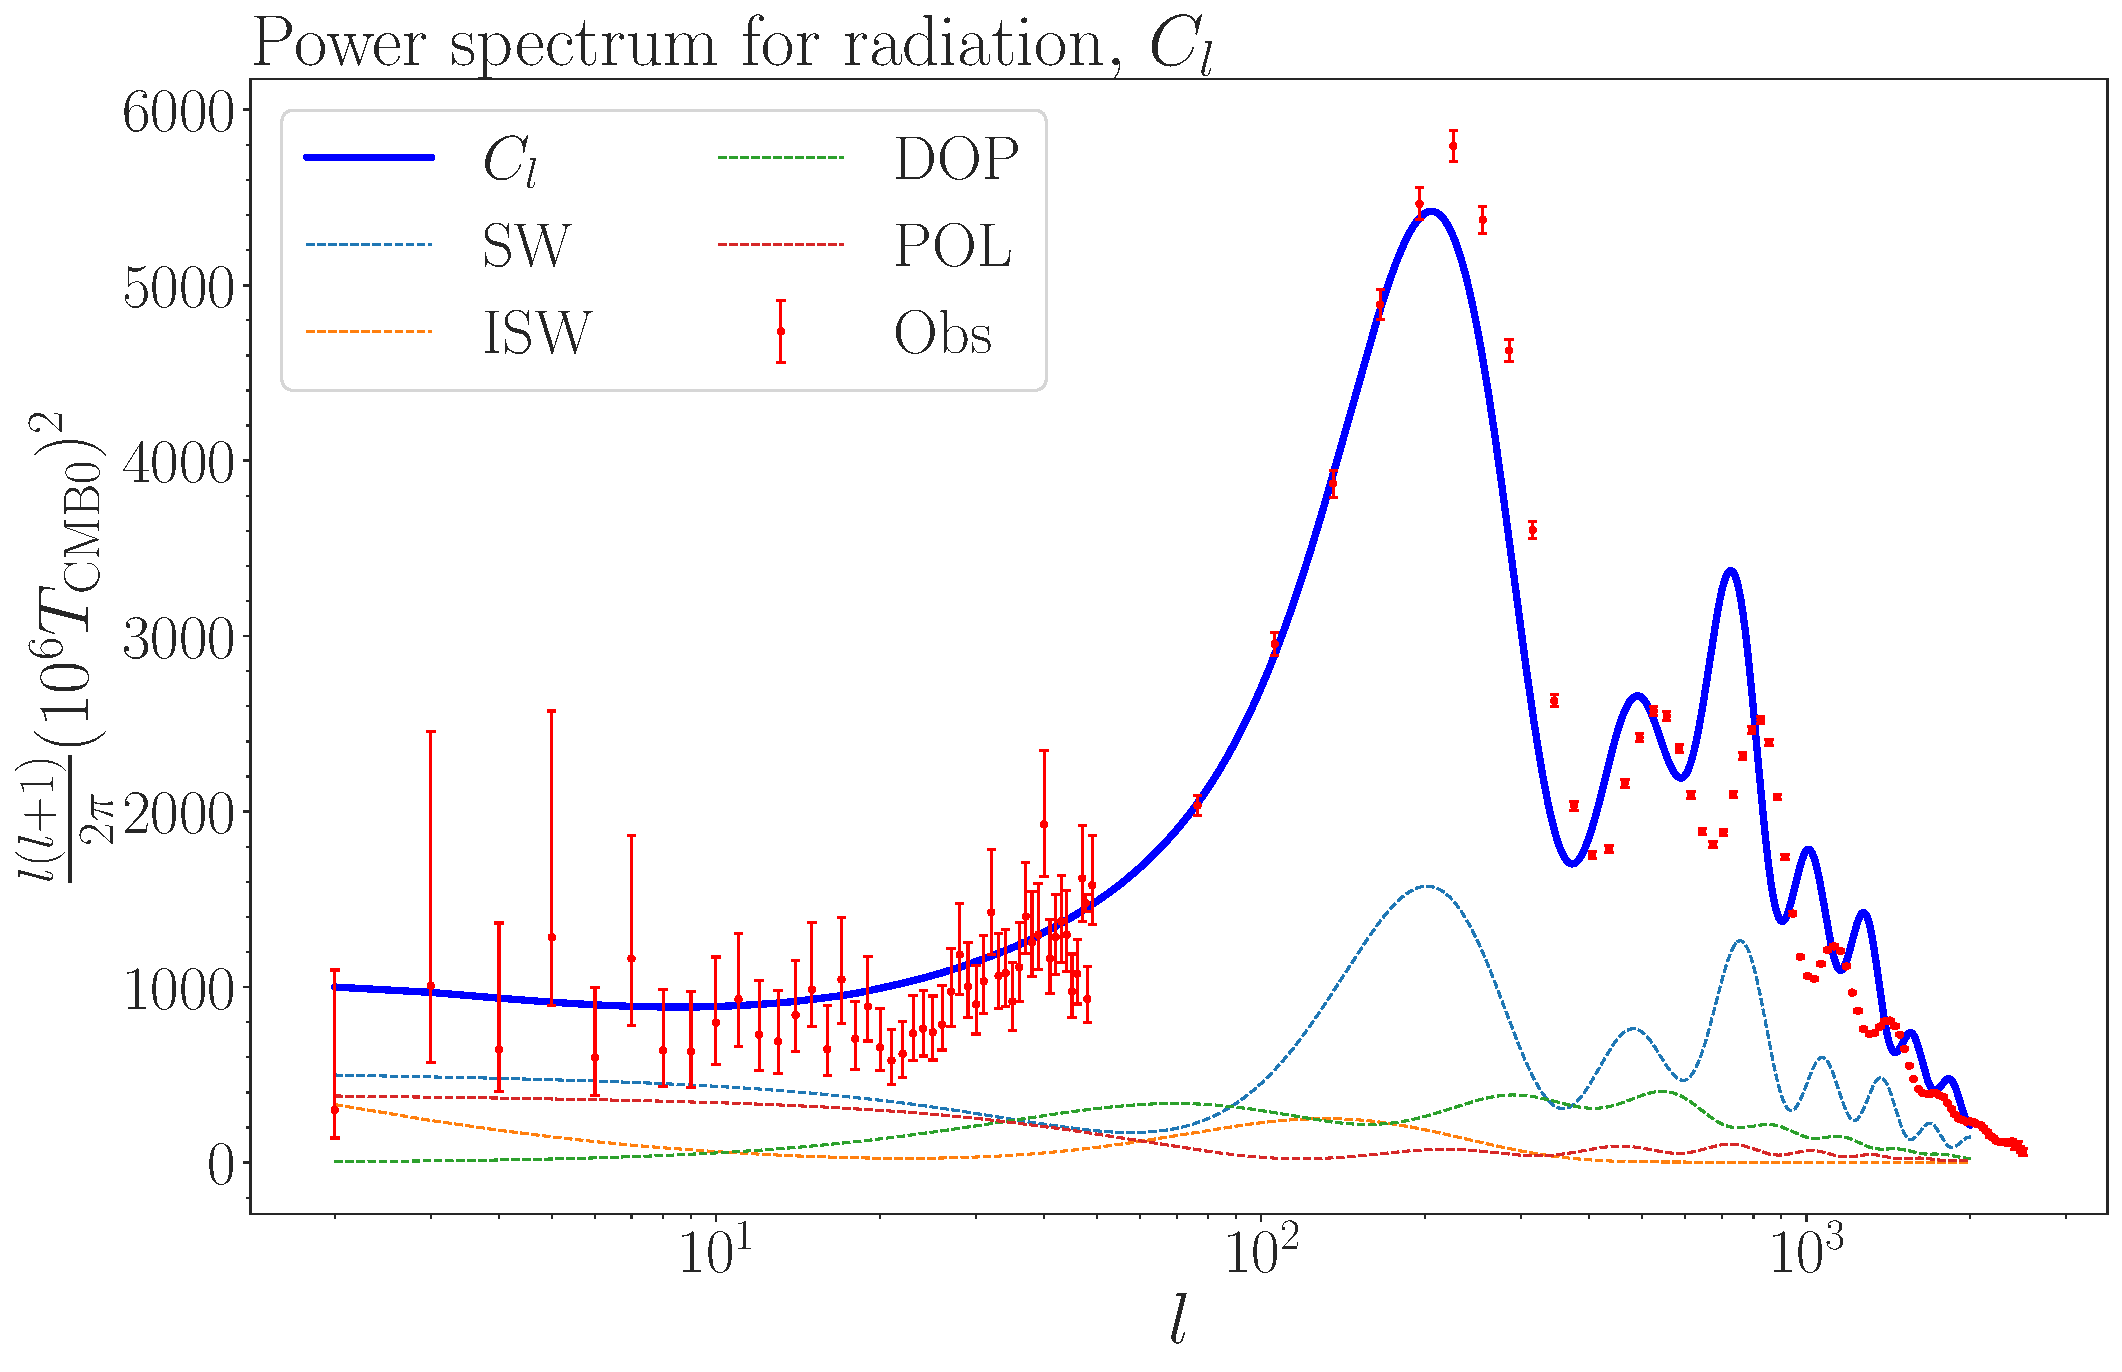
\includegraphics[width=\linewidth]{power_spectrum.pdf}
        \caption{Angular power spectrum as function of photon multipole $l$. The blue line shows the angular power spectrum itself with the intrinsic cosmic variance overplotted in turquoise. The dotted lines are the individual effect of the different constituents of the source function. The red error bars are observational constraints.}
        \label{fig:m4:angular_power_spectrum}
    \end{figure}
    \subsubsection{The Sachs-Wolfe plateau}
        The Sachs-Wolfe plateau is the part of the angular power spectrum that appear fairly flat for low $l$, i.e. large scales, hence it names. These large scale represent modes that had not yet entered the horison at the time of recombination. According to the Sachs-Wolfe term in the source function in ~\cref{eq:m3:theory:source_function}, the major contribution to the power spectrum are the temperature anisotropies present at the last scattering surface. This is the main contributor to the transfer function and thus the power spectrum itself. These effects are described by the photon monopole, and the value of the gravitational perturbation, $\Psi$, whose main effect slowed the photons down through gravitational redshift.\footnote{Plus a small quadrupole correction.} For large scales, that have not yet entered the horison at the time of last scattering, the fluctuation to the gravitational perturbation have not yet been affected by causal physics. As a result, they closely resemble the initial perturbations induced by inflation. 

        Thus, the Sachs-Wolfe plateau may be understood as a tracer of the primordial power spectrum. If we continue to assume this take the form of a Harrison-Zel'dovich spectrum parametrised by the amplitdue $A_s$ and spectral index $n_s$ we are able to estimate the former by considering the amplitude of the Sachs-Wolfe plateau, and the latter by its shape. $n_s=1$ would generate a flat primordial power spectrum, whereas $n_s>1$ would give emphasis to small scales and vice versa. 

    \subsubsection{Acoustic oscillations}

    \subsubsection{The damping tail}


    \subsubsection{The matter power spectrum}
    
    \begin{figure}
        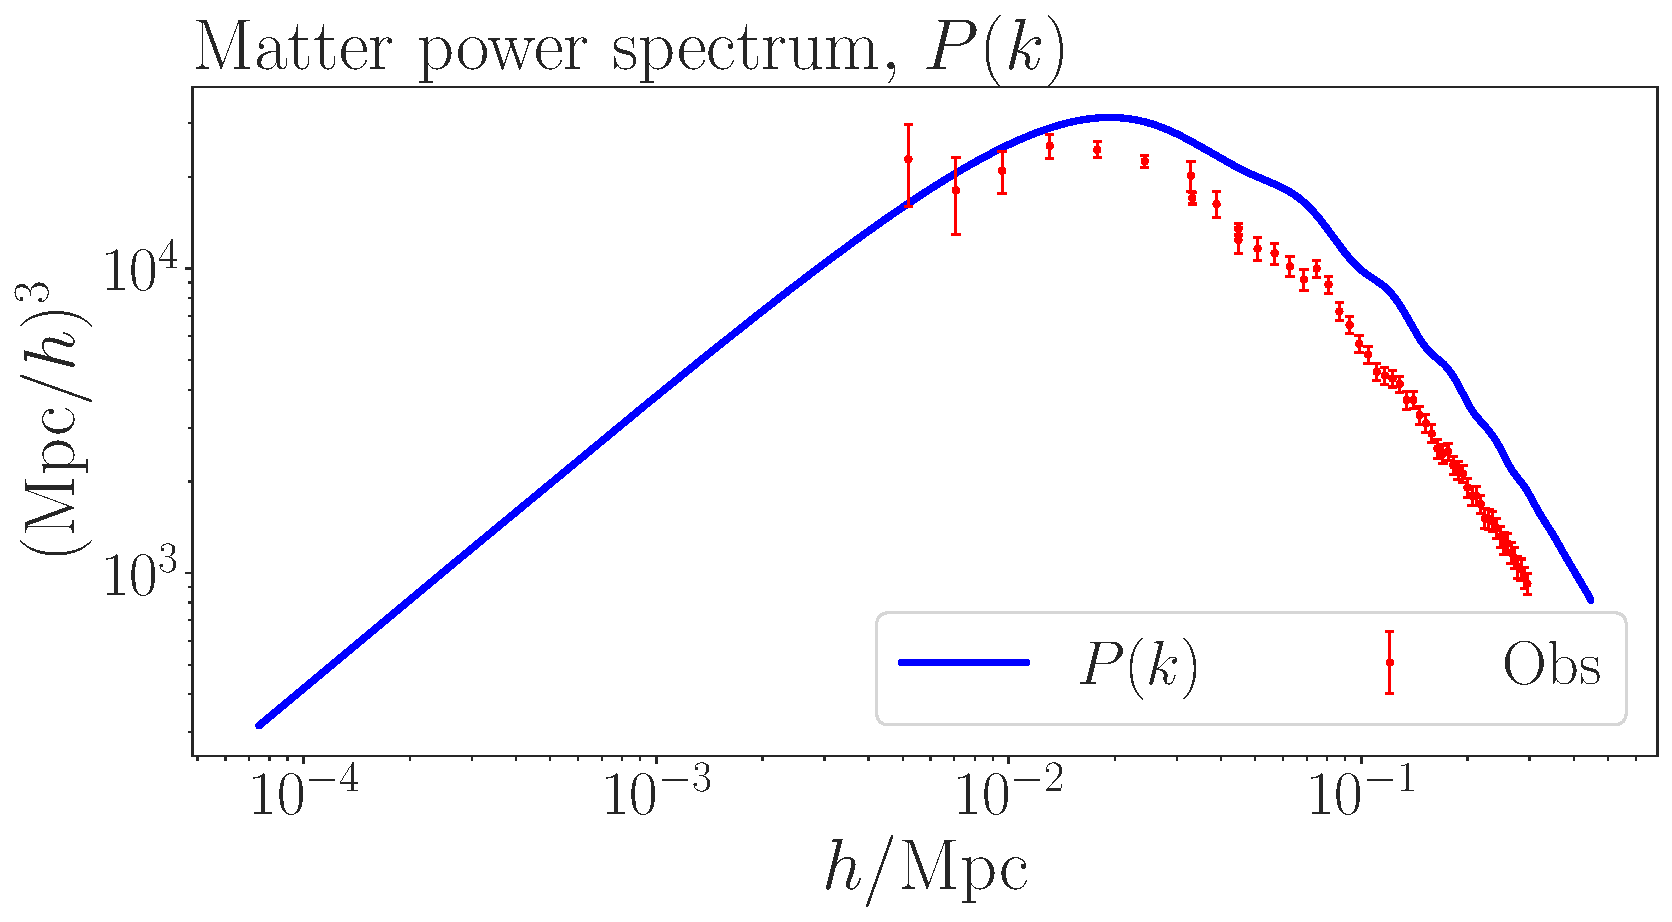
\includegraphics[width=\linewidth]{matter_power_spectrum.pdf}
        \caption{Matter power spectrum as function of wavenumber $k$. The violet dotted line the equality scale, which is the wavenumber that correspond to the mode entering the horison at the time of radiation-matter equality. The red error bars are observational constraints.}
        \label{fig:m4:matter_power_spectrum}
    \end{figure}

\newpage
\section{Conclusion}\label{sec:conclusion}

Throughout this project we have investigated the unperturbed FLRW background and its properties, the epoch of recombination, and perturbation to the FLRW background. All of this enabled us to construct the angular power spectrum of the CMB and the matter power spectrum for the total density contrast; quantities which we were able to compare with actual physical observables. These predictions were quite accurate for large scales, but showing a discrepancy larger than the observational uncertainties for the small scales. This is because we ignore the effect of neutrinos, polarisation and heavier elements when evolving the perturbation equations. We also do not consider the epoch of reionisation. Including all these effect would be a natural next step in improving our model. However, we are able to qualitatively discuss the physics behind most aspects of both power spectrums, having succeeded in our initial aim of producing a pipeline that numerically calculated the CMB power spectrum and matter power spectrum, given some cosmological model.


%======================================================
%
%   End of document
%
%======================================================

\bibliography{references/ref}

% \appendix

% \section{Derivation of the Friedmann equations}\label{app:friedmann}
%     The Einstein equation relates the curvature of spacetime to the distribution of matter and energy within it, and is given by:

%     $$G_{\mu\nu} = 8\pi T_{\mu\nu}$$

%     where $G_{\mu\nu}$ is the Einstein tensor, which describes the curvature of spacetime, and $T_{\mu\nu}$ is the stress-energy tensor, which describes the distribution of matter and energy. To derive the Friedmann equations from this equation, we need to first make some assumptions about the geometry and matter content of the universe.

%     We assume that the universe is homogeneous and isotropic, which implies that the metric for the universe can be written in the following form:

%     $$ds^2 = -c^2 dt^2 + a(t)^2\left[\frac{dr^2}{1-kr^2} + r^2(d\theta^2 + \sin^2\theta d\phi^2)\right]$$

%     where $a(t)$ is the scale factor of the universe, $k$ is the curvature of space, and $c$ is the speed of light.

%     With this metric, we can compute the Christoffel symbols, which describe the connection coefficients of spacetime, using the following equation:

%     $$\Gamma^{\rho}{\mu\nu} = \frac{1}{2}g^{\rho\sigma}\left(\frac{\partial g{\sigma\mu}}{\partial x^{\nu}}+\frac{\partial g_{\sigma\nu}}{\partial x^{\mu}}-\frac{\partial g_{\mu\nu}}{\partial x^{\sigma}}\right)$$

%     where $g_{\mu\nu}$ is the metric tensor and $g^{\mu\nu}$ is its inverse. After computing all the non-zero Christoffel symbols, we can use them to calculate the components of the Einstein tensor, which are given by:

%     $$G_{00} = -3\frac{\ddot{a}}{a} - 3\frac{k}{a^2}$$
%     $$G_{ij} = (\ddot{a} + 2\frac{\dot{a}^2}{a^2} + 2\frac{k}{a^2})\delta_{ij}$$

%     where $\delta_{ij}$ is the Kronecker delta.

%     Next, we need to specify the stress-energy tensor, which describes the distribution of matter and energy in the universe. For a homogeneous and isotropic universe, this tensor takes the form of a perfect fluid, with energy density $\rho$ and pressure $p$ given by:

%     $$T_{00} = \rho c^2$$
%     $$T_{ij} = p a^2\delta_{ij}$$

%     Substituting these expressions for the stress-energy tensor into the Einstein equation, and equating the components of the Einstein tensor to the corresponding components of the stress-energy tensor, we obtain the following equations:

%     $$\frac{\ddot{a}}{a} = -\frac{4\pi G}{3}(\rho + 3p) + \frac{\Lambda}{3}$$
%     $$(\frac{\dot{a}}{a})^2 + \frac{k}{a^2} = \frac{8\pi G}{3}\rho + \frac{\Lambda}{3}$$

%     These are the Friedmann equations, which describe the evolution of the scale factor and energy density of the universe. The first equation describes the acceleration of the expansion of the universe, and the second equation relates the expansion rate to the energy density and curvature of space.


%     In order to compute the Christoffel symbols, we start with the metric for the universe, which we assume is homogeneous and isotropic:

%     $$ds^2 = -c^2 dt^2 + a(t)^2\left[\frac{dr^2}{1-kr^2} + r^2(d\theta^2 + \sin^2\theta d\phi^2)\right]$$

%     where $a(t)$ is the scale factor of the universe, $k$ is the curvature of space, and $c$ is the speed of light.

%     The non-zero components of the metric tensor are:

%     $$g_{00} = -c^2, \quad g_{11} = a^2\frac{1}{1-kr^2}, \quad g_{22} = a^2r^2, \quad g_{33} = a^2r^2\sin^2\theta$$

%     Using the metric tensor, we can calculate the inverse metric tensor:

%     $$g^{00} = -\frac{1}{c^2}, \quad g^{11} = \frac{1-kr^2}{a^2}, \quad g^{22} = \frac{1}{a^2r^2}, \quad g^{33} = \frac{1}{a^2r^2\sin^2\theta}$$

%     We can now use these expressions to compute the Christoffel symbols, which are given by:

%     $$\Gamma^0_{00} = \Gamma^0_{i0} = \Gamma^i_{00} = 0$$

%     $$\Gamma^i_{jk} = \frac{1}{2}g^{il}(\frac{\partial g_{jl}}{\partial x^k}+\frac{\partial g_{kl}}{\partial x^j}-\frac{\partial g_{jk}}{\partial x^l})$$

%     where $i,j,k,l$ are indices running over the three spatial coordinates, and $x^j$ are the coordinates themselves.

%     For the diagonal terms, we have:

%     $$\Gamma^1_{11} = -\frac{kr}{1-kr^2}, \quad \Gamma^2_{22} = -r(1-kr^2), \quad \Gamma^3_{33} = -r(1-kr^2)\sin^2\theta$$

%     For the off-diagonal terms, we have:

%     $$\Gamma^1_{22} = \Gamma^1_{33} = \frac{1}{r}, \quad \Gamma^2_{33} = -\sin\theta\cos\theta$$

%     All other Christoffel symbols are either zero or can be obtained by symmetry. We can now use these Christoffel symbols to calculate the components of the Einstein tensor, which are given by:

%     $$G_{00} = -3\frac{\ddot{a}}{a} - 3\frac{k}{a^2}$$
%     $$G_{ij} = (\ddot{a} + 2\frac{\dot{a}^2}{a^2} + 2\frac{k}{a^2})\delta_{ij}$$

%     where $\delta_{ij}$ is the Kronecker delta.

%     Next, we need to specify the stress-energy tensor, which describes the distribution of matter and energy in the universe. For a homogeneous and isotropic universe, this tensor takes the form of a perfect fluid, with energy density $\rho$ and pressure $p$ given by:

%     $$T_{00} = \rho c^2$$

%     $$T_{ij} = p a^2 \delta_{ij}$$

%     Plugging these expressions into the Einstein equation, $G_{\mu\nu} = \frac{8\pi G}{c^4}T_{\mu\nu}$, we get:

%     $$-3\frac{\ddot{a}}{a}-3\frac{k}{a^2}=\frac{8\pi G}{c^4}\rho c^2$$

%     $$(\ddot{a}+2\frac{\dot{a}^2}{a^2}+2\frac{k}{a^2})\delta_{ij}=-\frac{8\pi G}{c^4}p a^2 \delta_{ij}$$

%     Simplifying the second equation by dividing both sides by $\delta_{ij}$ and using the first equation to eliminate the term involving $k$, we get:

%     $$\ddot{a}+2\frac{\dot{a}^2}{a}-\frac{8\pi G}{3c^2}(\rho + \frac{3p}{c^2})=0$$

%     This is the first Friedmann equation, which describes the evolution of the scale factor of the universe. The second Friedmann equation can be obtained by taking the trace of the Einstein equation, which gives:

%     $$3\frac{\ddot{a}}{a}+3\frac{k}{a^2}=4\pi G(\rho+\frac{3p}{c^2})$$

%     Eliminating $k$ using the first Friedmann equation, we get:

%     $$\left(\frac{\dot{a}}{a}\right)^2=\frac{8\pi G}{3}\rho-\frac{kc^2}{a^2}$$

%     This is the second Friedmann equation, which relates the Hubble parameter (the time derivative of the scale factor) to the energy density of the universe.

%     Thus, we have derived the Friedmann equations from the Einstein equation by explicitly computing all the Christoffel symbols and using the stress-energy tensor of a perfect fluid.

\section{Useful derivations}\label{app:derivations}
    \subsection{Angular diameter distance}
        This is related to the physical distance of say, an object, whose extent is small compared to the distance at which we observe is. If the extension of the object is $\Delta s$, and we measure an angular size of $\Delta\theta$, then the angular distance to the object is:

        \begin{equation}\label{eq:app:derivations:angular_distance}
            d_A = \frac{\Delta s}{\Delta\theta} = \frac{\d s}{\d\theta} = \sqrt{e^{2x}r^2} = e^xr,
        \end{equation}
        where we inserted for the line element $\d s$ as given in equation \cref{eq:m1:theory:fundamentals:FLWR_line_element}, and used the fact that $\d t/\d \theta = \d r/\d\theta = \d\phi/\d\theta  = 0$ in polar coordinates. 

    \subsection{Luminosity distance}
        If the intrinsic luminosity, $L$ of an object is known, we can calculate the flux as: $F=L/(4\pi d_L^2)$, where $d_L$ is the luminosity distance. It is a measure of how much the light has dimmed when travelling from the source to the observer. For further analysis we observe that the luminosity of objects moving away from us is changing by a factor $a^{-4}$ due to the energy loss of electromagnetic radiation, and the observed flux is changed by a factor $1/(4\pi d_A^2)$. From this we draw the conclusion that the luminosity distance may be written as:
        \begin{equation}
            d_L = \sqrt{\frac{L}{4\pi F}} = \sqrt{\frac{d_A^2}{a^4}} = e^{-x}r 
        \end{equation}

    \subsection{Differential equations}
    From the definition of $e^x\d\eta = c\d t$ we have the following:
    \begin{equation}
        \begin{split}
            \dv{\eta}{t} &= \dv{\eta}{x}\dv{x}{t}= \dv{\eta}{x}H = e^{-x}c \\
            \implies \dv{\eta}{x} &= \frac{c}{\Hp}.
        \end{split}
    \end{equation}

    Likewise, for $t$ we have:
    \begin{equation}
        \begin{split}
            \dv{\eta}{t} &= \dv{\eta}{x}\dv{x}{t} = \dv{x}{t}\frac{c}{\Hp} = e^{-x}c\\
            \implies \dv{t}{x} &= \frac{e^x}{\Hp} = \frac{1}{H}.
        \end{split}
    \end{equation}


\section{Sanity checks}\label{app:sanity}
\subsection{For $\Hp$}
    We start with the Hubble equation from \cref{eq:m1:lambdaCDM:conformal_Hubble_equation} and realize that we may write any derivative of $U$ as
    \begin{equation}
        \dv[n]{U}{x} = \sum_i(-\alpha_i)^n\O_{i0}\expe{-\alpha_ix}.
    \end{equation}

    We further have:
    \begin{equation}
        \dv{\Hp}{x} = \frac{H_0}{2}U^{-\frac{1}{2}}\dv{U}{x},
    \end{equation}

    and
    
    \begin{equation}
        \begin{split}
            \dv[2]{\Hp}{x} &= \dv{}{x}\dv{\Hp}{x}\\
            &= \frac{H_0}{2}\left[\dv{U}{x}\left(\dv{}{x}U^{-\frac{1}{2}}\right) + U^{-\frac{1}{2}}\left(\dv{}{x}\dv{U}{x}\right)\right]\\
            &=H_0\left[\frac{1}{2U^{\frac{1}{2}}}\dv[2]{U}{x} - \frac{1}{4U^{\frac{3}{2}}}\left(\dv{U}{x}\right)^2\right]
        \end{split}
    \end{equation}


    Multiplying both equations with $\Hp^{-1} = 1/(H_0U^{\frac{1}{2}})$ yield the following:

    \begin{equation}
        \frac{1}{\Hp}\dv{\Hp}{x} = \frac{1}{2U}\dv{U}{x},
    \end{equation}

    and 

    \begin{equation}
        \begin{split}
            \frac{1}{\Hp}\dv[2]{\Hp}{x} &= \frac{1}{2U}\dv[2]{U}{x} - \frac{1}{4U^2}\left(\dv{U}{x}\right)^2 \\
            &= \frac{1}{2U}\dv[2]{U}{x}-\left(\frac{1}{\Hp}\dv{U}{x}\right)^2
        \end{split}
    \end{equation}

    We now make the assumption that one of the density parameters dominate $\O_i>> \sum_{j\neq i}\O_i$, enabling the following approximation:
    
    \begin{equation}
        \begin{split}
            U &\approx \O_{i0}\expe{-\alpha_ix} \\
            \dv[n]{U}{x} &\approx (-\alpha_i)^n\O_{i0}\expe{-\alpha_ix},
        \end{split}
    \end{equation}
    from which we are able to construct:
    \begin{equation}
        \frac{1}{\Hp}\dv{\Hp}{x} \approx \frac{-\alpha_i\O_{i0}\expe{-\alpha_ix}}{2\O_{i0}\expe{-\alpha_ix}} = -\frac{\alpha_i}{2},
    \end{equation}
    and
    \begin{equation}
        \begin{split}
            \frac{1}{\Hp}\dv[2]{\Hp}{x} &\approx \frac{\alpha^2\O_{i0}\expe{-\alpha_ix}}{2\O_{i0}\expe{-\alpha_ix}} - \left(\frac{\alpha_i}{2}\right)^2 \\
            &= \frac{\alpha_i^2}{2} - \frac{\alpha_i^2}{4} = \frac{\alpha_i^2}{4}
        \end{split}
    \end{equation}
    which are quantities which should be constant in different regimes and we can easily check if our implementation of $\Hp$ is correct, which is exactly what we sought. 

\subsection{For $\eta$}

    In order to test $\eta$ we consider the definition, solve the integral and consider the same regimes as above, where one density parameter dominates:

    \begin{equation}
        \begin{split}
            \eta &= \int_{-\infty}^x \frac{c\d x}{\Hp} = \frac{-2c}{\alpha_i}\int_{x=-\infty}^{x=x}\frac{\d\Hp}{\Hp^2} \\
            &= \frac{2c}{\alpha_i}\left(\frac{1}{\Hp(x)}-\frac{1}{\Hp(-\infty)}\right),
        \end{split}
    \end{equation}
    where we have used that:
    \begin{equation}
        \begin{split}
            \dv{\Hp}{x} &= -\frac{\alpha_i}{2}\Hp \\
            \implies \d x &= -\frac{2}{\alpha_i\Hp}\d\Hp.
        \end{split}
    \end{equation}
    
    Since we consider regimes where one density parameter dominates, we have that $\Hp(x)\propto \sqrt{\expe{-\alpha_ix}}$, meaning that we have:
    \begin{equation}
        \left(\frac{1}{\Hp(x)}-\frac{1}{\Hp(-\infty)}\right) \approx 
        \begin{cases}
            \frac{1}{\Hp} \quad &\alpha_i>0 \\
            -\infty \quad &\alpha_i <0.
        \end{cases}
    \end{equation}
    Combining the above yields:
    \begin{equation}
        \frac{\eta\Hp}{c} \approx 
        \begin{cases}
            \frac{2}{\alpha_i} \quad &\alpha_i>0 \\
            \infty \quad &\alpha_i<0.
        \end{cases}
    \end{equation}
    Notice the positive sign before $\infty$. This is due to $\alpha_i$ now being negative. 
    


\end{document}